\documentclass[11pt,a4paper, DIV=12]{report}
\usepackage[utf8]{inputenc}
\usepackage[english]{babel}
\usepackage[T1]{fontenc}
\usepackage[numbers,square]{natbib}
\usepackage[a4paper, margin=1.2in]{geometry}
\usepackage{pdfpages}
%\usepackage{showframe}
\usepackage{booktabs}
\usepackage{xcolor}
\usepackage{graphicx}
\usepackage{tikz}
\usetikzlibrary{shapes,snakes,patterns, positioning}
\usepackage{caption}
\usepackage{subcaption}
\usepackage{afterpage}
\usepackage{tablefootnote}
%\KOMAoption{DIV}{12} %instead of ,left=2cm,right=2cm,top=2cm,bottom=2.2cm etc
%\addtokomafont{disposition}{\rmfamily} % serifes in headings

\pagestyle{plain}
%\addtokomafont{section}{\clearpage}

%\addtolength{\footskip}{-1.5cm}

%%Mathe - Imports
\usepackage{amsmath}
\usepackage{amsfonts}
\usepackage{amssymb}
\usepackage{mathrsfs}
\usepackage{mathtools}
\usepackage{amsthm}
\usepackage[theorems,many]{tcolorbox}
\tcbuselibrary{breakable}
\allowdisplaybreaks
\usepackage[lightning]{stmaryrd}
\usepackage{extarrows}

\usepackage{lmodern}
\usepackage[hidelinks]{hyperref}
\usepackage{float}
\usepackage{enumitem}

\setlength{\parindent}{0pt}

\newcommand{\uri}[1]{\texttt{#1}}

\usepackage[nodayofweek]{datetime}

%% Mathe - Formatierungszeugs
\theoremstyle{definition}
\newtcbtheorem[]{BspI}{Example}{%
	before skip = 11pt,
	colback=blue!5,
	colframe=blue!35!black,
	fonttitle=\bfseries,
	breakable,
	enhanced jigsaw,
	lines before break=3
	}{Bsp}

\definecolor{block-gray}{gray}{0.95}

\newtcbtheorem[]{DefI}{Definition}{%
    colback=white,
    colframe=white,
    %grow to right by=-10mm,
    %grow to left by=-10mm, 
    boxrule=0pt,
    boxsep=0pt,
    breakable,
    enhanced jigsaw,
    borderline west={3pt}{0pt}{black},
    %colbacktitle={block-gray},
    coltitle={black},
    fonttitle={\bfseries},
    attach title to upper={\\},
    lines before break=3
    }{Def}

\newtcbtheorem[]{SatzI}{Lemma}{%
    colback=white,
    colframe=white,
    %grow to right by=-10mm,
    %grow to left by=-10mm, 
    boxrule=0pt,
    boxsep=0pt,
    breakable,
    enhanced jigsaw,
    borderline west={3pt}{0pt}{red},
    %colbacktitle={block-gray},
    coltitle={black},
    fonttitle={\bfseries},
    attach title to upper={\\},
    lines before break=3
    }{S}
    
\newenvironment{Bsp}[2]{\vspace{0.2cm}\begin{BspI}{#1}{#2}}{\end{BspI}\vspace{0.2cm}}
\newenvironment{Satz}[2]{\vspace{0.2cm}\begin{SatzI}{#1}{#2}}{\end{SatzI}\vspace{0.2cm}}
\newenvironment{Def}[2]{\vspace{0.2cm}\begin{DefI}{#1}{#2}}{\end{DefI}\vspace{0.2cm}}


\setlist[description]{font=\normalfont\itshape\space}

\usepackage{listings}
\usepackage[scaled=0.7]{beramono}


\renewcommand\thesection{\arabic{chapter}.\arabic{section}}
\renewcommand\thesubsection{\arabic{chapter}.\arabic{section}.\arabic{subsection}}
\renewcommand\thesubsubsection{\arabic{chapter}.\arabic{section}.\arabic{subsection}.\arabic{subsubsection}}

% Outer Join Symbols
\def\ojoin{\setbox0=\hbox{$\bowtie$}%
  \rule[-.02ex]{.25em}{.4pt}\llap{\rule[\ht0]{.25em}{.4pt}}}
\def\leftouterjoin{\mathbin{\ojoin\mkern-5.8mu\bowtie}}
\def\rightouterjoin{\mathbin{\bowtie\mkern-5.8mu\ojoin}}
\def\fullouterjoin{\mathbin{\ojoin\mkern-5.8mu\bowtie\mkern-5.8mu\ojoin}}
\newenvironment{select}[1]{\sigma_{#1} \left(}{\right)}
\newenvironment{project}[1]{\pi_{#1} \left(}{\right)}
\newenvironment{aggregate}[2]{\Gamma_{#1~\#~#2} \left(}{\right)}
\newcommand{\rel}[1]{\MakeUppercase{\text{#1}}}
\newcommand{\join}[1]{\underset{\substack{#1}}{\bowtie}}
\newcommand{\semijoin}[1]{\underset{\substack{#1}}{\ltimes}}
\newcommand{\naturaljoin}{\bowtie}
\newcommand{\antisemijoin}[1]{\underset{\substack{#1}}{~\overline{\ltimes}~}}


\sloppy

%% Pseudocode - Imports
\usepackage{algorithm}
\usepackage{algpseudocode}
\floatname{function}{algorithm}
\algnewcommand\algorithmicforeach{\textbf{for each}}
\algdef{S}[FOR]{ForEach}[1]{\algorithmicforeach\ #1\ \algorithmicdo}
\newenvironment{breakablealgorithm}
  {% \begin{breakablealgorithm}
   \begin{center}
     \refstepcounter{algorithm}% New algorithm
     \hrule height.8pt depth0pt \kern2pt% \@fs@pre for \@fs@ruled
     \renewcommand{\caption}[2][\relax]{% Make a new \caption
       {\raggedright\textbf{\fname@algorithm~\thealgorithm} ##2\par}%
       \ifx\relax##1\relax % #1 is \relax
         \addcontentsline{loa}{algorithm}{\protect\numberline{\thealgorithm}##2}%
       \else % #1 is not \relax
         \addcontentsline{loa}{algorithm}{\protect\numberline{\thealgorithm}##1}%
       \fi
       \kern2pt\hrule\kern2pt
     }
  }{% \end{breakablealgorithm}
     \kern2pt\hrule\relax% \@fs@post for \@fs@ruled
   \end{center}
  }

\begin{document}
\begin{titlepage}
%	\begin{figure}[ht]
%	\flushright
%	\includegraphics[width=0.08\textwidth]{../DATA/FHAachen-logo2010.png}\par		%Logo oben rechts
%	\vspace{1cm}
%	\end{figure}
	
	\centering
	{\scshape\LARGE Gottfried Wilhelm Leibniz Universität Hannover\\Fakultät für Elektrotechnik und Informatik\par}   %Fach
	\vspace{1cm}
	{\scshape\Large Masterthesis\par}
	\vspace{1.5cm}
	{\huge\bfseries Supporting Explainable AI on Semantic Constraint Validation\par} 
	\vspace{2cm}
	{\Large Julian Alexander Gercke\par}
	\vfill
	
% Bottom of the page
	\begin{large}
	\begin{tabular}{l l}
		Matriculation number: & 10003079\\
		First evaluator: & Maria-Esther Vidal\\
		Seconde evaluator: & Sören Auer\\
		Supervisors: & Philipp D. Rohde and Maria-Esther Vidal\\
		Submission date: & \today
	\end{tabular}
	\end{large}
\end{titlepage}
\cleardoublepage

\thispagestyle{empty} 
\leavevmode%
\vspace*{\fill}\noindent
\begin{center}
  \textbf{DECLARATION OF AUTHORSHIP}
\end{center}

I, Julian Alexander Gercke, declare that this thesis titled, `Supporting Explainable AI on Semantic Constraint Validation' and the work presented in it are my own. I confirm that:

\begin{itemize} 
\item[\tiny{$\blacksquare$}] This work was done wholly or mainly while in candidature for a research degree at this University.
 
\item[\tiny{$\blacksquare$}] Where any part of this thesis has previously been submitted for a degree or any other qualification at this University or any other institution, this has been clearly stated.
 
\item[\tiny{$\blacksquare$}] Where I have consulted the published work of others, this is always clearly attributed.
 
\item[\tiny{$\blacksquare$}] Where I have quoted from the work of others, the source is always given. With the exception of such quotations, this thesis is entirely my own work.
 
\item[\tiny{$\blacksquare$}] I have acknowledged all main sources of help.
 
\item[\tiny{$\blacksquare$}] Where the thesis is based on work done by myself jointly with others, I have made clear exactly what was done by others and what I have contributed myself.
\\
\end{itemize}
\vspace{1cm}
\newlength\us
\settowidth{\us}{-~~~~~~Julian Alexander Gercke~~~~~~-}
\begin{minipage}{0.5\linewidth}
    \centering
    \begin{tabular}{p{\us}}\hline
    \centering\footnotesize Place, Date
    \end{tabular}
\end{minipage}
\begin{minipage}{0.5\linewidth}
    \centering
    \begin{tabular}{p{\us}}\hline
    \centering\footnotesize Julian Alexander Gercke
    \end{tabular}
\end{minipage}


\hfill\strut
\vspace*{\fill}

\clearpage 

%% ----------------------------------------------------------------
\begin{abstract}
There is a rising number of knowledge graphs available published through various sources. The enormous amount of linked data strives to give entities a semantic context. Using SHACL, the entities can be validated with respect to their context.
On the other hand, an increasing usage of AI models in productive systems comes with a great responsibility in various areas. Predictive models like linear, logistic regression, and tree-based models, are still frequently used as they come with a simple structure, which allows for interpretability. However, explaining models includes verifying whether the model makes predictions based on human constraints or scientific facts. This work proposes to use the semantic context of the entities in knowledge graphs to validate predictive models with respect to user-defined constraints; therefore, providing a theoretical framework for a model-agnostic validation engine based on SHACL. In a second step, the model validation results are summarized in the case of a decision tree and visualized model-coherently. Finally, the performance of the framework is evaluated based on a Python implementation.
\end{abstract}

\tableofcontents

\newpage

\chapter{Introduction}
    \label{section_introduction}
    AI is called explainable when a user of an AI model can understand the predictions a model makes. The user is enabled to not only interpret the model but trust the model through given reasoning of why a decision has been made. \cite{ibmExplainableAI, gilpin2018explaining} 

Knowledge graphs are used to store and connect data, promoting the cooperation between machines and humans. Therefore the data and its entities are stored in a way understandable for both. \cite{berners2002new}

Data is extracted from knowledge graphs for statistical analysis \cite{moghaddam2021literal2feature,cheng2011automated,narasimha2011liddm}. However, the process only uses the context of the extracted entities during the data mining process. On the other hand, embeddings represent the entity through its properties and links to other entities (i.e., latent vectors). Therefore, they incorporate the semantic context for later usage (e.g., clustering by embedding-based similarity measures \cite{embedding_similarity_measure}) but lake for explainability.
Finally, there are rule-based systems. Mohamed et al. \cite{excut} mine rules for comprehensible cluster labels. Halliwell et al. \cite{Halliwell2021} generate ground truth explanations for the link prediction task based on handcrafted rules. Even handcrafted rules show to suffer from understandability in some cases \cite{Halliwell2021}. 

In the area of the semantic web, SHACL engines are known for their capability to validate knowledge graphs against a set of constraints (i.e., rules). Therefore rating entities based on their integrity and trustability. 

This work aims to exploit SHACL engines to support the explainability of predictions made by machine learning models. The approach is naturally based on handcrafted constraints (i.e., rules), which should facilitate the generation of understandable explanations. Based on the constraints the approach will additionally increase the interpretability of AI models by annotating the model with constraint validation results. The constraint validation results will be based on the semantic context provided by a knowledge graph. 
Standard interpretability methods (e.g., LIME \cite{ribeiro2016should}, or Partial Dependence Plots \cite{friedman2001greedy}) do not take into consideration the context of the entities used to train the model or make predictions. Therefore Using the semantic context of entities in the described way is novel and closes a hole in interpretability methods. 

Recently, machine-learning-based techniques have been used to accelerate COVID-19-related drug discovery during the pandemic \cite{zhang2021ai}. Drugs found through these kinds of techniques need to be validated carefully. On a large scale, this highlights the importance of explainable AI. Most likely, the lack of explainability of the AI model used for drug discovery leads to the need to validate the results by hand. However, given the expertise in validating drugs, there are for sure constraints involving the training data and the assigned targets. These could have been used for automatic validation and a step toward better explainable AI. 
    
    \section{Motivating Example}
        The motivating example is about the social problem of vaccine hesitancy. This is a related problem, which got pronounced during the COVID-19 crisis, when the trust in official sources and scientific studies became a decisive factor in connection with the willingness to vaccinate \cite{petravic2021factors}. To counteract this behavior, one might imagine a predictive model based on a knowledge graph, which gives explainable recommendations to people, whether they should get vaccinated or not. Therefore, a social-themed knowledge graph about people and their COVID-19 vaccination status would be required. Due to privacy reasons, such a knowledge graph is not publicly available. However, one might expect that the introduction of electronic health records in more and more countries \cite{essen2018patient} will lead to broader availability of this kind of data to specific persons in the future. 
    
% The dataset
For the sake of comprehensibility, a tiny dataset (see figure \ref{fig:motivating_dataset}) is used for demonstration purposes. The dataset is not meant to be true in reality, but will help explain the approach (see chapter \ref{section_approach}). Each row in the table represents a type of sample, which has a weight assigned. This weight gives the proportion of this type of sample in the dataset. As described above, the example assumes a knowledge graph, which was used to extract the data. A small part of the knowledge graph is depicted in Figure \ref{fig:motivating_example_kg}. 
    
    \begin{figure}
        \centering
        \begin{tabular}{c|lclclc}
            \toprule
            weight & person & allergic\_to & gender & pregnant & country & vaccinated\\
            \midrule
            \midrule
            \(\frac{4}{12}\) & :Max & PEG & male & \(\bot\) & Germany & \(\bot\) \\
            \(\frac{1}{12}\) & :Maria & & female & \(\top\) & Germany & \(\bot\) \\
            \(\frac{6}{12}\) & :Eva   & & female & \(\bot\) & Germany & \(\top\) \\
            \(\frac{1}{12}\) & :Laura & PEG & female & \(\bot\) & Germany & \(\bot\) \\
            \bottomrule
        \end{tabular}
        \caption{Dataset about COVID-19 Vaccination}
        \label{fig:motivating_dataset}
    \end{figure}
    
    \begin{figure}
        \centering
        \includegraphics[width=\textwidth]{images/motivating_example/Dataset Covid-19 Part.png}
        \caption{Visualization of an RDF Graph containing some Instances of the Data}
        \label{fig:motivating_example_kg}
    \end{figure}
    
    % Knowledge Graph as Source of further insights (...this might even be the main reason, to perform constraint validation over data cleaning)   
    In this work, the goal is twofold. On the one hand, the work aims to use the additional context provided by a knowledge graph for a given set of entities. This is to be implemented to discover further insights into the patterns of machine learning models trained on the data extracted from the knowledge graph. On the other hand, a goal is to allow users to validate certain assumptions about the model using the context. To achieve that, user-defined constraints about the target of the machine learning model are validated against a knowledge graph and a model's predictions. When extracting a dataset, as in Figure \ref{fig:motivating_dataset}, from a knowledge graph, as in Figure \ref{fig:motivating_example_kg}, the graph structure of the data gets lost. In this example, there are the \uri{contact\_with} predicates, which get discarded. The example will show how this kind of semantic context, exclusively available in the knowledge graph, might be used to explain the model's predictions.
    
    % Data Quality Issues
    Available knowledge graphs suffer from data quality issues. For example, seven years ago, a paper identified certain substantial constraints over DBpedia \cite{mendes2012dbpedia}, which are frequently violated \cite{Kontokostas2014}. The situation has not changed until today \cite{valSPARQL}. This problem gets accelerated when learning from such kind of data. A model trying to generalize to this data will suffer from the same quality constraints as the data. Moreover, it will apply the recognized patterns to new data, which in turn, will also suffer from the same issues.
    
    Both, knowledge graphs as a source of further insights and data quality issues in knowledge graphs give rise to semantic constraint validation. This has the capability of identifying data points, which violate certain constraints and predictions made on the basis of these.% TODO: Somehow mention the concept of data constraints
    
    Let us assume a decision tree, trained on the given dataset, which recommends a person X, which is not allergic to PEG (included in COVID-19 vaccines) but is pregnant, not to get vaccinated (see Figure \ref{motivating_example_decision_tree}). 
    \begin{figure}
            \centering
            \includegraphics[width=0.6\textwidth]{images/visualizations/motivating_example_decision_tree_transparent.png}
            \caption{Decision tree trained on the dataset from figure \ref{fig:motivating_dataset} assuming $9999$ samples (n denotes the number of samples getting predictions assigned in the leaf) visualized using dtreeviz \cite{dtreeviz}}
            \label{motivating_example_decision_tree}
        \end{figure}
    \begin{figure}
            \centering
            \includegraphics[width=0.6\textwidth]{images/motivating_example/Annotated Decision Tree.png}
            \caption{The decision tree of figure \ref{motivating_example_decision_tree} annotated with the validation results of the example constraint. Pregnant persons not allergic to PEG are predicted not to be vaccinated, which violates the example constraint, given the semantic context of the persons in the knowledge graph.}
            \label{motivating_example_annotated_decision_tree}
    \end{figure}
   
   Although the decision tree is already inherently explainable, and it is, therefore, known why it recommends not getting vaccinated, it remains unclear whether the decision is rational with respect to human constraints or scientific facts. For example, there might be a constraint stating: \glqq{}\emph{Every pregnant person in Germany, which has more than 20 contacts with non-vaccinated persons should get vaccinated}\grqq{}. The decision tree alone cannot be used to validate the constraint. The underlying knowledge graph is needed to count the number of contacts with vaccinated persons. An option would be to include the number of contacts with non-vaccinated persons in the dataset, but that will not guarantee that the decision tree uses this data in a constraint conform way. 
    Further, one could exclude the examples from the dataset which violate the constraint. This might be a viable approach but will only eliminate the faulty examples from the dataset, which might, in turn, lead to a better-adapted model. However, edge cases not covered by the dataset and a generalized model might continue to give predictions violating the constraint. Therefore, it might be good to learn about the model trained on the available data.
    
    As a result, the approach implicitly validates the model given a set of constraints and the knowledge graph to explain the model's prediction with respect to the constraints. In this context, ``implicitly'' means that each sample in the dataset is used to conclude the model's behavior. This kind of information is then used to visualize constraint satisfaction. An example of such a visualization is shown in Figure \ref{motivating_example_annotated_decision_tree}, which demonstrates that the prediction the model makes for person X violates the constraint. On the other hand, it confirms the other predictions of the model. For example, the model suggests not getting vaccinated if someone is allergic to PEG. The constraint does not contradict these predictions. Therefore, a potential user of the model can be sure that the model's decision is not made based on data for which the model makes invalid predictions.
        
    Performing constraint validation this way has further advantages: One might find errors in the model, which need to be solved, or reject invalid predictions. Furthermore, a model can be checked to apply in a different environment with different constraints.

    
    
    
    
    
    %\begin{figure}
    %    \centering
    %    \includegraphics[width=\textwidth]{images/motivating_example/Annotated Decision Tree.drawio.png}
    %    \caption{Annotated Decision Tree}
    %    \label{motivating_example_annotated_decision_tree}
    %\end{figure}
    
    % Description of a possible result tree
    % Figure \ref{motivating_example_annotated_decision_tree} shows such a tree. The process of creating the decision tree is described in section \ref{decision_tree_algorithm}. For each splitting node and leaf (which contains the decision whether on should get vaccinated) in the tree there is a table with annotation, which gives for each constraint the proportion of the whole data, to which the constraint applies and also the proportion of valid and invalid instances, identified in this proportion of the data.
    
    % An example constraint proposed
    % There might be multiple constraints as denoted by the dots in the annotations of the decision tree. But here only one constraint is defined, which is referred to as constraint 1: \glqq{}\emph{Every pregnant person in Germany, which has more than 20 contacts should get vaccinated}\grqq{}. The constraint can clearly be expressed in the form of an implication having a set of conditions on the training instance found in the knowledge graph on the left hand side and the target on the right hand side.
    %\begin{gather}
    %            S \implies (\text{vaccinated} = \top) \label{motivating_example_constraint}
    %\end{gather}

    % Following the W3C recommendation $S$ should be expressed as SHACL Shape Network \cite{knublauch2017shapes}. This has the already mentioned advantage that it allows to use information encoded in the knowledge graph. The one for constraint $1$ can be found in listing \ref{lst:motivating_example_shape_network}. 
    
    %\lstset{language=html}
    %\begin{lstlisting}[captionpos=b, caption=S in case of Constraint 1, label=lst:motivating_example_shape_network, basicstyle=\ttfamily, frame=single]
    %@prefix : <http://example.org/>
    %@prefix sh : <http://www.w3.org/ns/shacl#>
    %:PersonShape
    %    a sh:NodeShape ;
    %    sh:targetClass :Person ;
    %    sh:property [
    %        sh:path :pregnant ;
    %        sh:minCount 1 ;
    %        sh:hasValue True .
    %    ] ;
    %    sh:property [
    %        sh:path :country ;
    %        sh:minCount 1 ;
    %        sh:hasValue "Germany" .
    %    ] ;
    %    sh:property [
    %        sh:path :contact_with;
    %        sh:minCount 20 .
    %    ] .
    %\end{lstlisting}
    
    % Now one would have to make use of the full knowledge graph during training and a validation process to create the annotations provided in figure \ref{motivating_example_annotated_decision_tree}. But inspection of the dataset in figure \ref{motivating_dataset} and additional statistics about the number of contacts per person in figure \ref{motivating_example_statistics} allows the given annotation to be performed by hand. Only the persons marked as \url{:Maria} conform to $S$.
    % According to the dataset in figure \ref{motivating_dataset} \url{:Maria} makes up $\frac{1}{12}$ of the total dataset. 
    
    
    % Therefore following the decision path in figure \ref{motivating_example_annotated_decision_tree} corresponding to \url{:Maria} shows that all the annotations referring to the proportion of the data, which conforms to constraint $1$ are set to $\frac{1}{12}$. The decision path leads to the prediction that \url{:Maria} should not get vaccinated. But that violates the constraint given in formula \ref{motivating_example_constraint}. Finally this result is propagated back up in the decision tree, such that for each node the proportion of invalid instances given the data which conforms to $S$ is set to $1$. 
    
    % \begin{figure}
    %    \centering
    %    \begin{tabular}{l|l}
    %         \toprule
    %         person & \#contact\_with \\
    %         \midrule
    %         \midrule
    %         :Max &  $15$\\
    %         :Maria & $25$\\
    %         :Eva & $30$\\
    %         :Laura & $10$\\
    %         \bottomrule
    %    \end{tabular}
    %    \caption{Statistics regarding contact\_with}
    %    \label{motivating_example_statistics}
    %\end{figure}
    \section{Contributions}
        This work contributes a theoretical framework to efficiently validate predictive models using user-defined constraints based on semantic web technologies. The framework exploits the SHACL shape schema validation to make the semantic context of entities usable for the validation of predictive models. In this context, two types of constraints arise:  (i) \emph{Prediction constraints} to explain and check the model's predictions and (ii) \emph{Data constraints} to measure the trustworthiness of the samples in the dataset used to train a predictive model.

Heuristics are proposed for efficiency: SHACL engine agnostic heuristics allow to minimize the number of SHACL validation results needed to be generated. Join heuristics are presented to reduce the time required to align the SHACL schema validation results with the samples in the dataset used for machine learning. 

Based on the constraint validation results generated by the framework, models' predictions can be explained or better interpreted. The way of visualizing decision trees of the \texttt{dtreeviz} library \cite{dtreeviz} with the samples' ground truth distribution is transferred to be usable for the annotation with constraint validation results. The latter allows for increased interpretability. Confusion matrices are decomposed for better interpretability of classifiers' performance. The whole framework is publicly available in the form of a python library\footnote{\href{https://github.com/JulianLoewe/Validating_Models}{https://github.com/JulianLoewe/Validating\_Models}} and is evaluated with respect to efficiency criteria. 



    \section{Document Structure}
        The thesis is split up into eight chapters. Chapter \ref{section_introduction} is the introduction and provides the reader with a motivating example, the main contributions, and the problem tackled in this work. Next, chapter \ref{section_background} presents the mathematical notations, symbols, and the basic concepts needed to understand the following chapters. Having understood the necessary background, chapter \ref{section_related_work} highlights topics related to this work, summarizes the state-of-the-art while referring to suitable papers, and positions the thesis with respect to them. The approach, including the formal problem definition, the proposed solution, and extensions and improvements to it, are discussed formally in chapter \ref{section_approach}. For a better understanding of the approach, the motivating example is used to demonstrate the method by using it as a running example. Chapter \ref{section_implemenation} provides the reader with an implementation of the approach, highlighting the different modules and design decisions. Parallel to the creation of this work, a resource called ``InterpretME'' has been created as a collaborative project with four Scientific Data Management Research Group members. InterpretME \cite{interpretME} is shortly presented as an application of this work in chapter \ref{section_interpretme}. The implementation is evaluated with respect to its performance based on four benchmarks in chapter \ref{section_evaluation}. Finally, it comes to a conclusion in chapter \ref{section_conclusions}. 
    \section{Summary}
            The rough overall approach presented in the motivating example is summarized in short here. Figure \ref{fig:overall_approach} shows the sequential process described in the motivating example. The process starts with a knowledge graph (like Figure \ref{fig:motivating_example_kg}), which gets transformed into a dataset (like Figure \ref{fig:motivating_dataset}). The dataset is in turn used to train a machine learning model like the decision tree in Figure \ref{motivating_example_decision_tree}. Now, constraints like the one about contacts with non-vaccinated persons can be validated over the knowledge graph and the trained machine learning model. Afterward, the constraint satisfaction results can be used for visualizations, meant to explain predictions of the model, show the validity according to the constraint, and might provide inside into patterns used by the model. Figure \ref{motivating_example_annotated_decision_tree} illustrates this visualization.
    
    
    \begin{figure}
        \centering
        \includegraphics[width=\textwidth]{images/motivating_example/overall_approach.png}
        \caption{Showing the overall approach as a sequential process}
        \label{fig:overall_approach}
    \end{figure}

\chapter{Background}
    \label{section_background}
    This chapter introduces some basic concepts and notations used in this work. Although some basic definitions and lemmas are presented, no claim is made to completeness. The reader should refer to the literature cited for a sound and complete description of the concepts. The background is split into two main parts, referring to the title of the thesis. The first part is about the concepts and the topic of semantic constraint validation, and the second part focuses on introducing approaches related to explainable AI.
    \section{Preliminaries}
        This section is used to summarize the notation used in this work. Therefore, let $A$, $B$ and $C$ be sets; $D$ be a tuple; $f:A \to B$ and $g:B \to C$ arbitrary functions and $a \in \mathbb{R}$ to introduce the mathematical symbols listed in Table \ref{tab:mathematical_symbols}. 
    
    \begin{table} [h]
        \centering
        \begin{tabular}{l|l}
             \toprule
             Symbol & Meaning \\
             \midrule
             \midrule
             $\mathcal{G}_f$ & The Graph $\{(x \mapsto f(x)) \mid x \in A \land f(x) \in B\}$ of $f$\\
             $\text{dom}(f)$ & The domain $\{x \mid (x \mapsto f(x)) \in \mathcal{G}_f\}$ of $f$\\
             $\mathcal{P}(A)$ & Power set of $A$\\ 
             $f \circ g$ & Composition of $f$ and $g$ \\
             $\emptyset$ & Empty set \\
             $\text{tuple}$ & A function transforming a set into a tuple with arbitrary order \\
             $max(A)$ & The maximum $x$ of $A$ where $\forall a \in A ~ (x \geq a)$  \\
             $min(A)$ & The minimum $x$ of $A$ where $\forall a \in A ~ (x \leq a)$  \\
             $\text{id}$ & The identity function mapping each instance to itself \\
             $D[i]$ & The $i$-th element in $D$ \\
             $|A|$ & Number of elements in $A$ \\
             $|a|$ & The absolute value of $a$ \\
             $(a_{i,j})_{\substack{i \in A\\j \in B}}$ & A matrix with elements $a_{i,j}$ and a dimension of $|A| \times |B|$ \\ 
             $E := A$ & $E$ is assigned $A$, such that $E$ equals $A$ after the operation.\\
             $f(.)$ & $f$ is marked to be a function of  arity one.\\
             \bottomrule
        \end{tabular}        
        \caption{Mathematical Notation}
        \label{tab:mathematical_symbols}
    \end{table}

    Further, this work makes use of several logical expressions. To define what a logical expression is and how it should be interpreted, the concept of languages and structures is used. In this context, a word in the language is a logical expression, which is built according to the predicate logic and interpreted using a given structure $\mathbb{S} = (A; \mathcal{R}; \mathcal{F}; \mathcal{C})$. $A$ is called the carrier of the structure and provides the set of available values for variables. $\mathcal{R}$ is the set of relations, $\mathcal{F}$ is the set of functions, and $\mathcal{C}$ is the set of constants. All the syntactically correct words, which are built according to the predicate logic with the symbols, relations, and functions provided by $\mathbb{S}$ are contained in the language, which is denoted by $\mathcal{L}_{\mathbb{S}}$.

    Semantically, the symbols used in this work have the usual meaning, if not defined otherwise. In this thesis, the logical expressions do not involve quantification, therefore, variables can only occur unbound. 
    A logical expression $\sigma \in \mathcal{L}_{\mathbb{S}}$ can be evaluated via $\mathcal{I} \models \sigma$ the logical true ($\top$) or false ($\bot$), where $\mathcal{I}$ is an interpretation. An interpretation is a tuple $(\mathbb{S}, \beta)$, where $\beta$ is a partial function assigning values from the carrier $A$ to the available variables.
    
    To distinguish between this kind of evaluation and the evaluation of other kinds of expressions $\upsilon$, the second kind uses the Scott brackets $[[\upsilon]]_\theta^\lambda$ for evaluation with various parameters $\theta$ and $\lambda$. One can think of it as asking, whether $\theta$ in combination with $\lambda$ models $\upsilon$.
    Table \ref{tab:logical_symbols} summarizes the notation explained.
   
    \begin{table}[h]
        \centering
            \begin{tabular}{l|l}
             \toprule
             Symbol & Meaning\\
             \midrule
             \midrule
             $[[\upsilon]]_\theta^\lambda$ & The evaluation of $\upsilon$ given $\theta$ and $\lambda$ (Scott brackets)\\
             $var(\sigma)$ & Function to retrieve \textit{all kind of} variables in $\sigma$\\
             $\mathcal{I} \models \sigma$ & $\mathcal{I}$ models $\sigma$ (semantic entailment)\\
             $\top$ & Logical true equivalent to $1$\\
             $\bot$ & Logical false equivalent to $0$\\
             $\phi[a / b]$ & $\phi$ but $b$ is replaced with $a$\\
             \bottomrule
        \end{tabular}        
        \caption{Logical Symbols}
        \label{tab:logical_symbols}
    \end{table}
    
    As a reference for the reader, Table \ref{tab:infinite_sets} shows the infinite sets defined in this work:

    \begin{table}[h]
        \centering
        \begin{tabular}{l|l|l}
             \toprule
             Symbol & Meaning & Definition \\
             \midrule
             \midrule
             $\mathbf{I}$ & Infinite set of IRIs & \ref{Def:rdf_iri}\\
             $\mathbf{L}$ & Infinite set of literals & \ref{Def:rdf_literal}\\
             $\mathbf{B}$ & Infinite set of blank nodes & \ref{Def:rdf_blank_node}\\
             $\mathbf{G}$ & Infinite set of knowledge graphs & \ref{Def:knowledge_graph}\\
             $\mathbf{V}$ & Infinite set of query variables & \ref{Def:sparql_variable}\\
             $\mathbf{T}$ & Infinite set of triple patterns & \ref{Def:sparql_triple_pattern}\\
             $\mathbf{M}$ & Infinite set of SPARQL solution mappings & \ref{Def:sparql_solution_mapping}\\
             $\mathbf{P}$ & Infinite set of graph patterns & \ref{Def:sparql_graph_pattern}\\
             $\mathbf{Q}$ & Infinite set of SPARQL \uri{SELECT} queries & \ref{Def:sparql_query}\\
             $\overrightarrow{\mathbf{P}}$ & Infinite set of property paths & \ref{Def:shacl_property_path}\\
             $\mathbf{C_P}$ & Infinite set of property path constraints & \ref{Def:shacl_constraint}\\
             $\mathbf{Q_T}$ & Infinite set of target queries & \ref{Def:shacl_target_query}\\
             $\mathbf{S}$ & Infinite set of shapes & \ref{Def:shacl_shape_schema}\\
             $\mathbf{SN}$ & Infinite set of shape schemas & \ref{Def:shacl_shape_schema}\\
             $\boldsymbol{\eta}$ & Infinite set of sample-to-node mappings & \ref{Def:sample_to_node_mapping}\\
             $\mathbf{C}$ & Infinite set of constraints & \ref{Def:constraint}\\
             $\mathbf{\Theta}$ & Infinite set of model-validation-result functions & \ref{Def:model_validation_result_function}\\
             $\mathbf{E}$ & Infinite set of explanation mappings & \ref{Def:valSPARQL_explanation} \\
             $\mathbf{\Gamma}$ & Infinite set of grouping functions & \ref{Def:frequency_distribution_creation_function}\\
             \bottomrule
        \end{tabular}        
        \caption{Infinite Sets}
        \label{tab:infinite_sets}
    \end{table}
    
    Some usual namespaces (the meaning of a namespace is defined in section \ref{background_rdf}) used in this work are defined in Table \ref{tab:namespaces} to shorten the examples, which make use of these namespaces.  
    
    \begin{table}[h]
        \centering
            \begin{tabular}{l|l}
                 \toprule
                 Prefix & Namespace\\
                 \midrule
                 \midrule
                  & \uri{http://example.org/}\\
                 xsd & \uri{http://www.w3.org/2001/XMLSchema\#}\\
                 rdf & \uri{http://www.w3.org/1999/02/22-rdf-syntax-ns\#}\\
                 sh & \uri{http://www.w3.org/ns/shacl\#}\\
                 \bottomrule
            \end{tabular}        
            \caption{Prefixes and their associated namespaces}
        \label{tab:namespaces}
    \end{table}
    
    Finally highlighting is used in pseudocode and when reporting implementation details for the ease of reading. The following concepts are formatted as their counterparts will be in the thesis: \textsc{Module}, \emph{Class}, instances, ``paramters'', ``functions'', \textbf{pseudocodeFunction}, \textit{pseudocode\_variable} and \uri{:ressourceIdentifier}.
    \section{Semantic Constraint Validation}
        The Semantic Web aims to improve the ability of machines to not only represent but understand the data they are processing and storing. At the same time, the data should stay comprehensible to humans, allowing for the cooperation of humans and machines in making decisions. Therefore, technologies are designed to deal with human-understandable data structures, giving their entities a semantic meaning. \cite{berners2002new} 
 
 This section introduces the W3C recommended technologies to perform constraint validation over structured data carrying a semantic meaning and, therefore, is called semantic constraint validation.
        \subsection{RDF - Encoding Structured Information}
            \label{background_rdf}
            RDF -- short for Resource Description Framework -- is a data model used to describe resources on the web. Originally, RDF was mainly used for metadata of web resources but was then extended to a general machine-interpretable exchange format to encode structured information. Nowadays, RDF has become the W3C standard for publishing and exchanging structured data over the web. The concepts and the abstract syntax presented in this section are taken from \cite{world2014rdf}, unless stated otherwise. The following builds up the concepts of RDF in a bottom-up fashion.

When talking about something in the world in the context of the web, there are two main types of things called resources. First, there are entities that need to be described uniquely in a global context. These types of resources are assigned an IRI.

\begin{Def}{IRI}{rdf_iri}
IRIs (\glqq{}Internationalized Resource Identifier\grqq{}) are a super set of URIs (\glqq{}Unique Resource Identifier\grqq{}), which additionally allow the use of Unicode characters, while identifying resources uniquely. Generally, they are structured hierarchical \cite{berners1998rfc2396}:
\begin{center}
    \uri{<scheme>://<authority><path>?<query>\#<fragment>}
\end{center}
The infinite set of all possible IRIs is denoted by $\mathbf{I}$.
\end{Def}

A collection of IRIs used in this context is called an RDF vocabulary. Additionally, a set of IRIs with a common prefix \uri{pre} followed by an arbitrary local part \uri{post} can be abbreviated by defining an RDF namespace \uri{n}. Leading to the shorthand \uri{n:post} to be used for the IRI, which is the concatenation of \uri{pre} and \uri{post}.

\begin{Bsp}{RDF build-in vocabulary}{rdf_vocabulary}
    The built-in RDF vocabulary is a set of IRIs, which, for instance, include the definition of the essential data types. A data type needs to be identified uniquely and, therefore, gets a unique IRI assigned.
    For example, the data type string has the following IRI.
    \begin{center}
        \uri{http://www.w3.org/1999/02/22-rdf-syntax-ns\#langString}
    \end{center}
    Clearly, the IRI can be decomposed into the parts mentioned in definition \ref{Def:rdf_iri}.
    Another IRI belonging to the same vocabulary is used to state that an entity is of a specific class:
    \begin{center}
        \uri{http://www.w3.org/1999/02/22-rdf-syntax-ns\#type}
    \end{center}
    Both IRIs have the common prefix:
    \begin{center}
        \uri{http://www.w3.org/1999/02/22-rdf-syntax-ns\#}
    \end{center}
    Usually, \uri{rdf} is chosen as a shorthand so that the IRIs can be shortened to \uri{rdf:langString} and \uri{rdf:type}.
\end{Bsp}

Secondly, there might be things like values, dates and items (e.g., items with a data type) defined. These may be used in different contexts without referring to the same thing and are called literals.

\begin{Def}{Literal}{rdf_literal}
A literal consists of a Unicode string and a data type IRI, as mentioned in example \ref{Bsp:rdf_vocabulary}. Further, if the data type is \uri{rdf:langString}, then a language tag should be defined.
The infinite set of all possible literals is denoted by $\mathbf{L}$.
\end{Def}

Literals, IRIs, and a third concept named blank nodes are called RDF terms.
Though, there may be string literals, which are also used as IRI, the entities denoted with these concepts are distinct and distinguishable, which means that a literal can never be mixed up with an IRI or a blank node.

\begin{Def}{Blank Node}{rdf_blank_node}
A blank node is disjoint from the concept of literals and IRIs. Apart from that, the set of blank nodes is arbitrary, and an identifier of a blank node may only be unique in a local representation.
The infinite set of all possible blank nodes is denoted by $\mathbf{B}$.
\end{Def}

RDF is a graph-based data model. The goal of using the RDF terms as building blocks is to encode structured information. RDF triples are used to represent the information in the form of facts about resources. 

\begin{Def}{RDF triple}{rdf_triple}
A triple $(s,p,o)$ is called an RDF triple, iff $s \in \mathbf{I} \cup \mathbf{B}$, $p \in \mathbf{I}$ and $o \in \mathbf{I} \cup \mathbf{L} \cup \mathbf{B}$.
The three components of the triple are called subject $s$, predicate $p$, and object $o$.
\end{Def}

A set of triples (i.e., facts about resources) can then be combined into an RDF graph, which is defined as follows:

\begin{Def}{RDF graph}{rdf_graph}
An RDF graph $G$ is a set of RDF triples as defined in definition \ref{Def:rdf_triple}.
\end{Def}

Given the definition, it is clear that an RDF graph $G \subset (\mathbf{I} \cup \mathbf{B}) \times \mathbf{I} \times (\mathbf{I} \cup \mathbf{L} \cup \mathbf{B})$ can also be understood as a representation of a labeled directed graph \cite{corman2019validating}, which is the statement of the following lemma.

\begin{Satz}{Two representations for an RDF graph}{rdf_conversion_directed_labeled_graph}
An RDF graph $G_1$ as defined in definition \ref{Def:rdf_graph} is equivalent to the representation of a labeled directed graph $G_2 = (V_G,E_G)$ where $V_G \subset \mathbf{I} \cup \mathbf{L} \cup \mathbf{B}$ are the vertices and $E_G \subseteq V_G \times \mathbf{I} \times V_G$ are the edges between nodes of $V_G$ labeled with predicates of $\mathbf{I}$.
\end{Satz}
\begin{proof}
To show the equivalence, the conversion from $G_1$ to $G_2$ and vice versa needs to be shown.
Converting $G_1$ into $G_2$ is a matter of setting $V_G = \{s \mid (s,p,o) \in G_1\} \cup \{o \mid (s,p,o) \in G_1\}$ and $E_G = G_1$. The reverse has to be done by setting $G_1 = E_G$, such that two nodes $s$ and $o$ are connected with a directed edge $(s,p,o) \in E_G$, if there is a triple $(s,p,o)$.
\end{proof}

A labeled directed graph $G = (V_G, E_G)$, created as above, can be visualized as shown in Figure \ref{fig:motivating_example_kg}. To distinguish literals from the other nodes, they are drawn rectangular, while the other nodes are drawn round. A blank node, therefore, would be an empty round node. Here, a knowledge graph is defined as a labeled directed graph.

\begin{Def}{Knowledge Graph \cite{corman2019validating}}{knowledge_graph}
A knowledge graph $G = (V_G,E_G)$ is a labeled directed graph with vertices $V_G$ and edges $E_G$. The set of all possible knowledge graphs is defined to be $\mathbf{G}$
\end{Def}

By encoding structured information in the knowledge graph, the labeled edges give the entities in the knowledge graph a meaning. That is, a labeled edge can be seen as a sentence consisting of a subject (the entity), the predicate (the label of the edge), and the object (the literal or another entity). Multiple sentences (or triples in the RDF graph) about an entity sets it in a semantic context, giving it a meaning.

        %   - URIs/IRIs ✅ , Literals ✅ ,
        %   - RDF - Triples ✅ 
        \subsection{An Example RDF Graph using Turtle}
            \label{background_turtle}
                Given the abstract RDF data model, it makes sense to define a concrete textual syntax to serialize RDF graphs. The W3C recommended language for serializing RDF graphs is Turtle. Turtle -- short for Terse RDF Triple Language -- is built on top of the N-Triples serialization, with the goal of a more compact serialization. Thus, every N-Triples serialization is a Turtle serialization. \cite{beckett2014rdf} The Turtle serialization as presented here is defined in \cite{beckett2014rdf} and the N-Triples serialization is defined in \cite{beckett2014ntriples}.
    
    Turtle is introduced by serializing an extended subset of the RDF graph given in the motivating example in figure \ref{fig:motivating_example_kg}. First, using N-Triples and building on that in a more compact form using Turtle.
    
    \paragraph{N-Triples} As the name ``N-Triples'' suggests, the serialization of an RDF graph with $N$ different triples is just writing down $N$ triples. A dot is used to mark the end of a triple. Each triple consists of a subject, predicate, and object, which are separated by a space. In listing \ref{lst:brackground_example_ntriples_serialization} the graph consists of $6$ triples. The end of each of them is marked with a dot. 
    
    \lstset{language=html}
    \begin{lstlisting}[float, captionpos=b, caption=N-Triples serialization of a superset of a subgraph of figure \ref{fig:motivating_example_kg}, label=lst:brackground_example_ntriples_serialization, basicstyle=\ttfamily, frame=single]
    <http://example.org/Max> <http://example.org/gender> "male"@en .
    <http://example.org/Max> <http://example.org/contact_with> <http://example.org/Maria> .
    <http://example.org/Max> <http://example.org/allergic_to> "polyethylene glycol"@en .
    <http://example.org/Max> <http://example.org/allergic_to> "broccoli"@en .
    <http://example.org/Max> <http://www.w3.org/1999/02/22-rdf-syntax-ns#type> 
    <http://example.org/Person> .
    <http://example.org/Maria> <http://example.org/age> 
    34^^<http://www.w3.org/2001/XMLSchema#integer> .
    \end{lstlisting}
    
    An IRI is always enclosed with ``<'' and ``>'' to distinguish it from literals. As defined in definition \ref{Def:rdf_literal}, a literal is just a string associated with a data type. Literals without a predefined data type have their data type annotated with a preceding ``\^{}\^{}'' and the corresponding data type, expressed as IRI. According to definition \ref{Def:rdf_triple}, each predicate of a triple has to be an IRI. This can also be validated in listing \ref{lst:brackground_example_ntriples_serialization}, where each predicate is marked as an IRI. Furthermore, the last triple has as an object the literal $34$. As the $34$ is meant to be of the data type integer, it is annotated with the IRI \uri{http://www.w3.org/2001/XMLSchema\#integer}.

    A particular case of a literal is one surrounded with ``\uri{''}'', which has the data type string predefined (see example \ref{Bsp:rdf_vocabulary}) and should instead be annotated with a language tag. This is done by extending the literal with ``@'' and the language tag, which is a Unicode string without spaces. In listing \ref{lst:brackground_example_ntriples_serialization} the first and the third triple have a literal of data type string as an object, which is additionally marked with the language tag ``en''. 
    
    \paragraph{Turtle} Next, listing \ref{lst:brackground_example_ntriples_serialization} is inspected to introduce some useful shortcuts defined in Turtle.
    The first thing one notices when inspecting listing 2 is that it does not use the shorthand already defined in section \ref{background_rdf} for IRIs with a common prefix. To be able to use these namespaces, one first needs to define them. This is done by using the ``@prefix'' keyword followed by the namespace, ``:'' and the IRI, which is replaced by the namespace. 
    In listing \ref{lst:brackground_example_turtle_serialization}, there are two prefixes defined. The first maps the empty namespace to \uri{http://example.org/} and the second maps ``xsd'' to \uri{http://www.w3.org/2001/XMLSchema\#}.
    After defining the prefixes, they can be used as already demonstrated in example \ref{Bsp:rdf_vocabulary}. There is no longer any need to encapsulate them in ``<'' and ``>''.
    \lstset{language=html}
    \begin{lstlisting}[float,captionpos=b, caption=A Turtle serialization of the graph serialized with N-Triples in listing \ref{lst:brackground_example_ntriples_serialization}, label=lst:brackground_example_turtle_serialization, basicstyle=\ttfamily, frame=single]
    @prefix : <http://example.org/>
    @prefix xsd: <http://www.w3.org/2001/XMLSchema#>

    :Max :gender "male"@en ;
         :contact_with :Maria ;
         :allergic_to "polyethylene glycol"@en, "broccoli"@en ;
         a :Person .
    :Maria :age 34^^xsd:integer .
    \end{lstlisting}
    Next, there are four triples, starting with \uri{:Max}, which can also be written short in Turtle by allowing predicate object lists. Such a list of triples with a common subject is separated with a semicolon. The analog is also applied to triples with subject and predicate in common by allowing object lists to be separated with a comma. Finally, Turtle also allows writing ``a'' instead of \uri{<http://www.w3.org/1999/02/22-rdf-syntax-ns\#type>} to denote the class of an IRI. All these features of Turtle allow the graph, serialized in listing \ref{lst:brackground_example_ntriples_serialization}, with N-triples to be represented in a more compact and readable form in listing \ref{lst:brackground_example_turtle_serialization} with Turtle.
    
    Both serializations allow the use of blank nodes. A blank node with name \uri{b} is referred to with \uri{\_:b} and can then be used in subject and object position as defined in definition \ref{Def:rdf_triple}.
    When a blank node occurs only in the subject position of triples \uri{[(\_:b,p1,o1),(\_:b,p2,o2),...]} and exactly once in another position, there is an additional shorthand in Turtle. In that case, one can replace the blank node occurring only once with open and closing square brackets. Then inside them have the triples referring to the blank node as the subject with a (possibly empty) predicate-object list. This is heavily used when defining SHACL constraints (see section \ref{background_shacl}). % For example one might look at listing \ref{lst:motivating_example_shape_network} as a normal RDF graph.
    
% beckett2014rdf
% \begin{itemize}
%     \item Turtle short for the Terse RDF Triple Language x 
%     \item defines a compact textual syntax to serialize RDF Graphs x
%     \item build upon N-Triples serialization  x
%     \item Namespaces --> @prefix Notation to define shorthands in Prologue (can appear anywhere outside of a triple but to be conform with the usage in SPARQL, its easier to write them in the beginning) --> some further differences besides usage of variables and Literals as subject. x
%     \item IRIs --> absolute/relative encapsulated with < >; ansonsten prefix: local\_part x
%     \item Literals --> " "@en " "\^\^data type with defaults xsd:string as default for quoated Literals, xsd:integer, xsd:boolean 
%     \item Notation of Triples (separated with .) with some shorthands. --> Predicate Lists (;) --> object lists (,) 
%     \item Classes are commonly used in RDF such that Turtle has a own shorthand for it: "a"
%     \item Blank Nodes --> special prefix for blank node uris: \_; other shorthand for nested usage with [].
%     \item Lists ? rdf:first , rdf:rest, ( ) shorthand
% \end{itemize}
% + Example RDF Graph to be used for the rest of the examples

        %   - Turtle ✅ 
        %   - N-Triples ✅ 

        \subsection{Querying RDF Graphs with SPARQL}
            \label{background_sparql}
            
Let us assume a knowledge graph using RDF with the introduced Turtle serialization as in listing \ref{lst:brackground_example_turtle_serialization}. However, over time, the knowledge graph has grown to have thousands of triples, and one would like to know the names of female persons who had contact with persons allergic to broccoli. This scenario is a simple example of the information needed, which can be expressed as a machine-interpretable query formulated in SPARQL. 
SPARQL -- short for SPARQL Protocol and Query Language -- is the W3C recommended declarative query language to query data from RDF graphs \cite{prudhommeaux2008sparql}. 

This section aims to provide the basic knowledge about SPARQL and the involved SPARQL set algebra used, such that the upcoming extension in section \ref{section_valSPARQL} can be clearly defined, and the reader can understand the basic types of queries used in this work. The notation defined here is mainly taken from Pérez et al. \cite{perez2009semantics} if not otherwise specified.

There are four different types of SPARQL queries called \uri{SELECT}, \uri{CONSTRUCT}, \uri{DESCRIBE} and \uri{ASK}. All query types use graph matching to identify which kind of data the author of the query is interested in. A query can be decomposed into a head and a body. While the head defines the query type containing its parameters and, therefore, defines the structure of the output, the body includes a graph pattern expression. 

Here the procedure is again done in a bottom-up fashion and, therefore, starts with defining the components used in graph pattern expressions. The atomic and pairwise distinct components are IRIs, blank nodes, literals, and variables. Three of them are already defined — the one left is the variables, which are referred to in the head of the query as parameters. 

\begin{Def}{Query Variables \cite{prudhommeaux2008sparql}}{sparql_variable}
A query variable is a Unicode string without spaces and prefixed with ``?''.
The infinite set of all possible query variables is denoted by $\mathbf{V}$ and is defined to be distinct with $\mathbf{I} \cup \mathbf{L} \cup \mathbf{B}$.
\end{Def}

Generally, a variable will be used in a graph pattern as a placeholder. When the graph pattern is evaluated over a knowledge graph, multiple solution mappings might exist. Each solution mapping assigns the variables the values that need to be substituted for the variables in the graph pattern in order for the graph pattern to match a subgraph of the knowledge graph. The value to be substituted can therefore be an IRI, a literal, or a blank node.

The graph pattern will be defined recursively, and the basic building block is always a triple pattern.

\begin{Def}{Triple Pattern \cite{prudhommeaux2008sparql}}{sparql_triple_pattern}
A triple pattern is a 3-tuple such that the infinite set of triple patterns $\mathbf{T}$ is a subset of $(\mathbf{I} \cup \mathbf{B} \cup \mathbf{V}) \times  (\mathbf{I} \cup \mathbf{V}) \times (\mathbf{I} \cup \mathbf{L} \cup \mathbf{B} \cup \mathbf{V})$. Additional the function $var: \mathbf{T} \to \mathcal{P}(\mathbf{V})$ is defined such that $\text{var}(t)$ gives the set of variables occurring in $t \in \mathbf{T}$. 
\end{Def}

Therefore, a triple pattern can be seen as an extended version of an RDF triple, allowing a variable in each position. At this point, it is helpful to have an idea of what a graph pattern will be. The following example is intended to give this intuition.

\begin{Bsp}{Visualization of a simple graph pattern}{graph_pattern_viz}
Let us return to the example query mentioned above, which should return the names of the female persons who had contact with persons allergic to broccoli. Analyzing the query gives three variables. The first one will be assigned a node referring to a female person, the second one to a node of the person allergic to broccoli, and the last will refer to the literal, which is the name of the female person. The query only asks for the name, but the other variables are still needed to define the graph pattern. 
The conjunction of six triple patterns is used to connect the variables. Though the conjunction is not yet defined, it will still make intuitive sense.
Figure \ref{fig:example_graph_pattern} shows the graph pattern visually using the notation explained in section \ref{background_rdf} with the addition of variables. This makes sense because a conjunction of triple patterns is just a set of RDF triples, which allows having variables in each position. A node representing a variable is of a diamond form. If it is a variable that will be returned finally, the node is double lined. 

Evaluating the graph pattern against the knowledge graph in figure \ref{fig:example_graph_pattern_evaluation} will give a set of solution mappings. In this example the set consists of one solution mapping of ?name to ``Maria''. Figure \ref{fig:example_graph_pattern_evaluation} additionally depicts the evaluation by highlighting the subgraph, matched by the graph pattern from figure \ref{fig:example_graph_pattern}, used to produce a solution mapping. 
\captionsetup{type=htypei}
    \begin{minipage}[t]{\linewidth}
            \centering
            \vspace{1ex}
            \includegraphics[width=7cm]{images/sparql/graph_pattern_viz.png}
            \captionof{figure}{An Example Graph Pattern. It will query the names of female persons, which had contact to persons allergic to broccoli}
            \label{fig:example_graph_pattern}
            \vspace{1ex}
        \end{minipage}
 
\captionsetup{type=htypei}
    \begin{minipage}[t]{\linewidth}
            \centering
            \vspace{1ex}
            \includegraphics[width=7cm]{images/sparql/graph_pattern_viz_kg.png}
            \captionof{figure}{A small Knowledge Graph. The red subgraph is matched by the graph pattern from figure \ref{fig:example_graph_pattern} to produce a solution mapping.}
            \label{fig:example_graph_pattern_evaluation}
    \end{minipage}
\end{Bsp}

As in the example, evaluating a graph pattern expression $P$ over a knowledge graph $G$ gives a set of solution mappings. Each solution mapping maps at least the variables used outside of an \uri{OPTIONAL} pattern to RDF terms. The \uri{OPTIONAL} pattern will be defined together with the graph pattern expression in definition \ref{Def:sparql_graph_pattern}. A single solution mapping is defined as follows.

\begin{Def}{SPARQL Solution Mapping \cite{prudhommeaux2008sparql}}{sparql_solution_mapping}
A solution mapping is a partial function $\mu: \mathbf{V} \to (\mathbf{B} \cup \mathbf{L} \cup \mathbf{I})$, which maps a subset of the infinite set of variables $\mathbf{V}$ to RDF terms. %The variables, which got a RDF term assigned by $\mu$, can be retrieved with $\text{dom}(\mu)$.
Two mappings $\mu_1$ and $\mu_2$ are called compatible, denoted with $\mu_1 \sim \mu_2$, when $\forall v \in (\text{dom}(\mu_1) \cap \text{dom}(\mu_1)) ~ \mu_1(v) = \mu_2(v)$ is true. In that case the union of two mappings $\mu_1$ and $\mu_2$ is defined as $\mu_1 \cup \mu_2$, which is a shorthand for $\mathcal{G}_{\mu_1} \cup \mathcal{G}_{\mu_2}$.
The infinite set of all possible SPARQL solution mappings is defined to be $\mathbf{M}$.
\end{Def}

Next, algebraic operations over the sets of solution mappings and filter conditions on a set of solution mappings are needed to recursively extend the notion of the graph pattern with further operators.
A filter condition is a logical expression $R \in \mathcal{L_\mathbb{S}}$ with $\mathbb{S} = (\mathbf{B} \cup \mathbf{L} \cup \mathbf{I}; {<}; {+,*};{0,1})$, which makes use of variables from $\mathbf{V}$. There are further functions defined and, moreover, the functions and relations in the structure can only be applied to specific types of literals. IRIs can only be checked for equality as there is no order defined. All this is specified exactly in \cite{prudhommeaux2008sparql}.
Nevertheless, a filter condition $R$ can be evaluated via $(\mathbb{S}, \mu) \models R$ using the solution mapping $\mu$ as an assignment.

The algebraic operations over sets of solution mappings are the content of the following definition.

\begin{Def}{Algebraic Operations over sets of solution mappings (extended version of \cite{schmidt2010foundations})}{algebra_solution_mapping}
Given two sets of solution mappings $\Omega_1, \Omega_2 \subset \mathbf{M}$, a set of variables $v \subset \mathbf{V}$, a filter condition $R \in \mathcal{L_\mathbb{S}}$ and a function used for renaming of variables $\mathcal{r}:\mathbf{V} \to \mathbf{V}$ the following operations are defined:
\begin{center}
            \begin{tabular}{l|l}
             \toprule
             operation & meaning \\
             \midrule
             \midrule
             $\pi_v(\Omega_1)$ & $\{\mu_1 \mid \exists \mu_2 : \mu_1 \cup \mu_2 \in \Omega_1 \land \text{dom}(\mu_1) \subseteq v \land (\text{dom}(\mu_2) \cap v) = \emptyset \}$ \\
             $\sigma_R(\Omega_1)$ & $\{\mu \in \Omega_1 \mid (\mathbb{S}, \mu) \models R \}$ \\
             $\Omega_1 \cup \Omega_2$ & $\{\mu \mid \mu \in \Omega_1 \lor \mu \in \Omega_2 \}$ \\
             $\Omega_1 \bowtie \Omega_2$ & $\{\mu_1 \cup \mu_2 \mid \mu_1 \in \Omega_1, \mu_2 \in \Omega_2 : \mu_1 \sim \mu_2\}$ \\
             $\Omega_1 \setminus \Omega_2$ & $\{\mu_1 \in \Omega_1 \mid \forall \mu_2 \in \Omega_2 : \neg (\mu_1 \sim \mu_2)\}$ \\
             $\rho(\mathcal{r},\Omega_1)$ & $\{ \mathcal{r} \circ \mu \mid \mu \in \Omega_1\}$\\
             \bottomrule
        \end{tabular}
\end{center}
Compared to Schmidt et al., $\rho$ is added to the algebraic operations to allow for variable renamings in solution mappings. $\mathbb{S}$ is the structure $(\mathbf{B} \cup \mathbf{L} \cup \mathbf{I}; {<}; {+,*};{0,1})$
\end{Def}

Before the notion of a graph pattern and its evaluation can be appropriately defined, there is the substitution of a solution mapping into the triple pattern left. A thing which was already implicitly done in example \ref{Bsp:graph_pattern_viz} to identify the red subgraph.
To do that formally, $\mu$ is overloaded to be usable as a function $\mu: \mathbf{T} \to (\mathbf{I} \cup \mathbf{B}) \times \mathbf{I} \times (\mathbf{I} \cup \mathbf{L} \cup \mathbf{B})$, such that $\mu(t)$ replaces all occurrences of $v \in \text{dom}(\mu)$ in $t$ with $\mu(v)$. 

Now the graph pattern expression and their evaluation can be formally defined:

\begin{Def}{Graph Pattern Expression and their Evaluation (similar to \cite{perez2009semantics, schmidt2010foundations})}{sparql_graph_pattern}
Let $t\in \mathbf{T}$ be a triple pattern as defined in definition \ref{Def:sparql_triple_pattern}. The following table gives the recursive definition of a graph pattern $P$, the SPARQL syntax and the evaluation of the graph pattern into the set of solution mappings. The infinite set of all graph patterns is denoted as $\mathbf{P}$. The evaluation of a graph pattern $P \in \mathbf{P}$ over the knowledge graph $G \in \mathbf{G}$ is written as a function $[[P]]_G: \mathbf{P} \times \mathbf{G} \to \mathcal{P}(\mathbf{M})$ and gives a set of SPARQL mappings as defined in definition \ref{Def:sparql_solution_mapping}.  The recursive definition of a graph pattern assumes that $P_1$, $P_2$ are graph patterns, $R$ is a filter condition, $v \subset \mathbf{V}$ and $\mathcal{r}$ a renaming function as in definition \ref{Def:algebra_solution_mapping}.
\begin{center}
            \begin{tabular}{l|l|l}
             \toprule
             graph pattern $P$ & syntax & evaluation $[[P]]_G$ \\
             \midrule
             \midrule
             $t := (s,p,o)$ & $s$ $p$ $o$ & $\{\mu \mid \text{dom}(\mu) = var(t) \land \mu(t) \in E_G\}$\\
             $(P_1 \text{\uri{ AND }} P_2)$ & $\{P_1 \text{\uri{ . }} P_2\}$ &  $[[P_1]]_G \bowtie [[P_2]]_G$ \\
             $(P_1 \text{\uri{ UNION }} P_2)$ & $\{\{P_1\}\text{\uri{ UNION }}\{P_2\}\}$ & $[[P_1]]_G \cup [[P_2]]_G$\\
             $(P_1 \text{\uri{ OPT }} P_2)$ & $\{\{P_1\}\text{\uri{ OPTIONAL }}\{P_2\}\}$ & $[[P_1]]_G \leftouterjoin [[P_2]]_G$\\
             $(P_1 \text{\uri{ FILTER }} R)$ &  $\{\{P_1\}\text{\uri{ FILTER }} R\}$ & $\sigma_R([[P_1]]_G)$\\
             $\text{\uri{SELECT}}(v, \mathcal{r}, P_1)$ & $\{\text{\uri{SELECT }} v' \text{\uri{ WHERE }} \{P_1\}\}$ & $\rho(\mathcal{r}, \pi_v([[P_1]]_G)$\\
             \bottomrule
        \end{tabular}
\end{center}
$v'$ denotes $v$ but written as a list separated with spaces. Additionally, there is the option to implicitly define $\mathcal{r}$ with the \uri{AS} keyword used in-place between the renamed variable $\text{var} \in v$ and the new variable $\text{new} \in \mathbf{V}$. All other variables not included on the left-hand side of the \uri{AS} keyword will be mapped to themself.
\end{Def}

Turtle is used for serializing the graph patterns in $\mathbf{P}$. Therefore, serializing a graph pattern is just a matter of serializing the triple patterns with Turtle and writing down the other operators using the syntax as defined. For example, a conjunction (``\uri{AND}'') of triple patterns is denoted with a dot. The other short hands presented as Turtle's features to shorten the conjunctions of RDF triples can also be used. There are further rules of precedence, association, syntax, and operators (like the concept of grouping) defined in SPARQL, which abstract away from the logical core. These allow to relax the requirements for the brackets in definition \ref{Def:sparql_graph_pattern} and can be found in \cite{prudhommeaux2008sparql}. 

Now that the basic syntax of the body of a SPARQL query is defined by serializing graph patterns, one has to define the head. In this work, only \uri{SELECT} queries are used, such that it will be enough to define this query type.

\begin{Def}{SPARQL \uri{SELECT} Query}{sparql_query}
A SPARQL \uri{SELECT} query $Q$ is a graph pattern $P$ of the form $\text{\uri{SELECT}}(var(Q), \mathcal{r},P')$ where $P' \in \mathbf{P}$ and $\mathcal{r}$ a renaming function as defined in \ref{Def:algebra_solution_mapping}. $P$ uses the syntax as defined for the \text{\uri{SELECT}} clause in definition \ref{Def:sparql_graph_pattern} but without the outermost brackets. The infinite set of SPARQL \uri{SELECT} queries is denoted with $\mathbf{Q}$.
\end{Def}

Like Turtle, SPARQL allows the definition of prefixes but instead of ``\uri{@prefix}'', \glqq\uri{PREFIX}'' is used.
To show the algebra and the SPARQL syntax in action, the following example continues example \ref{Bsp:graph_pattern_viz}.

\begin{Bsp}{SPARQL Algebra and syntax applied}{sparql_algreba_syntax}
Given the visualization, in example \ref{Bsp:graph_pattern_viz} the triple patterns lying at the heart of the graph pattern and needed to specify the query can be identified. All of the triple patterns should apply simultaneously, implying the need for the conjunction of the triple patterns. In the end, only the names of the persons should be retrieved, such that only ?name is projected. There is no renaming of variables needed here. Therefore, the identity function $\text{id}$ mapping each variable to itself is used.
\begin{align*}
        \text{\uri{SELECT}(?name,$\text{id}$,} & \text{((((((?person, \uri{:gender}, ''female@en'')} \\
        &\text{\uri{ AND }} \text{(?person, \uri{rdf:type}, :Person))} \\
        &\text{\uri{ AND }} \text{(?person, \uri{:name}, ?name))} \\
        &\text{\uri{ AND }} \text{(?person, \uri{:contact\_with}, ?person2))} \\
        &\text{\uri{ AND }} \text{(?person2, \uri{:allergic\_to}, ''broccoli''@en))} \\
        &\text{\uri{ AND }} \text{(?person2, \uri{rdf:type}, :Person)))} \\
\end{align*}
Using the left associative property of \text{\uri{AND}}, the algebra can be transformed into the SPARQL syntax.

    \lstset{language=html}
    \begin{lstlisting}[captionpos=b, caption=Algebra transformed into SPARQL syntax , label=lst:sparql_algebra_example, basicstyle=\ttfamily, frame=single]
    PREFIX : <http://example.org/>
    SELECT ?name WHERE {
        ?person :gender ''female''@en .
        ?person a :Person
        ?person :name ?name .
        ?person :contact_with ?person2 .
        ?person2 :allergic_to ''broccoli''@en .
        ?person2 a :Person
    }

    \end{lstlisting}
\end{Bsp}


Finally, given a SPARQL \uri{SELECT} query the evaluation of the query is defined analogue to the evaluation of a graph pattern.

\begin{Def}{Execution of $Q$ over $G$ \cite{corman2019validating}}{executing_q_over_g}
The execution of the SPARQL \uri{SELECT} query $Q \in \mathbf{Q}$ over the knowledge graph $G \in \mathbf{G}$ is written as a function $[[Q]]_G: \mathbf{Q} \times \mathbf{G} \to \mathcal{P}(\mathbf{M})$ and gives a set of SPARQL mappings. Each SPARQL mapping assigns the set of variables $var(Q) \subset \mathbf{V}$ to RDF terms.
\end{Def}

It is essential to note that a SPARQL endpoint typically performs the process of executing a query over a knowledge graph. The SPARQL endpoint exposes a knowledge graph by answering SPARQL queries using the knowledge graph. Most knowledge graphs are exclusively accessible using SPARQL queries, which consolidates the use of SPARQL as the primary medium to extract information from a knowledge graph.

        %   - SPARQL ✅ 
        %   - Basic Graph Patterns ✅ 

        \subsection{Validating SHACL Constraints over an SPARQL Endpoint}
            \label{background_shacl}
            
% Short Introduction --> Need for SHACL Constraint validation over knowledge graphs
At this point, a knowledge graph might be made available by a SPARQL endpoint and can then be queried using SPARQL queries. However, as mentioned in the introduction, the goal is to exploit the structure of the knowledge graph to get further insights into machine learning models by using semantic constraint validation. SHACL -- short for Shapes Constraint Language -- is the W3C recommended language to describe constraints and validate RDF graphs against them \cite{knublauch2017shapes}. The approach is described in terms of the abstract syntax for the SHACL core constraint components, as introduced by Cormen et al. \cite{corman2018semantics}. The notation has the advantage of being compact, allowing recursive schemas, and being translatable into the SHACL language.

% Example Introduction: Validating the Shape: risk_group, vaccinated stranger
Let us return to the example knowledge graph about the properties of people having contact with each other. The government might have passed a law that states that everyone who is not vaccinated can only have contact with up to five vaccinated strangers. A vaccinated stranger is defined as another person who is vaccinated and not pregnant. Now, the knowledge graph can be checked against those constraints to enforce the law. The example constraint makes the distinction between two groups of people. Here, these two groups are described by shapes. The first shape might be called, \uri{:risk\_group} and the second \uri{:vaccinated\_stranger}. A set of shapes is called a shape schema. A shape comes with a logical expression, which enforces constraints. Further components of the shape are the name, which identifies the shape, and the target definition, which defines the scope for the shape in the knowledge graph. 

A constraint uses certain properties of the entity, which property paths can identify.

\begin{Def}{Property Path (general concept as in \cite{knublauch2017shapes})}{shacl_property_path}
A property path $p$ defines a path between two nodes in a knowledge graph. The evaluation of $p$ over $G \in \mathbf{G}$ is done with a function \uri{path}($p$, $G$) to give a SPARQL mapping $\mu$ with $\text{dom}(\mu) = \{\text{?s}_p, \text{?e}_p\}$. The variable $\text{?s}_p$ represents the start node and the variable $\text{?e}_p$ the end node of the path. The infinite set of property paths is denoted with $\overrightarrow{\mathbf{P}}$.
The recursive definition of a property path is given in the table below, which uses $I \in \mathbf{I}$, $p_1,...,p_n \in \overrightarrow{\mathbf{P}}$ and the renaming functions
\begin{align*}
\mathcal{r}_\text{seq} = & \{(\text{?s}_{p_1} \mapsto \text{?s}_p), (\text{?e}_{p_n} \mapsto \text{?e}_p)\} \cup\\ & \{(\text{?e}_{p_i} \mapsto \text{?s}_{p_{i+1}}) \mid \forall i \in [1,2,...,n-1]\} \cup\\ & \{(\text{?v} \mapsto \text{?v}) \mid \forall \text{?v} \in (\mathbf{V} \setminus (\{\text{?s}_{p_1}\} \cup \{\text{?e}_{p_i} \mid \forall i \in [1,2,...,n]\}) )\}\\\\
\mathcal{r}_\text{inv} = & \{(\text{?s}_{p_1} \mapsto \text{?e}_p), (\text{?e}_{p_1} \mapsto \text{?s}_p)\} \cup \{(\text{?v} \mapsto \text{?v}) \mid \forall \text{?v} \in (\mathbf{V} \setminus \{\text{?s}_{p_1}, \text{?e}_{p_1}\} )\}
\end{align*}
\begin{center}
     \begin{tabular}{l|l|l}
             \toprule
             name & property path $p$ & evaluation \uri{path}($p$, $G$) \\
             \midrule
             \midrule
             Predicate paths & $I$ &  $[[(\text{?s}_p, I, \text{?e}_p)]]_G$\\
             Inverse paths & \^{}$p_1$ & $\rho(\mathcal{r}_\text{inv}, \uri{path}(p_1, G))$\\
             Sequence paths & $p_1/p_2/.../p_n$ & $\pi_{\text{?s}_p,\text{?e}_p}(\rho(\mathcal{r}_\text{seq}, \text{\Large$\bowtie$}_{i \in [1,2,...,n]} \uri{path}(p_i, G) ))$\\ 
             \bottomrule
        \end{tabular}
\end{center}
To abbreviate the notation, let $[[p]]_G$ be the shorthand for 
\begin{gather*}
    \{ (v_s, v_e) \mid \{(\text{?s}_p \mapsto v_s), (\text{?e}_p \mapsto v_e)\} \in \mathcal{G}_{path(p,G)}\}
\end{gather*}
\end{Def}

Using the concept of property paths, constraints can be defined:

\begin{Def}{Property Path Constraint \cite{corman2018semantics}}{shacl_constraint}
A property path constraint is a logical expression $\phi$ included in the language that contains the words of the following grammar defined in the Backus-Naur-Form \cite{backusForm}:
\begin{gather*}
    \text{c} := \top \mid s \mid I \mid {\geq}_n p_1.\phi \mid \text{EQ}(p_1,p_2)\\
    \phi := \neg \phi \mid \phi \land \phi \mid \text{c}
\end{gather*}
where $s$ is a shape name, $I \in \mathbf{I}$, $p_1,p_2 \in \overrightarrow{\mathbf{P}}$ and $n \in \mathbb{N} \cup \{0\}$.
The infinite set of all possible constraints is denoted with $\mathbf{C_P}$.
\end{Def}

Therefore, a constraint is a logical expression $\phi$, consisting of terms $c$. These terms can be split into two (possibly empty) groups. The first group is called inter-shape constraints and includes all terms referring to shape names denoted with $s$ in definition \ref{Def:shacl_constraint}. The second group, including the rest, is called intra-shape constraints. Hence, the intra-shape constraints describe the entity based on its properties, and the inter-constraints allow entities to depend on each other.

During the validation of a knowledge graph, each shape is checked against a possibly empty set of target nodes. A target query identifies these target nodes.
\begin{Def}{Target Query \cite{corman2018semantics}}{shacl_target_query}
A target query $Q_{T_s}$ is a SPARQL \uri{SELECT} query with $|\text{dom}([[Q_{T_s}]]_G)| = 1$ for all $G \in \mathbf{G}$ defined for a shape named $s$. The infinite set of all possible target queries is $\mathbf{Q_T} \subset \mathbf{Q}$.
\end{Def}

Without loss of generality, let $\Omega = [[Q_{T_s}]]_G$ be the set of solution mappings of a target query $Q_{T_s} \in \mathbf{Q_T}$ with $\forall \mu \in \Omega ~ \text{dom}(\mu) = \{\text{?x}\}$ and ?x $\in \mathbf{V}$ an arbitrary variable. In that case, the notation of the set of solution mappings can be shortened to a set of solution values $\{\mu(\text{?x}) \mid \mu \in \Omega \}$. Therefore, to check whether there is a solution mapping, $\{(\text{?x} \mapsto v_1)\} \in \mathcal{G}_\Omega$ the shorthand $v_1 \in \Omega$ can be used.

Given all the components, the notion of a shape schema can be defined.
\begin{Def}{Shape Schema \cite{corman2018semantics}}{shacl_shape_schema}
A shape schema is a triple $\mathcal{S} = (S, \uri{TARG}, \uri{DEF})$ consisting of a set of shape names $S$, a function returning a target query $\uri{TARG}: S \to \mathbf{Q_T}$ and a function returning a property path constraint $\uri{DEF}: S \to \mathbf{C_P}$ for each shape $s \in S$.
The components of the shape schema $\mathcal{S}$ can be accessed by $\mathcal{S}.S$, $\mathcal{S}.\uri{TARG}$ and $\mathcal{S}.\uri{DEF}$.
The infinite set of all possible shapes is denoted with $\mathbf{S}$ and the infinite set of all possible shape schemas with $\mathbf{SN}$
\end{Def}

\begin{Bsp}{Shape Schema with references to the SHACL language}{shape_schema}
This example continues  the example in the introductory text of this section by defining the shape schema $\mathcal{S} = (S, \uri{TARG}, \uri{DEF})$ according to the definition above.
As mentioned, there will be two shapes. The first one called \uri{:risk\_group} and the second one called \uri{:vaccinated\_stranger}. Therefore, it is $$S = \{\uri{:risk\_group}, \uri{:vaccinated\_stranger}\}$$ The attentive reader might notice the colons in front of the names, which typically indicate an IRI with an empty prefix in the Turtle syntax. That is because in the SHACL language (not the abstraction used here), a shape is identified by an IRI of the class \uri{sh:NodeShape} and a shape schema is basically a knowledge graph serialized with Turtle containing a set of IRIs annotated with RDF terms defined in the SHACL namespace \uri{http://www.w3.org/ns/shacl\#} with the shorthand \uri{sh} \cite{knublauch2017shapes}. 

Next, the \uri{TARG} function needs to be defined for $S$. As every person can be a \uri{:vaccinated\_stranger} the shape has as scope the nodes of the class person. A person is in the scope of \uri{:risk\_group} if the person is not vaccinated. That is because the law should be enforced, and the goal is to identify the persons in the scope of \uri{:risk\_group} with more than five contacts with persons of type \uri{:vaccinated\_stranger}.
\begin{center}
  \begin{minipage}[t]{0.45\textwidth}
    \lstset{language=html}
    \begin{lstlisting}[captionpos=b, caption=\uri{TARG}(\uri{:risk\_group}), basicstyle=\ttfamily, frame=single]
    PREFIX : <http://example.org/>
    SELECT ?x WHERE {
        ?x a :Person .
        ?x :vaccinated False
    }
    \end{lstlisting}\end{minipage}
\hspace{0.1cm}
\begin{minipage}[t]{0.45\textwidth}
    \lstset{language=html}
    \begin{lstlisting}[captionpos=b, caption=\uri{TARG}(\uri{:vaccinated\_stranger}) , basicstyle=\ttfamily, frame=single]
    PREFIX : <http://example.org/>
    SELECT ?x WHERE {
        ?x a :Person
    }
    \end{lstlisting}\end{minipage}  
\end{center}
In the SHACL language, there is no concept of a target query. Instead, there are RDF triples indicating the target nodes explicitly, by class or implicitly as subject or object of a specific predicate \cite{knublauch2017shapes}. Therefore, the targets would be defined by two RDF triples $(\uri{:risk\_group}, \uri{sh:targetClass}, \uri{:NotVaccinatedPerson})$ and $(\uri{:vaccinated\_stranger}, \uri{sh:targetClass}, \uri{:Person})$.

Finally, the function $\uri{DEF}$ giving the property path constraints for each shape $s \in S$ needs to be defined. To conform with \uri{:risk\_group}, a person cannot have more than five contacts with \uri{:vaccinated\_stranger}.
\begin{align*}
    \uri{DEF}(\uri{:risk\_group}) = ~ & \neg (\geq_6 \uri{:contact\_with.:vaccinated\_stranger})\\
\end{align*}
A \uri{:vaccinated\_stranger} has to be vaccinated and cannot be pregnant.
\begin{align*}
    \uri{DEF}(\uri{:vaccinated\_stranger}) = ~ & (\geq_1 \uri{:vaccinated.True})~ \land\\
                                             & (\geq_1 \uri{:pregnant.False})
\end{align*}

When using the SHACL language to express constraints, nodes of the class \uri{sh:PropertyShape} are used. These can be characterized by various properties and have to be connected to a \uri{sh:NodeShape} via \uri{sh:property}. In this example, the full SHACL shape schema expressed with Turtle would be:
    \lstset{language=html}
    \begin{lstlisting}[captionpos=b, caption=The Example SHACL Shape Schema Serialized with Turtle , basicstyle=\ttfamily, frame=single]
    PREFIX : <http://example.org/>
    PREFIX sh: <http://www.w3.org/ns/shacl\#>
    :risk_group
        a sh:NodeShape ;
        sh:targetClass :NotVaccinatedPerson ;
        sh:property [
            sh:path :contact_with ;
            sh:qualifiedValueShape :vaccinated_stranger ;
            sh:qualifiedMaxCount 5 .
        ] .
    :vaccinated_stranger
        a sh:NodeShape ;
        sh:targetClass :Person ;
        sh:property [
            sh:path :vaccinated ;
            sh:hasValue "True" ;
            sh:minCount 1 .
        ] ;
        sh:property [
            sh:path :pregnant ;
            sh:hasValue "False" ;
            sh:minCount 1 .
        ] .
    \end{lstlisting}
\end{Bsp}

% Notion of assignment \sigma with atoms.
The task of validating a shape schema $\mathcal{S} = (S, \uri{TARG}, \uri{DEF})$ against a knowledge graph $G$ is to find a faithful assignment $\sigma$. An assignment $\sigma$ is a set of atoms of the form $s(v)$, where $s \in S$ is a shape and $v$ is a node $v \in V_G$. If $s(v) \in \sigma$ then $v$ is called valid with respect to $s$ according to $\sigma$ and $\neg s(v) \in \sigma$ means that $v$ violates $s$ according to $\sigma$. A valid assignment can only contain $s(v)$ or $\neg s(v)$ and not both. However, it has to contain $s(v)$ or $\neg s(v)$ for each target $v \in \bigcup_{s \in S} [[\uri{TARG}(s)]]_G$. Additionally, a valid assignment $\sigma$ is called faithful if for all $s(v) \in \sigma$, $v$ \emph{indeed} satisfies $s$ and for all $\neg s(v) \in \sigma$, $v$ \emph{indeed} does not satisfy $s$. The satisfaction is measured with respect to the assignment. Therefore, there can be a faithful assignment $\sigma$ with $s(v) \in \sigma$ and another one $\sigma_2$ with $s(v) \not\in \sigma_2$. \cite{corman2018semantics}

What remains is to evaluate whether a node $v$ \emph{indeed} satisfies a shape $s \in S$ of a given knowledge graph $G$ and an assignment $\sigma$. But that is something which can be reduced to the problem of evaluating a property path constraint $c$ given by $\uri{DEF}(s)$ as defined in definition \ref{Def:shacl_constraint}. The evaluation is denoted with $[[c]]_{G,v,\sigma}$ and is done inductively over the components of $c$. Table \ref{shacl_evaluation_of_constraints} includes the non-trivial part of the evaluation. The rest is evaluated according to a normal logical expression.

\begin{figure}[h] %TODO: Maybe change to use 
    \centering
         \begin{tabular}{l|l}
             \toprule
             Constraint $C$ & Evaluation $[[C]]_{G,v,\sigma}$ \\
             \midrule
             \midrule
              $s$ & $\top$ if $s(v) \in \sigma$ else $\bot$ \\
              $I$ & $\top$ if $v = I$ else $\bot$\\
              ${\geq}_n p_1.\phi$ & $\top$ if $|\{v' \mid (v,v') \in [[p]]_G \text{ and } [[\phi]]_{G,v',\sigma} = \top \}| \geq n$ else $\bot$\\
              $\text{EQ}(p_1,p_2)$ & $\top$ if $\{v' \mid (v,v') \in [[p_1]]_G\} = \{v' \mid (v,v') \in [[p_2]]_G\}$ else $\bot$\\
             \bottomrule
        \end{tabular}
    \caption{Evaluation of a constraint $C$ given a node $v$ and a assignment $\sigma$ \cite{corman2018semantics}}
    \label{shacl_evaluation_of_constraints}
\end{figure}

Therefore, a node $v$ in a knowledge graph $G$ is \emph{indeed} valid with respect to a shape $s$ in a shape schema $\mathcal{S}$ if $[[\uri{DEF}(s)]]_{G,v,\sigma} = \top$ is true.

An engine producing a faithful assignment $\sigma$ for a shape schema $\mathcal{S} = (S, \uri{TARG}, \uri{DEF})$ given a knowledge graph $G$ can only use SPARQL queries to get information about the knowledge graph. Such an engine is shown in Algorithm \ref{algo:shacl_engine}, which is now described. 
In a first step, for each shape, $s$ the target nodes $[[\uri{TARG}(s)]]_G$ of the shapes are retrieved. Given the instances to be checked against each shape $s$, the constraints encoded in $\uri{DEF}(s)$ are converted into SPARQL queries. The solution mappings retrieved, yield a set of rules involving the atoms $s(v)$ with $v \in [[\uri{TARG}(s)]]_G$ and atoms $s'(v')$ connected to $s(v)$ by inter-shape constraints. (line \ref{algo:shacl_engine:matStart} - \ref{algo:shacl_engine:matEnd}).
This set of rules can then be solved by a SAT solver to get the faithful assignment $\sigma$ (line \ref{algo:shacl_engine:sat_solver}). Finally, it is useful to convert the assignment produced into a partial function as defined below (line \ref{algo:shacl_engine:convertStart} - \ref{algo:shacl_engine:convertEnd}).
\begin{Def}{Entity Validation \cite{valSPARQL}}{shacl_entity_validation}
The result of a SHACL validation process for a node $v \in V_G$ and a shape $s \in S$ given a knowledge graph $G$ and a SHACL shape schema $\mathcal{S} = (S, \uri{TARG}, \uri{DEF})$ is represented as a partial function:
\begin{gather*}
    \text{validate:} (\mathbf{B} \cup \mathbf{I}) \times \mathbf{S} \times \mathbf{G} \to \{\top, \bot\}
\end{gather*}
\end{Def}

    \begin{algorithm}
    \caption{Pseudocode of a SHACL engine} \label{algo:shacl_engine}
    \begin{algorithmic}[1] 
    \Function{runShaclEngine}{Shape Schema $\mathcal{S}$, Knowledge Graph $G$} 
        \State $\textit{rules} \gets \emptyset$ \label{algo:shacl_engine:matStart}
    	\ForEach{$s \in S$}
    	    \State $\textit{rules} \gets \textit{rules} \cup \textbf{materialize}(S.\uri{DEF}(s), G)$
    	\EndFor \label{algo:shacl_engine:matEnd}
    	\State $\sigma \gets \textbf{SAT\_Solver}(\textit{rules})$ \label{algo:shacl_engine:sat_solver}
    	\State $\textit{validate} \gets \emptyset$ \label{algo:shacl_engine:convertStart}
    	\ForEach{$s(v) \in \sigma$} 
    	    \State $\textit{validate} \gets \textit{validate} \cup \{(s,S,G) \mapsto \top\}$
    	\EndFor
    	\ForEach{$\neg s(v) \in \sigma$}
    	    \State $\textit{validate} \gets \textit{validate} \cup \{(s,S,G) \mapsto \bot\}$
    	\EndFor \label{algo:shacl_engine:convertEnd}
    	\State \Return{$\textit{validate}$}
    \EndFunction
    \end{algorithmic}
    \end{algorithm}

        %   - SHACL Basics e.g. Shapes --> Node and Property Shapes ✅ 
        %   - Validation Knowledge Graph Formalism as Basis to abstract on later ✅ 
        %   - Property Paths ✅ 

    \section{Explainable AI}
        \documentclass[../../../thesis]{subfiles}
\begin{document}
    AI is ``the study and design of intelligent agents, [which] [...] take actions that maximize [their] chances of success'' \cite{russell2002artificial}. When this definition of AI is extended to explainable AI, the goal is to produce agents whose behavior can be understood by humans. ``[It allows] users to comprehend and trust the results and outputs created by machine learning algorithms'' \cite{ibmExplainableAI}. ``[That is] explainability [is the capability of the model to] summarize the reasons [for their] behavior, gain the trust of the users, or produce insights about the causes of their decisions'' \cite{gilpin2018explaining}. This is in contrast to the interpretability of AI, which only requires to ``[...] describe the internals of a
    system in a way that is understandable to humans'' \cite{gilpin2018explaining}. To tackle explainable AI in the context of semantic constraint validation, first, the most needed machine learning concepts are introduced, followed by a more specific introduction to the covered models.
\end{document}
    \label{background_explainable_ai}
        \subsection{Basics of Machine Learning}
            
Machine learning aims at providing algorithms that enable computers to learn from data. A good definition of learning in this context is given by Mitchell \cite{mitchell1997machine}, who states that learning from experience E with respect to some class of tasks T and performance measure P is to perform better at T (as measured by P) with more experience E.
As this definition of learning lies in the heart of machine learning, the short introduction is structured based on it.
Usually, machine learning is applied for tasks where the direct design of an algorithm is too difficult or where it is not even known how the task can be solved. In analogy to a functional algorithm, which gets an input and produces an output, a machine learning algorithm produces a machine learning model, which can then transform an input into an output. Therefore, a task is to transform an input into an output according to a specific eventually unknown schema $ot(.)$. \cite{bengio2017deep}

\begin{Def}{Task}{ml_task}
A task is described in terms of what a machine learning model will get as input and which type of output the user is interested in. Therefore, it is a tuple $(\mathbb{I}, \mathbb{T}, ot(.))$, where $\mathbb{I}$ denotes the type of the input, $\mathbb{T}$ denotes the type of the output, and $ot: \mathbb{I} \to \mathbb{T}$ the schema (represented as a function) to be learned by the machine learning model. $ot(.)$ is usually referred to as objective truth or the function which returns the optimal prediction.
\end{Def}

As there is an endless number of algorithms, there is also a variety of task types, restricting or making specific assumptions about the input and the output of the task. Two common tasks in machine learning are classification and regression. Classification restricts the output type to be categorical. Hence, the output is a set of labels, and the goal is to assign an input a label. Therefore, an example for such a task would be $(\mathbb{R}^n, \{\text{Setosa},\text{Versicolour},\text{Virginica}\},ot(.))$, which refers to the classification performed on the basis of the popular iris dataset \cite{iris}. In that case, $ot(.)$ would be the function always estimating the correct iris given the sepal and petal, length, and width. Regression restricts the output to be continuous and is, therefore, a numerical value, e.g., $\mathbb{T} = \mathbb{R})$.

A machine learning algorithm is then used to learn from a tuple of examples by estimating the parameters of a machine learning model.

\begin{Def}{Machine Learning Model}{ml_basics_model}
A machine learning model $M_\theta: \mathbb{I} \to \mathbb{T}$ is a function parameterized with learnable parameters $\theta$ solving a task $(\mathbb{I}, \mathbb{T}, ot(.))$, by mapping problem instances to targets.
\end{Def}

Roughly, there are two types of machine learning algorithms: the supervised ones and the unsupervised ones. The algorithm type is chosen depending on the available experience to solve the task. The unsupervised ones are only given a tuple of $N \in \mathbb{N}$ problem instances $D$ of the task $(\mathbb{I}, \mathbb{T}, ot(.))$ and, therefore, $D \in \mathbb{I}^N$. In contrast, the supervised algorithms have as experience $D$ the problem instances, but now annotated with the matching targets and, therefore, $D \in (\mathbb{I} \times \mathbb{T})^N$. $D$ here denotes a dataset and is a tuple, so an example can be identified by its position in the tuple. Therefore, a dataset is defined as follows:

\begin{Def}{Dataset}{dataset}
Given a task $(\mathbb{I}, \mathbb{T}, ot(.))$, a dataset $D$ is a tuple of samples. The dataset is defined depending on the type of the algorithm.
If it is a supervised algorithm, $D = ((\mathbf{x}_i, t_i) \mid i \in [1,...,N])$ is a tuple of $N \in \mathbb{N}$ samples. Each sample consists of a problem instance $\mathbf{x}_i$ and a target $t_i \in \mathbb{T}$.
If it is an unsupervised algorithm, $D = (\mathbf{x}_i \mid i \in [1,...,N])$ is a tuple of $N \in \mathbb{N}$ samples.
In both cases, the problem instance is a feature vector $\mathbf{x}_i = (x_{i,1}, x_{i,2},...,x_{i,K})^T \in \mathbb{I}$ with $K \in \mathbb{N}$ features.
\end{Def}

The machine learning algorithm discussed above to produce a machine learning model $M_\theta$ given a dataset $D$ is called the inducer of the model. The inducer is defined below.

\begin{Def}{Inducer}{ml_basics_inducer}
Given a task $(\mathbb{I}, \mathbb{T}, ot(.))$, a machine learning algorithm is a function $\mathcal{I_\zeta}: (\mathbb{I} \times \mathbb{T})^N \mapsto \mathbb{F}_{\mathcal{I_\zeta}}$. $\mathcal{I_\zeta}$ is called inducer with hyperparameters $\zeta$ and the hypothesis space, $\mathbb{F}_{\mathcal{I_\zeta}} \subset \mathcal{P}(\mathbb{I} \times \mathbb{T})$ which is the space of functions, which the produced machine learning model can represent.
\end{Def}
Hyperparameters are the parameters used to configure the inducer. Typical examples of hyperparameters are the learning rate and the maximum depth of a decision tree.

        % - Task --> Dataset, Model, Inducer, Parameters  ✅ 
        % - Categorical, Continuous Variables --> Regression and Classification ✅ 
        \subsection{Learning Algorithms and Performance Measures}
            \label{section_algorithms_performance_measures}
            The inducer is specific to the model. However, in common, an inducer tries to minimize the expected loss of the model it produces. The expected loss is a property of the model solving a task and depends on the performance measure $P$ defined for the task. As will be seen, the expected loss is difficult to determine directly but will help understand the metrics used in machine learning. \cite{bishop2006pattern}

This section is written based on \cite{bishop2006pattern} but emphasizes the difference between the objective truth $ot(.)$ and ground truth $gt(.)$ and uses the definitions provided in the last section. The exact formulas used can be found in \cite{bishop2006pattern}.

% ot -noise-> gt 
Let us assume a task $(\mathbb{I}, \mathbb{T}, ot(.))$. The data generation process will be the first step in producing a trained machine learning model to tackle the task. The process generates the dataset by sampling the objective truth $ot(.)$ via experiments (there is a data-generation distribution \cite{bengio2017deep}). Therefore the process abstracts from the objective truth $ot(.)$ to the ground truth $gt(.)$. As $gt(.)$ only refers to the samples taken it turns out to be a partial function $gt: \mathbb{I} \to \mathbb{T}$. In this work, the ground truth refers to the samples in the dataset and, therefore, it holds
\[(\mathbf{x}_i,t_i) \in D \Longleftrightarrow (\mathbf{x}_i \mapsto t_i) \in \mathcal{G}_{gt}\]

As random fluctuations might be involved in the experiments, the dataset can already contain errors known as noise.

% Generalization
Usually, only a restricted number of samples are available when the inducer creates the trained model. Nevertheless, the model should be able to approximate the objective truth $ot(.)$ as well as possible for all possible inputs in $\mathbb{I}$. The capability of transferring the knowledge seen to new inputs is called generalization. The generalization capabilities of the model are measured using a so-called train-test split. The train-test split splits up the dataset into two disjoint subsets $D_{\text{train}}$ and $D_{\text{test}}$. Then $D_{\text{train}}$ should be used to train the model and $D_{\text{test}}$ to approximate the capabilities of the model, to generalize using the performance measure $P$. 

Generalization can be further understood by decomposing the expected loss into the bias, the variance, and the noise. The origin of the noise is the sampling process, so the bias and the variance still need to be explained.

Both terms are defined with respect to a model trained on different datasets $D_1,D_2,\dots$ but for the same task. That is, an inducer $\mathcal{I_\zeta}$ creates the models via $M_{\theta_1} = \mathcal{I_\zeta}(D_1), M_{\theta_2} = \mathcal{I_\zeta}(D_2),\dots$. The bias is the extent to which the average prediction of the models deviates from the objective truth, and variance is the extent to which the models' predictions vary around the average prediction.
If the variance term dominates, that might imply that the model mainly learned the characteristics of the dataset used during training and, therefore, generalizes poorly to unseen data. On the other hand, if the bias term dominates, that might be a sign that the model is generally not capable of learning the needed structures or the inducer with the given hyperparameters can not learn the required model $M$ as $M \not\in \mathcal{F_{I_\zeta}}$. Therefore, a well-trained model usually needs a balanced bias and variance: The model is biased enough to generalize well but sufficiently complex to adopt the dataset's structure. 

The following example shows that in some cases approximating the expected loss of the model $M_\theta$ via $P$ on $D_{\text{test}}$ is enough. That is important as determining the concrete bias-variance decomposition often cannot be done as the required amount of data is unavailable and $ot(.)$ is not accessible. Furthermore, the example visualizes the concepts of bias, variance, noise, objective truth, and ground truth.

\begin{Bsp}{Estimating the required depth of a decision tree to approximate the sigmoid function}{sigmoid_estimation_example}
In this example, the sigmoid function $ot(x) = \frac{1}{1 + e^{-x}}$ should be approximated by regression. Here a decision tree for regression is used, but any other model used for regression could be used. Most important is that the inducer used to train the model needs to have a hyperparameter, which limits the complexity of the model. A study is done to find the maximum depth of the decision tree such that the model generalizes well. Following the procedure described to explain the bias and the variance for each possible depth, $100$ decision trees are trained on a dataset $D_j$ sampled from $ot(.)$. Each dataset has $N = 1000$ samples and is divided by a train-test split. During the process, for each depth, the average squared loss using a distinct test dataset is calculated:
\[
\frac{1}{100 * N} \sum_{j=1}^{100} \sum_{i=1}^N (M_{\theta_j}(\mathbf{x}_i) - t_i)^2
\]
This is done as the performance measure used here is the mean squared error.
The decision trees are used to estimate the bias, the variance, and the noise as the components of the expected loss. This decomposition and the average test error per depth are used to create Figure \ref{fig:example_bias_vs_variance}.

\captionsetup{type=htypei}
\begin{minipage}[t]{\linewidth}
            \centering
            \vspace{1ex}
            \includegraphics[width=9cm]{images/ml_basics/bias_variance_tradeoff.png}
            \captionof{figure}{Trading of bias vs. variance to estimate the maximal depth of a decision tree. Estimation is based on 100 decision trees trained on new sampled datasets with 1000 samples.}
            \label{fig:example_bias_vs_variance}
            \vspace{1ex}
\end{minipage}

First of all, one can see that the average test error strongly correlates with the expected loss. Although, the expected loss depends on $ot(.)$ and the average test error on $gt(.)$. To calculate the bias-variance decomposition from \cite{bishop2006pattern} $h(x)$, representing the optimal regression function is replaced by $ot(x)$.

The vertical line marks the depth of $4$, corresponding to the lowest expected loss and, therefore, the best possible value for the max depth hyperparameter. Next, the bias term dominates in the region of a too simple model, and the variance term dominates in the regions of a too complex model. Figure \ref{fig:example_bias_vs_variance_per_depth} visualize the model predictions per max depth and the bias-variance decomposition per input value. For example, in the Figure for a maximum depth of 8, one can see that the model has learned unnecessarily complex structures that only fit a particular dataset and, therefore, do not generalize well because of the high variance all over the place.  This is in contrast to a maximum depth of $1$, where the decision tree is incapable of capturing the structure of the sigmoid function, leading to a high bias term in large parts of the model.
Finally, the difference between the objective truth and the ground truth is visualized.
\captionsetup{type=htypei}
\begin{minipage}[t]{\linewidth}
    \centering
    \vspace{1ex}
    \begin{minipage}{\linewidth}
        \centering
        \includegraphics[width=12cm]{images/ml_basics/depth_1.png}\newline
        (a) max depth = 1
    \end{minipage}
    \vspace{0.3cm}
    \begin{minipage}{\linewidth}
        \centering
        \includegraphics[width=12cm]{images/ml_basics/depth_4.png}\newline
        (b) max depth = 4
    \end{minipage}
    \vspace{0.3cm}
    \begin{minipage}{\linewidth}
        \centering
    \includegraphics[width=12cm]{images/ml_basics/depth_8.png}\newline
        (c) max depth = 8
    \end{minipage}
    \captionof{figure}{Models' predictions and Bias-Variance Tradeoff visualized for a maximal depth of 1, 4 and 8. Refers to the experiment in Figure \ref{fig:example_bias_vs_variance}}
    \label{fig:example_bias_vs_variance_per_depth}
    \vspace{1ex}
\end{minipage}
\end{Bsp}

%Hence in a regression task the noise can be expressed as the mean squared error between the targets of $gt$ and $ot$ . Unfortunately most of the time this noise cannot be determined certainly as $ot$ can only be sampled. % To sum up the objective truth $ot$ gives the objectively correct answer while the ground truth $gt$ approximates the objective truth through samples.

%By doing so the predictive capabilities of the model with respect to $gt$ can be approximated, which therefore also approximates the capabilities of the model to generalize.

%As the objective truth is only available through samples in the ground truth, the performance of the model can only be measured against the ground truth. To do that 

        % - Assumptions made by a Model (Inductive Bias) --> Allows generalization ✅ 
        % - Bias - Variance Tradeoff ✅  -> Overfitting/Underfitting 
        % - Train/Validation/Test Split ✅  --> Cross Validation
        % - Loss/Error and Metrics ✅ 
        \subsection{Tree-based Models}
            \label{section_tree_based_models}
                The topic of artificial intelligence is known as a fast-developing field, which can be assessed through the growth of the number of AI journal publications. For example, from $2019$ to $2020$ the number of AI journal publications has grown by a factor of $1.345$; in comparison to the growth rate of $1.196$ from $2018$ to $2019$ \cite{zhang2021ai}. Still, the most commonly used algorithms are linear and logistic regression directly followed by decision trees or random forests \cite{state_of_data_science_2021}. While the first kind of model fails when features are correlated in a non-linear way, decision trees have the expressive power to solve such types of problems \cite{molnar2020interpretable}. 
    
    This basic type of algorithm remains popular, as they can produce models with a high bias, and this is also a property that makes them model-inherent interpretable. Furthermore, they are the basic building blocks for more complex models created through bagging or boosting. Two good examples for boosting are AdaBoost (i.e., with decision trees as estimators) and Gradient Boosting. Among other models, random forests are a well-known bagging model. All these learning methods make use of tree-based models and are supervised algorithms. Therefore, this section introduces tree-based models but uses a visual approach (like in \cite{dtreeviz}) referred to later in this thesis. 
    
    \paragraph{General Concept} Regardless of what kind of tree-based model is used, the input space $\mathbb{I}$ is partitioned into distinct cuboids $R_1,...,R_T \subset \mathbb{I}$ ($T \in \mathbb{N}$ the number of cuboids). Each of these cuboids $R_t$ are assigned a model ($t \in [1,...,T]$) \cite{bishop2006pattern}. For example, when using standard decision trees, constant models $M_{c_t}: R_t \to \mathbb{T}$ with $r \mapsto c_t$ are used, such that all inputs $r \in R_t$ are assigned the constant $c_t \in \mathbb{T}$. This kind of partitioning in combination with the assigned predictions $c_t$ is visualized in Figure \ref{fig:sigmoid_partitioning_decision_tree} using the model from the example \ref{Bsp:sigmoid_estimation_example}.
    
    \begin{figure}[H]
        \centering
        \includegraphics[width=9cm]{images/ml_basics/sigmoid_depth3.png}\caption{Partitioning of the one-dimensional input space given a decision tree trained to approximate the sigmoid function}
        \label{fig:sigmoid_partitioning_decision_tree}
    \end{figure}
    
    Training a tree-based model is, therefore ,twofold: (i) Partitioning the input space, and (ii) assigning each cuboid a model. The input space is partitioned by learning a function $\mathcal{T}: \mathbb{I} \to [1,...,T]$, which assigns each $x \in \mathbb{I}$ a cuboid $R_t$. 

    $\mathcal{T}$ is represented as a binary tree. Each leaf of the tree refers to a cuboid, $R_t$ and all the other nodes are split nodes. A split node $n_{d,u}$ has two child nodes $n_{(d+1),l}$, $n_{(d+1),r}$ and is coupled with a split criterion $f_k~\leq~ \theta_{d,u}$ ($k \in [1,...,K]$, $K$ is the number of available features, $n_{d,u}$ refers to the $u$'th node on the depth $d$ and $\theta_{d,u}$ is a parameter comparable with $f_k$). 
    Given a sample $(\mathbf{x}_i, t_i)$,  the split criterion is evaluated via 
    \begin{gather}
        (\mathbf{x}_i \models f_k~\leq~\theta_{i,u}) \Longleftrightarrow (x_{i,k} ~\leq~\theta_u) \label{formular_split_criterion}
    \end{gather}
    If $\mathbf{x}_i$ is a model for the split criterion, then the procedure continues with $n_{(d+1),r}$ otherwise with $n_{(d+1),l}$. When a leaf referring to a cuboid $R_t$ is reached by following this procedure from the root node $n_{1,1}$, the output of $\mathcal{T}(\mathbf{x}_i)$ is known to be $t$. Depending on the implementation, operators other than $\leq$ may be allowed.

    In general, finding the optimal $\mathcal{T}$ is infeasible as the structure of the tree and the parameters of each node need to be found, which spans a solution space that grows exponentially with the number of nodes available for $\mathcal{T}$.
    
    In the case of decision trees, a greedy approach is used to learn $\mathcal{T}$ and, therefore, the solution might not be optimal. This work is centered around explaining and interpreting models with respect to semantic constraint validation. Consequently, it is unavoidable to understand the basic approach used to train a decision tree.

    \paragraph{Greedy Inducer} Here, a decision tree used for regression with cuboid borders, as visualized in Figure \ref{fig:sigmoid_partitioning_decision_tree}, should be learned. The process is a recursive one, and in each step, there is a set of samples $R_{d,u} \subset D$ and one needs to decide whether the node $n_{d,u}$ corresponding to the step will be a leaf node or a split node. This criterion needs to be chosen wisely, as shown in example \ref{Bsp:sigmoid_estimation_example}. In the case of a regression task, one might stop if all the samples $(\mathbf{x}_i,t_i) \in R_{d,u}$ have the same target value $t_i$ or the target values have a limited standard deviation. The first criterion will lead to decision trees with high variance because the decision trees will be specialized to the dataset used for training. The second criterion requires further knowledge about the dataset, and the standard deviation might be different in various spaces of the dataset. In this example, the inducer decides that the node will be a leaf node if, $d = 4$ as example \ref{Bsp:sigmoid_estimation_example} has shown that a maximal depth of $4$ is reasonable for the given task. 
    
    If $n_{d,u}$ will be a leaf node, a constant model $M_{c_{d,u}}$ has to be selected such that the performance of the model is as good as possible, given the available data $R_{d,u}$. As typical for regression tasks, the performance is measured by the mean squared error:
    \begin{gather}
        P(M_{c_{d,u}}, R_{d,u}) = \frac{1}{|R_{d,u}|} \sum_{(\mathbf{x}_i,t_i) \in R_{d,u}} (t_i - c_{d,u})^2 \label{mean_squared_error}
    \end{gather}
    minimizing the term with respect to $c_{d,u}$ leads to the optimal solution, which is the average:
    \begin{gather}
        c_{d,u} = \frac{1}{|R_{d,u}|} \sum_{(\mathbf{x}_i,t_i) \in R_{d,u}} t_i \label{optimal_predication_maximum_likelihood}
    \end{gather}
    As a leaf is reached, $R_{d,u}$ corresponds to a cuboid $R_t$, which is referred to by $\mathcal{T}$. The feature vectors corresponding to the samples in $R_{d,u}$ form a subset of $R_t$, which will be real in most cases. That is because $R_t$ represents the cuboid of all possible feature vectors $x_i$ that get the prediction $c_t$ assigned due to $\mathcal{T}(\mathbf{x}_i) = t$ and $R_{d,u}$ is just the subset of the samples of $D$ used to infer the leaf and $c_t$ during training.

    If $n_{d,u}$ will be a split node, the data $R_{d,u}$ has to be split into disjoint sets $R_{(d+1),l}$ and $R_{(d+1),r}$ given a criterion $f_k \leq \theta_{d,u}$ as described above. $f_k$ and $\theta_{d,u}$ are chosen by trying all features for all possible splitting values and choosing the one maximizing the performance of the sum of the child nodes, measured by formula \ref{mean_squared_error}. The calculation is performed with the optimal prediction $c_{(d+1),l}$ and $c_{(d+1),r}$ calculated with (\ref{optimal_predication_maximum_likelihood}). Then the procedure is recursively called for $n_{(d+1),l}$ and $n_{(d+1),r}$.
    
    Finally, the training of a decision tree is just a matter of starting the recursive procedure for the root node $n_{1,1}$ with the data $R_{1,1} := D$.
    
    \begin{Bsp}{Estimating the $R_{d,u}$ of the motivating example decision tree}{motivating_example_rdu_estimation}
    Here, the recursive procedure described is applied to discover the sets $R_{d,u}$ given the dataset $D$ shown in example \ref{Bsp:sample-to-node_mapping_motivating_example} and the decision tree in Figure \ref{motivating_example_decision_tree}. Starting with the root node $n_{1,1}$ (Node 0 in Figure \ref{motivating_example_decision_tree}), for which $R_{1,1} = D$ is given, the examples are split according to the criterion: $\text{allergic\_to} \leq 0$ (using formula \ref{formular_split_criterion}). To give $R_{2,1}$ and $R_{2,2}$. Next, the procedure would be called for $n_{2,1}$. Executing the procedure until the end, gives for each node $n_{d,u}$ the indices of $D$ occurring in $R_{d,u}$. The result is shown in Figure \ref{fig:example_instance_to_node_assignment_table}; additionally referring to the persons and the enumeration of the nodes in Figure \ref{motivating_example_decision_tree}.
    
    \captionsetup{type=htypei}
    \begin{minipage}[t]{\linewidth}
        \vspace{1ex}
        \centering
        \begin{tabular}{ll|lll}
            \toprule
             Node & $n_{d,u}$ & Persons & $\{i \mid (x_i,t_i) \in R_{d,u}\}$ \\
             \midrule
             $0$ & $n_{1,1}$ & \uri{:Max}, \uri{:Maria}, \uri{:Eva}, \uri{:Laura}& $[1,...,9999]$ \\
             $1$ & $n_{2,1}$ & \uri{:Maria}, \uri{:Eva}& $[3334,...,9166]$ \\
             $4$ & $n_{2,2}$ & \uri{:Max}, \uri{:Laura}& $[1,...,3334] \cup [9167,...,9999]$ \\
             $2$ & $n_{3,1}$ & \uri{:Eva} & $[4167,...,9166]$ \\
             $3$ & $n_{3,2}$ & \uri{:Maria} & $[3334,...,4166]$ \\
             \bottomrule
        \end{tabular}
        \captionof{table}{For each node $n_{d,u}$ in Figure \ref{motivating_example_decision_tree}, the indices of the dataset $D$ included in $R_{d,u}$ are shown}
        \label{fig:example_instance_to_node_assignment_table}
        \vspace{1ex}
    \end{minipage}
\end{Bsp}
    
    The model's training procedure stays the same when a decision tree for classification is trained. Besides that, the performance measure changes from the mean squared error to the \emph{negative cross-entropy} or the \emph{Gini index} and, therefore, the optimal prediction changes to be the target class referred to by the most examples in the node.
    
    \paragraph{Visually interpreting the Decision Tree} This work builds on the kind of visualizations shown in Figure \ref{motivating_example_decision_tree} and \ref{fig:sigmoid_dtree} proposed by the \texttt{dtreeviz} library \cite{dtreeviz}. The visualizations are built to explain what has been learned by the decision tree and why the decision tree makes a certain decision given a problem instance. This is done with respect to a specific dataset $D$.
    
    For each node $n_{d,u}$\footnote{The indexing is demonstrated for some nodes in the Figure \ref{fig:sigmoid_dtree}}, the distribution of the ground truth values of the set of samples $R_{d,u}$ is visualized. As described above, $R_{d,u}$ refers to the samples used to decide whether the node $n_{d,u}$ will be a split or a leaf node given the dataset $D$. In the case that $n_{d,u}$ is a split node, the distribution of the ground truth is shown with respect to the split feature $f_k$. As the values of the other features are ignored, the distribution shows the marginal effect the feature has on the ground truth. Further, the size of distributions is scaled with the number of samples included in $R_{d,u}$. 
    
    Next, to explain why the decisions are made by the decision tree induced by the learning algorithm during training, Figure \ref{fig:sigmoid_dtree} is investigated further.
    
    Figure \ref{fig:sigmoid_dtree} shows the decision tree trained to approximate the sigmoid function from example \ref{Bsp:sigmoid_estimation_example}, the explanation will be about the regression task but can be transferred analog to the classification task.
    In the case of regression, scatter plots are used to show the distribution of the points $\{(\mathbf{x}_{i,k},t_i) \mid (\mathbf{x}_i,t_i) \in R_{d,u})\}$ per split node.
    Starting at the root node $n_{1,1}$ with $R_{1,1} = D$, the learning algorithm had to choose the split feature and the decision boundary for each split node. In example \ref{Bsp:sigmoid_estimation_example} only one feature $x$ is used. $x$ is the input to the sigmoid function, and will be the split feature for each split node. Hence, the split criterion for all nodes is $x \leq \theta_{d,u}$ and $\theta_{d,u}$ has the value shown right under the marker at the x-axis.
    Now it is visually verifiable that $\theta_{d,u}$ is chosen correctly and, thus, the performance
    \[- (P(M_{c_l}, R_{d,l}) + P(M_{c_r}, R_{d,r}))\] is maximized. Therefore, explaining the decision made at each split node is a matter of visually verifying that the new cuboid border shown by the vertical dotted line is chosen optimally. The horizontal dotted line corresponds to the optimal predictions, which would be given if the child nodes were leaves.
    
    In the case of regression, the optimal predictions of the learning algorithm estimated for each node can be verified as the horizontal dotted lines visualize them. In the leaves, the horizontal dotted line directly corresponds to the predictions made. 
    
    As a final note: For these visualizations to work and explain why specific cuboid borders are chosen, and the decision tree makes particular predictions, the dataset used for visualization should be the one initially used to train the decision tree. If a different dataset is used, the visualization will show how the decision tree behaves with respect to the new data, but will not show how the cuboid boundaries are chosen during the training process.
    
    \begin{figure}
        \centering
        \includegraphics[width=12cm]{images/ml_basics/sigmoid_dtree.png}
        \caption{Visualization of a decision tree trained to approximate the sigmoid function with a maximal depth of four}
        \label{fig:sigmoid_dtree}
    \end{figure}
        %\paragraph{CART}        
        %\paragraph{Random Forests}
        %\paragraph{Gradient Boosting}
        %  - Decision Trees and a basic Algorithm to be extended later
        %  - Further Models using Decision Trees like Random Forests, Gradient Boosting    
    \section{Summary}
        This chapter introduced the main concepts used in this thesis. The first part featured the concepts necessary for semantic constraint validation. First, knowledge graphs are introduced in the context of RDF graphs, which give entities in the graph a semantic context. Next, building on N-Triples, Turtle is presented as a serialization format for RDF graphs. As it turns out, SPARQL, the W3C recommended query language to query data from RDF graphs, uses a syntax similar to Turtle with the addition of query variables; extending RDF triples to triple patterns. Evaluating a triple pattern over a knowledge graph gives a set of SPARQL solution mappings. Using algebraic operations over these sets, manifested in the SPARQL language as graph patterns, allows for writing expressive SPARQL queries. In this work, the SPARQL evaluation of the query $Q \in \mathbf{Q}$ over the knowledge graph $G \in \mathbf{G}$ is denoted with $[[Q]]_G$. Among other use cases, in the abstract syntax for the SHACL core constraint components as introduced by Cormen et al. \cite{corman2018semantics}, SPARQL queries are used to define the target of SHACL shapes. Multiple interconnected SHACL shapes $S$ form a shape schema $\mathcal{S} = (S,\uri{TARG}, \uri{DEF})$, which represent constraints over a knowledge graph. The SHACL validation of $\mathcal{S}$ over a knowledge graph $G$ is performed by a SHACL engine and gives the validation results in the form of the entity validation function. 

In the second part, explainable AI is introduced as the extension of AI, allowing one to comprehend and trust an AI agent's results. A focus is on explainable machine learning and the main concepts of machine learning: An inducer solves a given task $(\mathbb{I}, \mathbb{T}, ot)$ by training a machine learning model on a given dataset sampled from $ot$. Whether the resulting model matches the user's expectations (e.g., generalizes well) is usually checked by measuring the model's performance with a performance measure (e.g., mean squared error, accuracy) on a test set sampled separately from the objective truth. Finally, tree-based models and, specifically, decision trees are introduced. A decision tree visualization is discussed, which explains a decision tree trained on the task of approximating the sigmoid function based on the data used to train the model. 

\chapter{Related Work}
    \label{section_related_work}
    In this chapter, state-of-the-art methods of topics related to this thesis are presented in short. At the end of each section, the approach followed in this thesis is positioned with respect to state-of-the-art methods.

\section{Data Mining and Data Extraction from Knowledge Graphs}
The semantic web provides large linked open data sources, which try to connect large amounts of data crawled from the web into a knowledge graph. For example there is \emph{DBpedia} \cite{mendes2012dbpedia} and \emph{Wikidata} \cite{van2019wikidata}. \emph{DBpedia} is a community-based project, that automatically extracts and combines multi-lingual data from Wikipedia into a single knowledge graph. Therefore Wikipedia info boxes are exploited as a source of structured data. In comparison, \emph{Wikidata} is a knowledge graph directly associated with the Wikimedia project (i.e., including Wikipedia) aiming to provide ``[...] universal identifier for all relevant named entities''\cite{van2019wikidata} in an approach to get the central authority for this purpose.

It is necessary to extract the data first to make this kind of data usable with standard machine learning approaches. Narasimha et al. \cite{narasimha2011liddm} proposed a data mining system for linked data called \emph{LiDDM}. \emph{LiDDM} is a model that offers a GUI conducted pipeline to extract linked data from different sources and make it usable for statistical analysis; with results visualized in the end. For data extraction, the user can choose between specifying the SPARQL query and an automatic query builder based on predicate recommendations. The user is only needed to specify the triples.
Cheng et al. \cite{cheng2011automated} provide a theoretical framework to automatically query semantic feature vectors from a knowledge graph based on SPARQL. Given a set of entities $\mathcal{E}$ of interest, they automatically propose a feature vector $v_e \in \{0,1\}$ with semantic neighborhood information for all $e \in \mathcal{E}$.
Moghaddam et al. \cite{moghaddam2021literal2feature} proposed a framework capable of automatic feature extraction from a knowledge graph by generating SPARQL queries based on traversing an RDF graph. Like Cheng et al., they start with a set of entities of interest but aim to retrieve literals instead of a lengthy binary vector automatically.
This thesis uses SPARQL queries like the ones generated by the frameworks above. The user can use any of the tools to generate the query and extract the dataset automatically. The approach won't be dependent on how the SPARQL query to retrieve the dataset is designed. The concept of entities of interest will be formalized because, during the extraction of the dataset, these entities will be aligned with the samples in the extracted dataset. Therefore not only using the knowledge graph as a data source but also as a source for the semantic context of the samples in the dataset, which stays usable after data extraction.

\section{Integrity Constraint Validation}
Cormen et al. \cite{corman2018semantics} introduced the semantics for recursive SHACL and provided complexity bounds for the general problem of SHACL constraint validation over a knowledge graph. In general, the problem turns out to be not solvable in polynomial time, in the case of $P \neq NP$. However, they identified tractable fragments of the language \cite{corman2019validating} and proposed SHACL2SPARQL \cite{corman2019shacl2sparql} an algorithm to tackle these fragments. Nevertheless, the execution of SHACL validation over large knowledge graphs stays expensive, which is why Figuera et al. \cite{figuera2021trav} presented Trav-SHACL. Trav-SHACL is a SHACL engine built to detect invalid entities early in an approach to maximize the scalability of the engine. Both engines interleave the saturation performed by the SAT solver (see section \ref{background_shacl}) with the materialization and grounding of the rules. However, Trav-SHACL rewrites 
the queries sent to the SPARQL endpoint (e.g., pushing \uri{FILTER} terms into the queries to make them more selective). Furthermore, Trav-SHACL chooses the shape validation, such that the shapes, that can invalidate the most number of entities, are validated first. This thesis depends on the performance of SHACL validators and proposes heuristics to minimize the time spent performing SHACL constraint validation. Compared to Trav-SHACL, the heuristics used for optimization will be agnostic to the SHACL engine, enabling the wider application.


\section{Model-agnostic Interpretabilty Methods}
Model-agnostic interpretability methods can be applied in an approach to make black-box models better interpretable. On the one hand, there are global methods to analyze how features influence the prediction of a machine learning model on average (e.g., Partial Dependence Plot \cite{friedman2001greedy}, Accumulated Local Effects Plot \cite{apley2020visualizing}), to measure the feature importance (e.g., model reliance \cite{fisher2019all}) or to build another approximating model, which can be interpreted more easily. 

For example, given a dataset $D$ having the feature set $Z = \{f_1,f_2,...,f_M\}$ the Partial Dependence Plot shows the marginal distribution of the predictions of a machine learning model $M_\theta$ given a subset of the features $Z_C \subset Z$. The marginalization is done by taking the average prediction (in the case of regression) and the most mentioned class (in the case of classification) per $Z_C$ feature combination. This allows seeing the general influence the features in $Z_C$ have on $M_\theta$. 

On the other hand, we have local methods to explain specific predictions of a model like LIME \cite{ribeiro2016should}. Again one might assume a trained machine learning model $M_\theta$, but now one is just interested in the approximate linear effect the features have on the prediction at a given problem instance $\mathbf{x_i}$. Therefore a new dataset $D_2$ for supervised machine learning is generated by varying the feature values of $\mathbf{x_i}$ and for each problem instance generated ask for $M_\theta(\mathbf{x_i} + s_j)$. The $s_j$ ($j \in [1,...,|D_2|]$) might be estimated by sampling $|D_2|$ times from a multivariate normal distributed random variable with zero mean and a covariance matrix $\epsilon * \mathcal{I}$ where $\epsilon > 0$ and $\mathcal{I}$ the identity matrix with dimension $|\mathbf{x_i}| \times |\mathbf{x_i}|$.
Now $|D_2|$ can be used to train an easily interpretable model, which approximates $M_\theta$ at $\mathbf{x_i}$ locally. For instance, in the case of continuous feature and target values, a linear regression $M_w(x) = w * x$ can be used. The weights $w$, as well as the standard deviation of the weights $w_{std}$, can be estimated an interpreted as a feature importance vector $\frac{w}{w_{std}}$.

Both methods help investigate the features' importance when making a prediction with $M_\theta$ for $\mathbf{x_i}$.

However, both examples and the other usual interpretable methods named above have one major drawback: They try to explain the model only with respect to the features, without considering the semantic context provided by a knowledge graph. Figure \ref{fig:related_work_intepretability_methods} illustrates this drawback. The entities of the real world can be captured together with their semantic context in a knowledge graph. The dataset is created based on the entities in the knowledge graph, but the extraction process discards the semantic context the knowledge graph provides. An inducer uses the dataset to train a machine learning model (i.e., a black box model), which is then analyzed by the interpretability methods (e.g., global or local) for better interpretability. However, the semantic context the knowledge graph provides is not considered. This thesis proposes a model-agnostic interpretable method. The semantic context is used in the process of the constraint validation to interpret machine learning models (i.e., especially decision trees) better with respect to patterns detected through the constraint validation.

\begin{figure}
    \centering
    \includegraphics[width=0.8\textwidth]{images/related_work.png}
    \caption{Layers to be considered by interpretability methods: The real world goes through many layers before the interpretability method is used to inform the human about the model. The semantic context is ignored by interpretability methods used normally. (The figure is inspired by \cite{molnar2020interpretable})}    
    \label{fig:related_work_intepretability_methods}
\end{figure}

\section{Explainable Machine Learning over Knowledge Graphs}
Machine learning over knowledge graphs is used for (i) link prediction to identify missing facts (i.e. triples) in the knowledge graph \cite{link_prediction_analysis}, (ii) entity clustering to detect repeating patterns in entities, or even to discover completely synonymous entities \cite{entity_clustering}, (iii) Image Classification \cite{image_classification} and various further applications. All of these approaches somehow make use of the semantic context the knowledge graph provides: Embeddings (e.g., graph-, node-, link embeddings, or messages passed in graph neural networks) incorporate the semantic context and encode it in a latent vector representation. Rule-based approaches yield insights based on the semantic context \cite{rule_based_learning}; for example, in the context of link prediction.

Embedding-based approaches usually scale well with large-size knowledge graphs, but predictions based on them are not inherently explainable. In contrast, when a rule-based approach makes a prediction, it is explainable, since the prediction was made based on a set of rules. Nevertheless, comprehensible rules are usually handcrafted, making these approaches scale worse. 

For example, Halliwell et al. \cite{Halliwell2021} propose using user-scored explanations for rating state-of-the-art model explanations for link predictions. They generate ground truth explanations for links to be rated based on horn clauses. Mohamed et al. \cite{excut} generate explainable labeled clusters based on rule mining. Nevertheless, using embeddings for the task of clustering, the clusters' labels are explainable through they originate from rules. 

In this thesis, the semantic context is exploited by using SHACL constraint validation to make machine learning models' predictions explainable. The explainability, however, originates from using handcrafted rules (i.e., constraints).

\section{Visualization of SHACL constraints}
In the semantic web, the communication and cooperation of machines with humans is a topic \cite{berners2002new}. The visualization of SHACL constraints allows domain experts to understand SHACL constraints without needing them to know RDF Schema (i.e., an RDF vocabulary for data-modeling) and the exact SHACL specification. 

Arndt et al. \cite{visualShapesEditor} propose a graphical RDF Schema editor and visual SHACL editor in a single tool. The tool allows domain experts to create RDF vocabularies and SHACL shape schemas (i.e., SHACL constraints) in a graphical toolbox. The tool is not based on a familiar visual notation. In contrast, Lieber et al. \cite{unSHACLed} present \emph{unSHACLed} a tool, agnostic to the RDF vocabulary used for constraint modeling, that makes use of known visualizations like UML and VOWL. Supporting all common constraint types and editing operations, they were able to reuse familiar notations. In a study with users proficient with Linked Data and UML, 81\% of the questions were answered correctly. However, they could not cover the visualization notation's scalability. A recent master thesis \cite{haneyThesis}, making use of 3D visualization, experimentally studied the effect of the network size based on synthetic shape schemas. It turned out that the number of nodes and links to be rendered had the highest impact on rendering. Nevertheless, up to 5,000 nodes could be rendered in under ten seconds.

This thesis does not visualize SHACL shape schemas. Still, it aims to visualize constraint validation results in a model-coherent way, promoting the interpretability of machine learning models (e.g., decision trees). Therefore a known visualization library (i.e., dtreeviz \cite{dtreeviz}) is adapted, and synthetic shape schemas are used for the evaluation.


\section{Summary}
This chapter presents various topics related to the thesis, supported by current papers. Data extraction is a central topic and will be based on user-defined SPARQL queries. However, the user is free to use automatically generated queries by other frameworks. Constraints exploit the semantic context of entities for an interpretability method based on SHACL validation. The SHACL process will be speed-up by heuristics agnostic to the SHACL engine. When the constraint validation results are available they will be visualized in a familiar way (i.e., familiar to users of dtreeviz). Model predictions are made explainable based on handcrafted constraints.

\chapter{Approach}
    \label{section_approach}   
    This chapter introduces the problem described in the motivating example more formally. Therefore, the concepts presented in the background section are used. Afterward, the approach to solving the problem is explained in detail, and heuristics are proposed to improve the performance of the approach. The motivating example continues to help the reader understand the approach.

    
    \section{Problem Definition}
        \label{section_problem_definition}
        
The problem approached in this thesis is twofold. The first part is to validate constraints over machine learning models while using the semantic context of the entities in an underlying knowledge graph. The second part is to use the validation results to make the machine learning model better interpretable or even explainable. The following two sections present these two problems formally using the motivating example.

\subsection{Validating Constraints over Machine Learning Models}
To be able to use the semantic context of the entities provided in a knowledge graph to validate a machine learning model against a set of constraints, a validation engine is needed. The validation engine needs to connect the information provided by the knowledge graph and the predictions a machine learning model makes based on samples. To do so, the problem of constraint validation for machine learning models is narrowed down to the case, in which a mapping between the samples in the dataset and the nodes in the knowledge graph exists. The mapping will be called sample-to-node mapping and is defined as follows:

\begin{Def}{Sample-to-node Mapping}{sample_to_node_mapping}
Given a dataset $D$ for a specific task with $N \in \mathbb{N}$ samples and a knowledge graph $G$, a sample-to-node mapping is a total function \[\eta: [1,...,N] \to (\mathbf{B} \cup \mathbf{I}) \cap V_G\] mapping a sample to an IRI or a blank node in $G$.
The infinite set of sample-to-node mappings is given by $\boldsymbol{\eta}$
\end{Def}

At this point, it is important to recognize that $\eta$ does not make any restrictions on the dataset and their assigned nodes in the knowledge graph. On the left-hand side of the function, the indices of the dataset are used to allow duplicates in the dataset (e.g., required for oversampling \cite{imblearn}). This is in contrast to using $\mathbb{I} \times \mathbb{T}$ on the left, which would not allow duplicates to be used.
In addition, $\eta$ enables a node in the knowledge graph to be associated with several or no samples.
The knowledge graph connected through $\eta$ with the dataset is referred to by \emph{underlying knowledge graph}.

\begin{Bsp}{The Function $\eta$ used in the Motivating Example}{sample-to-node_mapping_motivating_example}
This example refers to the dataset in Figure \ref{fig:motivating_dataset} and the underlying knowledge graph in Figure \ref{fig:motivating_example_kg}.
In the motivating example, the dataset consists of a set of person types (the person column). For each person type, various features (representing the problem instance) and the vaccination status (representing the target) are defined. Additionally, the overall ratio (the weight column) of this type of person in the whole dataset is given. Assuming a dataset of $N = 9999$ examples as in Figure \ref{motivating_example_annotated_decision_tree}, there will be $\frac{1}{12} * 9999 \approx 833$ examples of the type \uri{:Maria}. Each example is then mapped to a node in the underlying knowledge graph. The same procedure is applied to the other types of persons.

That is what $\eta$ does for each example in the dataset. Table \ref{tab:example_dataset_annotated_with_sample_to_node_mapping} shows the complete sample-to-node mapping and the corresponding problem instances and targets.
\captionsetup{type=htypei}
\begin{minipage}[t]{\linewidth}
    \vspace{1ex}
    \centering
    \begin{tabular}{c|cccc|c||l}
        \toprule
        $i$     & \multicolumn{4}{c|}{$\mathbf{x}_i$}        & $t_i$         & $\eta(i)$     \\
                & allergic\_to          & gender        & pregnant  & country   & vaccinated    &               \\
        \midrule
        \midrule
        $1$     & PEG                   & male          & \(\bot\)  & Germany   & \(\bot\)      & \uri{:Max}\_0 \\
        \vdots  & \vdots                & \vdots        & \vdots    & \vdots    & \vdots        & \multicolumn{1}{c}{\vdots}        \\
        $3333$  & PEG                   & male          & \(\bot\)  & Germany   & \(\bot\)      & \uri{:Max}\_3332 \\
        $3334$  &                       & female        & \(\top\)  & Germany   & \(\bot\)      & \uri{:Maria}\_0 \\
        \vdots  &                       & \vdots        & \vdots    & \vdots    & \vdots        & \multicolumn{1}{c}{\vdots}      \\
        $4166$  &                       & female        & \(\top\)  & Germany   & \(\bot\)      & \uri{:Maria}\_832 \\
        $4167$  &                       & female        & \(\bot\)  & Germany   & \(\top\)      & \uri{:Eva}\_0 \\
        \vdots  &                       & \vdots        & \vdots    & \vdots    & \vdots        & \multicolumn{1}{c}{\vdots}       \\
        $9166$  &                       & female        & \(\bot\)  & Germany   & \(\top\)      & \uri{:Eva}\_4999 \\
        $9167$  & PEG                   & female        & \(\bot\)  & Germany   & \(\bot\)      & \uri{:Laura}\_0 \\
        \vdots  & \vdots                & \vdots        & \vdots    & \vdots    & \vdots        & \multicolumn{1}{c}{\vdots}        \\
        $9999$  & PEG                   & female        & \(\bot\)  & Germany   & \(\bot\)      & \uri{:Laura}\_832\\
        \bottomrule
    \end{tabular} 
    \captionof{table}{The Dataset Extracted from Figure \ref{fig:motivating_dataset} and \ref{fig:motivating_example_kg} Annotated with the Sample-to-node Mapping}
    \label{tab:example_dataset_annotated_with_sample_to_node_mapping}
\end{minipage}
\end{Bsp}

Given the index $i \in [1,...,N]$ of a sample $(\mathbf{x}_i, t_i)$ in a dataset $D$, $\eta$ maps the index to a node $v \in \mathbf{B} \cup \mathbf{I}$ of a knowledge graph. During inference, a trained machine learning model $M_\theta$ transforms the problem instance $\mathbf{x}_i$ into a prediction $M_\theta(\mathbf{x}_i)$ for the target. These two steps connect the entities or nodes in the knowledge graph to the prediction a machine learning model makes based on them. The next step is to use the semantic context of the entities and the corresponding predictions in the form of constraints.

A constraint will be defined similarly to an implication used in Boolean formulas. In general, a Boolean implication (e.g., $A \rightarrow B$ where $A$ and $B$ are Boolean formulas) consists of a condition (i.e., $A$) and a restriction (i.e., $B$), getting active when the condition applies. Regarding the validation engine, the left-hand side (i.e., $A$) of the constraint will be a shape schema with a target shape, describing a condition on the entities found in the knowledge graph. This is done according to the W3C recommendation in the SHACL language \cite{knublauch2017shapes} and allows using the semantic context of the entities in the knowledge graph. The right-hand side of the implication (i.e., $B$) then allows for restrictions of the target prediction of the machine learning model depending on the condition. The structure of the constraint allows to generate explanations in specific cases: If the condition applies and the target prediction is according to the restrictions, then the restrictions can be used as an explanation for the target prediction ($B$ might be true because of a $A$).

\begin{Def}{Constraint}{constraint}
A constraint $C$ is composed of a shape schema $\mathcal{S} = (S, \uri{TARG}, \uri{DEF})$ as defined in definition \ref{Def:shacl_shape_schema} ($\mathcal{S} \in \mathbf{SN}$), a shape $ts \in S$ (called target shape) and a logical expression $\phi_T$ with only the $T$ as a free variable. $T$ is the placeholder for the predicted target of the machine learning model, to be validated. $C$ is serialized as follows:
\begin{gather*}
        \mathcal{S}\big|_{ts} \rightsquigarrow \phi_{T}
\end{gather*}
where $\rightsquigarrow$ is a symbol for a binary operator\footnote{The semantics of the constraint will be defined in section \ref{section_evaluating_constraints}}.
The components of $C$ can be accessed with $C.\mathcal{S}$, $C.ts$ and $C.\phi_{T}$. The infinite set of constraints is defined to be $\mathbf{C}$.
\end{Def}

Until the semantic of the $\rightsquigarrow$ is formally defined, the reader should translate it with ``is a requirement for''. 

\begin{Bsp}{An Example Constraint}{motivating_example_constraint_definition}
In the introduction, the constraint \glqq{}\emph{Every pregnant person in Germany, which has more than 20 contacts to non-vaccinated persons should get vaccinated}\grqq{} was formulated and will now be transformed into the form defined above. The constraint can clearly be expressed in the form of an implication having a set of conditions on the node found in the knowledge graph on the left-hand side (e.g., the person lives in Germany, is pregnant, and has more than 20 contacts with non-vaccinated persons) and a Boolean expression about the target (e.g., the person has to be vaccinated) on the right-hand side.

First, the necessary condition on the node is defined. Therefore, the abstract notation from section \ref{background_shacl} is used to define the shape schema $\mathcal{S} = (S, \uri{TARG}, \uri{DEF})$.
\begin{align*}
    S = ~ & \{\uri{:PersonShape}, \uri{:NotVaccinatedPersonShape}\}\\
    \uri{DEF}(\uri{:PersonShape}) = ~ & (\geq_1 \uri{:pregnant.True}) ~\land~ (\geq_1 \uri{:country.Germany})~ \land\\ 
                                      & (\geq_{21} \uri{:contact\_with.:NotVaccinatedPersonShape})\\
    \uri{DEF}(\uri{:NotVaccinatedPersonShape}) = ~ & (\geq_1 \uri{:vaccinated.False})
\end{align*}
    \lstset{language=html}
    \begin{lstlisting}[captionpos=b, caption=\uri{TARG}(\uri{:PersonShape}) and \uri{TARG}(\uri{:NotVaccinatedPersonShape}), basicstyle=\ttfamily, frame=single]
    PREFIX : <http://example.org/>
    SELECT ?x WHERE {
        ?x a :Person
    }
    \end{lstlisting}

When evaluating the shape schema against the knowledge graph to validate the constraint, $\uri{:PersonShape}$ defines the condition based on $\uri{:NotVaccinatedPersonShape}$. Therefore, the target shape is $\uri{:PersonShape}$ and in case that a node is valid according to the target shape the corresponding target prediction of the machine learning model should be according to \[\phi_{\text{vaccinated}} = (\text{vaccinated} = \top)\]

Hence, the final constraint is \[\mathcal{S}\big|_{\uri{:PersonShape}} \rightsquigarrow \phi_{\text{vaccinated}}\]
\end{Bsp}

Given the definition of the sample-to-node mapping (definition \ref{Def:sample_to_node_mapping}) and the constraint (definition \ref{Def:constraint}), to be validated over a machine learning model and the underlying knowledge graph, the problem can be formulated. 

\begin{Satz}{The Limited Problem of Validating Constraints over Machine Learning Models}{problem_validating_constraints_over_ai_model}
The input of the problem of validating constraints over machine learning models is a 5-tuple $(\mathcal{C}, M_\theta, D, G, \eta)$ where $\mathcal{C} \subset \mathbf{C}$ a set of constraints, $M_\theta$ a machine learning model with parameters $\theta$, $D$ a dataset according to definition \ref{Def:dataset}, $G \in \mathbf{G}$ and $\eta \in \boldsymbol{\eta}$ a sample-to-node mapping. Given a sample-to-node mapping $\eta$, the problem is to efficiently evaluate each constraint $C \in \mathcal{C}$ for each sample indexed with $[1,...,N]$ over the machine learning model $M_\theta$ and the knowledge graph $G$.
\end{Satz}

\subsection{Constraint-based Explanations}
The problem addressed in this thesis goes one step further than validating a set of constraints as described in lemma \ref{S:problem_validating_constraints_over_ai_model}. Another goal is to use the knowledge gained through the validation to make the model behavior more evident to humans. This happens according to the definition of explainable resp. interpretable AI: ``[...] produce agents, whose behavior can be understood by humans [...]'' resp. ``[...] describe the internals of a system in a way that is understandable to humans'' and leads to a model, producing predictions that can be trusted by the user (see chapter \ref{background_explainable_ai}).

When using the validation results of the user-defined constraints, the goal is to summarize the validation results so that they can be combined with the patterns used by the machine learning model. Therefore, when talking about explaining a model in the context of constraint validation in this thesis, it refers to the following definition of the problem.

\begin{Satz}{The Problem of Explaining Machine Learning Model Behavior using Constraint Validation Results}{problem_explaining_ai_model_with_constraints}
Given the validation results for each constraint $C \in \mathcal{C} \subset \mathbf{C}$ for each sample in the dataset $D$, indexed with $[1,...,N]$, over the machine learning model $M_\theta$, the problem is to summarize the knowledge gained in such a way, that the behavior of $M_\theta$ gets more apparent to the user. 
\end{Satz}




    \section{Validating Constraints over Machine Learning Models}
        \label{section_validating_constraints}
        
    As shown graphically in Figure \ref{fig:overall_approach}, the approach described in this chapter can be represented sequentially. The first three steps are the ones that build the foundation and contribute to an approach to solve the problem described in lemma \ref{S:problem_validating_constraints_over_ai_model}. This is also the problem tackled in this section. The initial situation assumed is that a user wants to solve a task (see definition \ref{Def:ml_task}) using a machine learning model based on data available in a knowledge graph (see definition \ref{Def:knowledge_graph}), but the machine learning model should respect a given set of user-created constraints as defined in definition \ref{Def:constraint}. In the first subsection, the first step called \glqq Propositionalization\grqq{} is described in more detail and will provide a dataset (see definition \ref{Def:dataset}) and a sample-to-node mapping (see definition \ref{Def:sample_to_node_mapping}). Building on that, a machine learning model is trained on the dataset, which completes the inputs of the problem tackled and leads to the third step called \glqq Constraint Validation\grqq{} (see Figure \ref{fig:overall_approach}). This step is described in detail in section \ref{section_evaluating_constraints} by presenting the semantics of the constraints. This leads to the validation engine solving the problem model-agnostic.

        
    
        \subsection{Prepositionalization}
            \label{section_propositionalization}
            
    Most machine learning algorithms that train machine learning models demand a propositional form of the input data. This is the kind of data matching the definition \ref{Def:dataset}. Each sample is associated with a number of features and a target, given that it is not an unsupervised algorithm. Hence, the goal is to generate a dataset given a knowledge graph and, in parallel, create the needed sample-to-node mapping by tracking the generation process. There is already some work tackling the first part of the goal by using user-defined SPARQL queries \cite{cheng2011automated,narasimha2011liddm}. A recent paper even proposed a generic distributed framework that can generate these kinds of queries automatically \cite{moghaddam2021literal2feature}. Since this procedure has proven itself and is also suitable for extracting the required mapping, SPARQL queries are used here for propositionalization. In this work, the user is required to provide the query. Nevertheless, a framework like the one in \cite{moghaddam2021literal2feature} can be used as long as it generates queries as specified below. To get started, the following provides the components used to specify the query. 
    First, the user must decide on a corpus of entities, making predictions about \cite{cheng2011automated}. 
    \begin{Def}{Set of Seed Nodes}{seed_nodes}
        The set of seed nodes $\mathbf{s} \subset \mathbf{I} \cup \mathbf{B}$ represents the corpus of entities a user wishes to make predictions about. 
    \end{Def}
    
    Each seed node represents a starting point in the knowledge graph from which one or more samples will be extracted. Similar to the notion of a target query, which retrieves target instances to be checked against a shape, one can define a \emph{seed query} $Q_s$, which gives, when executed over a knowledge graph, the set of seed nodes to be used to construct the dataset.

    \begin{Def}{Seed Query}{seed_query}
    Given a set of seed nodes $\mathbf{s} \subset \mathbf{I} \cup \mathbf{B}$ and a knowledge graph $G \in \mathbf{G}$, a seed query $Q_s \in \mathbf{Q}$ is a SPARQL query with $[[Q_s]]_G = \mathbf{s}$ and $|\text{dom}([[Q_s]]_G)| = 1$.
    \end{Def}
    
    The infinite set of seed queries equals the infinite set of target queries $\mathbf{Q_T}$. 
    
    To connect a seed node with a node representing a feature, property paths are needed. Therefore, one must choose $K$ property paths $p_1,p_2,...,p_K \in \overrightarrow{\mathbf{P}}$. Each property path $p_j$ connects a seed node $s_i$ to the corresponding feature value $x_{i,j}$ extracted from the knowledge graph. In the case of a supervised algorithm, an additional path $p_{t_i} \in \overrightarrow{\mathbf{P}}$ is needed to connect the seed node $s_i$ with the corresponding target value $t_i$.
    
    Finally, the concept of a seed query and the concept of property paths need to be combined to build a dataset constructing SPARQL query $Q_D$. In definition \ref{Def:sparql_graph_pattern} the \uri{SELECT} query as defined in definition \ref{Def:sparql_query} is listed as a graph pattern, which allows the usage of nested queries in SPARQL. Therefore, the seed query can be integrated as a nested query into $Q_D$. Furthermore, a property path can be seen as a shorthand for a more complicated graph pattern. This becomes evident in definition \ref{Def:shacl_property_path}. Each recursive component of a property path can be evaluated using the algebraic operations over sets of solutions mappings. 
    Here, a property path is used as an in-place operation between two variables. These variables replace the variables $\text{?s}_p$ and $\text{?e}_p$ in the definition \ref{Def:shacl_property_path}. The variable on the left-hand side of the property path refers to, $\text{?s}_p$ and the variable on the right-hand side to $\text{?e}_p$.
    
    \begin{Bsp}{Using Property Paths and Nested Queries as Graph Patterns}{}
    In the motivating example, one might be interested in all the pairs of people, who are related to each other and the first person is constrained to be not vaccinated. Here two persons are related to each other, when there is a path in the knowledge graph connecting them and the path consists of a maximum of two edges labeled with \uri{:contact\_with}.
    
    Let $\mathcal{r}$ be the identity function; mapping each variable to itself.
    First, a query to extract non-vaccinated persons is defined 
    \begin{align*}
        Q_\text{not vaccinated} = \text{\uri{SELECT}(?x,$\mathcal{r}$,} & \text{((?x, \uri{rdf:type}, \uri{:Person})}\\ 
        & \text{\uri{AND} (?x, \uri{:vaccinated}, \uri{False}))}
    \end{align*} 
    Next, two property paths are needed to express the concept of paths connecting two persons via edges labeled with \uri{:contact\_with}.
    \begin{align*}
        p_1 & := \uri{:contact\_with} \\
        p_2 & := p_1 / p_1
    \end{align*}
    $p_1$ is a predicate path and $p_2$ a sequence path consisting of two predicate paths.
    Now the full query can be specified:
    \begin{align*}
        \text{\uri{SELECT}(\{?x,?y\},$\mathcal{r}$, (} & \text{($Q_\text{not vaccinated}$ \uri{AND} (?x, $p_1$, ?y)) \uri{UNION}}\\ 
        & \text{($Q_\text{not vaccinated}$ \uri{AND} (?x, $p_2$, ?y)))}
    \end{align*}
    \end{Bsp}
    
    There might be seed nodes $s_i$ for which a property path $p_j$ does not lead to a feature value $x_{i,j}$ in a knowledge graph $G$ because $\forall f \in \mathbf{B} \cup \mathbf{I} ~ (s_i, f) \not\in [[p_j]]_G$. Therefore, the dataset may contain empty entries in the case of some samples, and $Q_D$ has to use the $\uri{OPT}$ graph pattern for each property path referring to a feature. Hence, a sample including an empty entry will not be discarded. Therefore, the SPARQL query $Q_D$ can be built as follows:
    \begin{align}
        \text{\uri{SELECT}(\{$\text{?x},\text{?f}_1,...,\text{?f}_K$\}, $\mathcal{r}$, ($Q_s$ \uri{AND} $\substack{\uri{\Large OPT}\\j \in [1,...,K]}$ (?x, $p_j$, $\text{?f}_j$)))} \label{datset_generating_query_pattern}
    \end{align}
    An additional optional graph pattern using $p_{t_i}$ must be used when building a dataset for a supervised algorithm.

    \begin{Bsp}{Query used to Generate the Motivating Example Dataset}{motivating_example_dataset_query}
    There is already a dataset given in the motivating example (see Figure \ref{fig:motivating_dataset}), which was extracted from a knowledge graph like the one in Figure \ref{fig:motivating_example_kg}. Here the goal is to specify how the dataset was extracted using a SPARQL query $Q_D$, which has the form shown as a graph pattern above.
    First, a seed query is needed. In the case of the motivating example, one is interested in the corpus of persons and the seed query. Therefore, one needs to extract all entities of type person.
    \begin{gather*}
        Q_s = \text{\uri{SELECT}(?x,$\mathcal{r}$, (?x, \uri{rdf:type}, \uri{:Person}))}
    \end{gather*}
    As the knowledge graph is kept simple, the property paths leading to the features as well as the target are predicate paths:
    \begin{gather*}
        \text{\uri{:allergic\_to}},\text{\uri{:gender}}, \text{\uri{:pregnant}}, \text{\uri{:country}}, \text{\uri{:vaccinated}} \in \overrightarrow{\mathbf{P}}
    \end{gather*}
    
    Finally, the query can be specified using the SPARQL syntax.
    
        \lstset{language=SQL, morekeywords={PREFIX, rdf,OPTIONAL}}
        \begin{lstlisting}[captionpos=b, caption=SPARQL query to generate the motivating example dataset, label=lst:generating_sparql_query_motivating_example, basicstyle=\ttfamily, frame=single]
        PREFIX rdf: <http://www.w3.org/1999/02/22-rdf-syntax-ns#>    
        PREFIX : <http://example.org/>
        SELECT ?x ?allergic_to ?gender ?pregnant ?country ?vaccinated 
        WHERE {
            ?x rdf:type :Person .
            OPTIONAL{ ?x :allergic_to ?allergic_to }
            OPTIONAL{ ?x :gender ?gender }
            OPTIONAL{ ?x :pregnant ?pregnant }
            OPTIONAL{ ?x :country ?country }
            OPTIONAL{ ?x :vaccinated ?vaccinated }
        }
        \end{lstlisting}
    \end{Bsp}
    
    The kind of query $Q_D$ presented here already comprises the seed query. Therefore, when evaluating $Q_D$ against a knowledge graph, each solution mapping represents a sample annotated with the corresponding \emph{seed node}. The transformation from a tuple of solution mappings to a dataset and a sample-to-node mapping is given below:
    \begin{Def}{Transforming a Tuple of Solution Mappings into a Dataset and a Sample-to-node Mapping}{transforming_tuple_to_dataset}
    Given a task $(\mathbb{I}, \mathbb{T}, ot(.))$, the function $\mathbb{f}: \mathbf{M}^N \times \mathbf{V} \to (\mathbb{I} \times \mathbb{T})^N \times \boldsymbol{\eta}$ transforms a given tuple of solution mappings $\Omega$ of length $N \in \mathbf{N}$ and a variable ?t specifying the target (if there is one, \glqq None\grqq{} otherwise) into a dataset and a sample-to-node mapping. This only requires that for each solution mapping $\mu \in \Omega$ it's $\text{?x} \in \text{dom}(\mu)$ and $\mu(?x) \in \mathbf{I} \cup \mathbf{B}$ gives the seed node of the solution mapping.
    \begin{align*}
        \mathbf{x}_i := & (\mu(?v) \mid \mu = \Omega[i] \land ?v \in \text{dom}(\mu) \setminus \{?x,?t\})\\
        \mathbb{f}(\Omega, ?t)[1] \mapsto & \begin{cases} 
                                                ((\mathbf{x}_i,\underbrace{\Omega[i](?t)}_{t_i}) \mid i \in [1,...,N]) & \text{?t} \neq \text{None}\\ 
                                                (\mathbf{x_i} \mid i \in [1,...,N]) & \text{else} \end{cases}  \\ 
        \mathbb{f}(\Omega, ?t)[2] \mapsto & \{ (i \mapsto \Omega[i](?x))\mid i \in [1,...,N]\}
    \end{align*}
    If ?t is not \glqq None\grqq{}, then for all $\mu \in \Omega$ it's $\text{?t} \in \text{dom}(\mu)$.
    \end{Def}
    As one can observe, the dataset generating query $Q_D$ can also be of other forms deviating from \ref{datset_generating_query_pattern}. For example, the query can use groupings and aggregations (see \cite{sparql1on1}) as long as the requirements of the previous definition are fulfilled.
    
    \begin{Def}{A Dataset Generating Query}{}
    Given a dataset $D$ and a knowledge graph $G$, a dataset generating query $Q_D$ is the one, which evaluates to a set of solution mappings $\Omega := [[Q_D]]_G$, such that $\text{tuple}(\Omega)$ fulfills the requirements in definition \ref{Def:transforming_tuple_to_dataset} and $\mathbb{f}(\Omega, ?t)[1] = D$.
    \end{Def}
    
    The dataset and the sample-to-node mapping can now be constructed depending on the machine learning algorithm. If it is an unsupervised algorithm, and a knowledge graph $G$ and a dataset generating query $Q_D$ are given, then the dataset $D$ and the sample-to-node mapping are constructed as follows:
    \[(D, \eta) = \mathbb{f}(\text{tuple}([[Q_D]]_G), \text{None})\]
    If the algorithm is a supervised algorithm, the variable for target identification ?t is required additionally:
    \[(D, \eta) = \mathbb{f}(\text{tuple}([[Q_D]]_G), ?t)\]
    
    In both cases, the sample-to-node mapping generated has as domain the original set of seed nodes chosen by the user as corpus of entities to make predictions about (e.g., given $G \in \mathbf{G}$, $Q_s \in \mathbf{Q_T}$, $\mathbf{s} := [[Q_s]]_G$ and the dataset extracting query $Q_D \in \mathbb{Q}$ comprises $Q_s$, the extracted sample-to-node mapping $\eta$ it will full fill $\text{dom}(\eta) = \mathbf{s}$)
    
    \begin{Bsp}{Creating the Motivating Example dataset}{creating_the_motivating_example_dataset}
    As all the components to create the dataset from the motivating example are ready, that is, the knowledge graph $G$ (see Figure \ref{fig:motivating_example_kg}) and the dataset generating query $Q_D$ (see example \ref{Bsp:motivating_example_dataset_query}), the dataset $D$ (see Figure \ref{fig:motivating_dataset}) and the matching sample-to-node mapping $\eta$ (see example \ref{Bsp:sample-to-node_mapping_motivating_example}) can be created by executing:
    \[(D, \eta) = \mathbb{f}(\text{tuple}([[Q_D]]_G), ?vaccinated)\]
    \end{Bsp}
    This concludes the section, as the goal of generating a dataset from a knowledge graph while creating the required sample-to-node mapping has been achieved. 

            
        \subsection{Constraint Evaluation}
            \label{section_evaluating_constraints}
            At this point, all the inputs $(\mathcal{C}, M_\theta, D, G, \eta)$ of the problem defined in lemma \ref{S:problem_validating_constraints_over_ai_model} are available. Initially, a user defines a set of constraints $\mathcal{C}$ to be evaluated over a knowledge graph $G$ and a machine learning model $M_\theta$. Here the model is assumed to be already trained with parameters $\theta$; for example, using the dataset $D$ generated from the knowledge graph $G$. The generation process is tracked to create the sample-to-node mapping $\eta$. Here the semantics of the constraints are defined, such that approaches to a more efficient evaluation can be tackled in section \ref{section_improving_approach}.

As explained in section \ref{section_problem_definition}, the sample-to-node mapping allows connecting the prediction $M_\theta(\mathbf{x}_i)$ of a problem instance $\mathbf{x}_i$ with the validation result of a target shape $ts$ in a shape schema $\mathcal{S}$ over the node $\eta(i)$ in a knowledge graph $G$. This connection was, therefore, incorporated into the definition of the constraint with the hint of a semantics similar to the implication used in Boolean formulas. Now, the semantics of a constraint is approached bottom-up and from the left-hand side to the right-hand side. 

On the left-hand side of a constraint, there is the shape schema $\mathcal{S} = (S, \uri{TARG}, \uri{DEF})$ annotated with a target shape $ts \in S$. The target shape denotes the shape, which is used during the validation (see definition \ref{Def:shacl_entity_validation}) of the node $\eta(i)$. This is necessary because for each shape $s \in S$ there are validation results corresponding to $\eta(i) \in [[\uri{TARG}(s)]]_G$. Evaluating the left-hand side of the constraint is, therefore, done by executing the entity validation function with the given parameters: 
\begin{gather}
    [[\mathcal{S}\big|_{ts}]]_{G,\eta(i)} = \begin{cases} \text{validate}(\eta(i),ts,G) & \eta(i) \in [[\uri{TARG}(ts)]]_G\\ \top & \text{else}
    \label{F:constraint_eval_1} \end{cases}
\end{gather}

As there might be instances retrieved by the seed query ($n \in [[Q_s]]_G$), which are not part of the target definition of the target shape defined for the constraint ($n \notin [[\uri{TARG}(ts)]]_G$), the case distinction is necessary. These nodes $n$ are handled as if they were valid according to the target shape.

On the right-hand side of the constraint, there is the logical expression $\phi_{T}$ involving one free variable $T$. To evaluate the formula, $T$ needs to be substituted with the predicted result $M_\theta(\mathbf{x}_i)$ and then be evaluated. Formally, the evaluation is done over a structure $\mathbb{S}$ with $\mathbb{T}$ as a carrier, functions, relations and constants defined for $\mathbb{T}$ and an assignment $\beta$ with $\mathcal{G_\beta} = \{(T \to M_\theta(\mathbf{x}_i))\}$.
Therefore, it holds:
\begin{gather}
    [[\phi_{T}]]_{M_\theta(\mathbf{x}_i)} = 1 \Leftrightarrow  (\mathbb{S},\beta) \models \phi_{T} \label{F:constraint_eval_2}
\end{gather}
Next, the evaluation results need to be combined. The combination is done with the special symbol $\rightsquigarrow$ defined for the evaluation with a 3-valued logic designed for this application.

\begin{Def}{Interpreting formulas using the 3-valued logic}{3valuedlogic}
The 3-valued logic extends the Boolean logic by the introduction of a third symbol $-1$. The symbol is used to rate whether a formula $\sigma$ is modeled by an interpretation $\mathcal{I}: var(\sigma) \to \{0,1,-1\}$. Therefore it holds: 
    \[(\mathcal{I} \models \sigma) \in \{-1,0,1\}\]
$-1$ expresses that $\mathcal{I}$ does not apply to $\sigma$, $0$ expresses that $\mathcal{I}$ is an invalid interpretation for $\sigma$ and $1$ expresses that $\mathcal{I}$ is an valid interpretation for $\sigma$.
\end{Def}

To define the semantics of $\rightsquigarrow$, the Scott brackets are used for notation convenience.

\begin{Def}{The Semantics of $\rightsquigarrow$}{semantics_constraint_implication}
Let $A$ and $B$ be formulas, which can be evaluated using the Scott brackets by $[[A]]_\alpha$ and $[[B]]_\beta$ and the necessary parameters $\alpha$ and $\beta$. Syntactically writing $A \rightsquigarrow B$ is allowed if $\forall \alpha, \beta ~ [[A]]_\alpha, [[B]]_\beta \in \{-1,0,1\}$. Then the evaluation of $A \rightsquigarrow B$ denoted with $[[A \rightsquigarrow B]]_{\alpha,\beta}$ is defined as shown in the following truth table.
\begin{center}
            \begin{tabular}{c|c|c}
             \toprule
             $[[A]]_\alpha$ & $[[B]]_\beta$ & $[[A \rightsquigarrow B]]_{\alpha,\beta}$ \\
             \midrule
             \midrule
             $0$ & $0$ & $-1$ \\
             $0$ & $1$ & $-1$ \\
             $1$ & $0$ & $0$ \\
             $1$ & $1$ & $1$ \\
             \bottomrule
        \end{tabular}
\end{center}
All further possible combinations of $[[A]]_\alpha$ and $[[B]]_\beta$ evaluated to $-1$.
\end{Def}

The following example should make the evaluation of formulas using the $\rightsquigarrow$ of the 3-valued logic, and the interpretation coming with it, better understandable.

\begin{Bsp}{Evaluating formulas of the 3-valued logic}{}
    This example is about a voting scenario. The candidates are \textit{Armin Laschet} or \textit{Olaf Scholz}. Each person permitted to vote is given a voting form with two boxes, one for each candidate. A vote is called compliant with the rules if exactly one box is checked. There are two formulas given. 
    \begin{description}
        \item[\textbf{Formula $A$}] evaluates to $-1$ if the vote was not done compliant with the rules, $0$ if the vote was done compliantly for $\textit{Armin Laschet}$, and $1$ if the vote was done compliantly for $\textit{Olaf Scholz}$. 
        \item[\textbf{Formula $B$}] evaluates to $1$ if the person checked the box for $\textit{Armin Laschet}$ and otherwise evaluates to $0$.
    \end{description}

    Let us assume person 1 only checks the box for \textit{Olaf Scholz}, person 2 only checks the box for \textit{Armin Laschet}, and person 3 checks both boxes. In this context, the interpretation $\mathcal{I}$ determines the boxes checked by providing the person. 
    
    Now we may be interested in evaluating $A \rightsquigarrow B$ (``Voting compliantly for $\textit{Olaf Scholz}$ is a requirement for checking the box for $\textit{Armin Laschet}$'') and $\neg B \rightsquigarrow A$ (``Not checking the box for $\textit{Armin Laschet}$ is a requirement to vote compliantly for $\textit{Olaf Scholz}$'') according to definition \ref{Def:semantics_constraint_implication} for the different interpretations, given in the form of persons. Table \ref{tab:eval_3valuedlogic_table1} and \ref{tab:eval_3valuedlogic_table2} shows the result of the evaluation. 

\captionsetup{type=htypei}
\begin{minipage}[t]{0.5\linewidth}
    \vspace{1ex}
    \centering
            \begin{tabular}{l|c|c|c}
             \toprule
             p & $[[A]]_p$ & $[[B]]_p$ & $[[A \rightsquigarrow B]]_p$ \\
             \midrule
             \midrule
             Person 1 & $1$ & $0$ & $0$ \\
             Person 2 & $0$ & $1$ & $-1$ \\
             Person 3 & $-1$ & $1$ & $-1$ \\
             \bottomrule
        \end{tabular}
    \captionof{table}{Evaluating $A \rightsquigarrow B$}
    \label{tab:eval_3valuedlogic_table1}
\end{minipage}
\begin{minipage}[t]{0.5\linewidth}
    \vspace{1ex}
    \centering
            \begin{tabular}{l|c|c|c}
             \toprule
             p & $[[\neg B]]_p$ & $[[A]]_p$ & $[[\neg B \rightsquigarrow A]]_p$ \\
             \midrule
             \midrule
             Person 1 & $1$ & $1$ & $1$ \\
             Person 2 & $0$ & $0$ & $-1$ \\
             Person 3 & $0$ & $-1$ & $-1$ \\
             \bottomrule
        \end{tabular}
    \captionof{table}{Evaluating $\neg B \rightsquigarrow A$}
    \label{tab:eval_3valuedlogic_table2}
\end{minipage}
\end{Bsp}

In the context of evaluating a constraint $C \in \mathbf{C}$, the evaluation is even simpler, as $\mathcal{S}\big|_{ts}$ and $\phi_{T}$ always evaluate to $0$ or $1$. Definition \ref{Def:eval_constraints} concludes the process of evaluating a constraint $C$ given a problem instance $\mathbf{x}_i$, a knowledge graph $G$, a machine learning model $M_\theta$ and a sample-to-node mapping $\eta$.

\begin{Def}{Constraint Evaluation given a Problem Instance}{eval_constraints}
A constraint $C \in \mathbf{C}$ can be evaluated over a problem instance $\mathbf{x}_i$ given a trained machine learning model $M_\theta$, a knowledge graph $G$ and a sample-to-node mapping $\eta$ with $[[C]]_{M_\theta(\mathbf{x}_i), G, \eta(i)}$.
\end{Def}

As a remark, $C$ is of form $\mathcal{S}\big|_{ts} \rightsquigarrow \phi_{T}$ and, therefore, evaluating $C$ according to definition \ref{Def:eval_constraints} means to apply formulas \ref{F:constraint_eval_1} and \ref{F:constraint_eval_2}, and combine these results with definition \ref{Def:semantics_constraint_implication}. The whole evaluation process is demonstrated using the following example, building on the motivating example.

\begin{Bsp}{Evaluating the Example Constraint}{evaluating_example_constraint}
This example continues the motivating example and, therefore, makes use of the sample-to-node mapping $\eta$ from example \ref{Bsp:sample-to-node_mapping_motivating_example}, created in example \ref{Bsp:creating_the_motivating_example_dataset} from the knowledge graph $G$ illustrated in Figure \ref{fig:motivating_example_kg}. The goal is to validate the constraint 
$$\mathcal{S}\big|_{\uri{:PersonShape}} \rightsquigarrow \phi_{\text{vaccinated}}$$
from example \ref{Bsp:motivating_example_constraint_definition}, given the already trained decision tree in Figure \ref{motivating_example_decision_tree}.
Since only a part of the knowledge graph is given, the SHACL validation process will be done by reasoning using table \ref{fig:example_dataset_person_type_number_of_contacts}:
\captionsetup{type=htypei}
\begin{minipage}[t]{\linewidth}
    \vspace{1ex}
    \centering
    \begin{tabular}{l|c|clclc}
        \toprule
        person & \#\uri{cw} & \uri{:allergic\_to} & \uri{:gender} & \uri{:pregnant} & \uri{:country} & \uri{:vaccinated}\\
        \midrule
        \midrule
        :Max &  $15$ & PEG & male & \(\bot\) & Germany & \(\bot\) \\
        :Maria & $25$ & & female & \(\top\) & Germany & \(\bot\) \\
        :Eva & $30$ & & female & \(\bot\) & Germany & \(\top\) \\
        :Laura & $10$ & PEG & female & \(\bot\) & Germany & \(\bot\) \\
        \bottomrule
    \end{tabular}
    \captionof{table}{Dataset from \ref{fig:motivating_dataset} annotated with the number of contacts with non-vaccinated persons (\#\uri{cw})}
    \label{fig:example_dataset_person_type_number_of_contacts}
\end{minipage}

The evaluation of the left-hand side of the constraint is done by executing $\text{validate}(\eta(i),\uri{:PersonShape},G)$ for all $i \in [1,...,9999]$.
Therefore, $\mathcal{S}$ needs to be validated against $G$ by running a SHACL engine, like the one given in algorithm \ref{algo:shacl_engine}, to give validation results for all $i \in [1,...,9999]$. In this example, it is $[[Q_s]]_G \subseteq [[\uri{TARG}(ts)]]$ as the seed query $Q_s$ equals the target query of the shape $ts$ (see example \ref{Bsp:motivating_example_constraint_definition} and \ref{Bsp:motivating_example_dataset_query}) and, hence, the else case in formula \ref{F:constraint_eval_1} does not occur. Inspection of the table above shows that only the nodes $\uri{:Maria\_j}$ with $j \in [0,...,832]$ will be valid with respect to $\uri{:PersonShape}$, because they are pregnant, live in Germany and have more than $20$ contacts to non-vaccinated persons (e.g., fulfill $\uri{DEF}(\uri{:PersonShape})$).

For the evaluation of the right-hand side, $\phi_{\text{vaccinated}}$ needs to be evaluated for all $x_i$ with $i \in [1,...,9999]$. Hence, $[[\phi_{T}]]_{M_\theta(\mathbf{x}_i)} = 1$ iff $(M_\theta(\mathbf{x}_i) = \top)$. According to the dataset in example \ref{Bsp:sample-to-node_mapping_motivating_example} and the decision tree in Figure \ref{motivating_example_decision_tree}, $\phi_{\text{vaccinated}}$ is true only for the instances $\mathbf{x}_{4167},...,\mathbf{x}_{9166}$, i.e., those that belong to $\uri{:Eva}$. Table \ref{tab:example_constraint_evaluation} includes the summarized evaluation results for each sample in the dataset. 

\captionsetup{type=htypei}
\begin{minipage}[t]{\linewidth}
    \vspace{1ex}
    \centering
    \begin{tabular}{cl|ccc}
        \toprule
        $i$     & $\eta(i)$     & $[[\mathcal{S}\big|_{\uri{:PersonShape}}]]_{G,\eta(i)}$ & $[[\phi_{vaccinated}]]_{M_\theta(\mathbf{x}_i)}$ & $[[C]]_{M_\theta(\mathbf{x}_i), G, \eta(i)}$\\
        %$\Theta(C,i)$\\
        \midrule
        \midrule
        $1$     & \uri{:Max}\_0 & 0 & 0 & -1\\
        \vdots  & \multicolumn{1}{c|}{\vdots}    & \vdots & \vdots & \vdots\\
        $3333$  & \uri{:Max}\_3332 & 0 & 0 & -1\\
        $3334$  & \uri{:Maria}\_0  & 1 & 0 & 0\\
        \vdots  & \multicolumn{1}{c|}{\vdots}           & \vdots & \vdots & \vdots\\
        $4166$  & \uri{:Maria}\_832 & 1     & 0 & 0\\
        $4167$  & \uri{:Eva}\_0     & 0  & 1 & -1\\
        \vdots  & \multicolumn{1}{c|}{\vdots}             & \vdots & \vdots & \vdots\\
        $9166$  & \uri{:Eva}\_4999   & 0 & 1 & -1\\
        $9167$  & \uri{:Laura}\_0    & 0 & 0 & -1\\
        \vdots  & \multicolumn{1}{c|}{\vdots}             & \vdots & \vdots & \vdots\\
        $9999$  & \uri{:Laura}\_832  & 0 & 0 & -1\\
        \bottomrule
    \end{tabular}
    \captionof{table}{Sample-to-node mapping annotated with the (intermediate results of the) constraint evaluation of the example constraint}
    \label{tab:example_constraint_evaluation}
\end{minipage}
\end{Bsp}

Applying $[[C]]_{M_\theta(\mathbf{x}_i), G, \eta(i)}$ to all problem instances $\mathbf{x}_i$ in a dataset $D$ and all constraints $C \in \mathcal{C}$ then yields a constraint validation result for each pair of sample and constraint. This result is recorded by the function defined in the following definition.
\begin{Def}{Model-Validation-Result Function}{model_validation_result_function}
Given a set of constraints $\mathcal{C} \subset \mathbf{C}$ and a dataset $D$ with $N$ samples, the model-validation-result function 
\[\Theta_{M_\theta,D,G,\eta} : \mathcal{C} \times [1,...,N] \to \{1,0,-1\}\]
maps a constraint $C$ and an index $i$ of a problem instance $\mathbf{x}_i$ in $D$ to the validation result:

\[\Theta_{M_\theta,D,G,\eta}(C,i) \mapsto [[C]]_{M_\theta(\mathbf{x}_i), G, \eta(i)}\]

$\Theta$ assumes a trained machine learning model $M_\theta$, a knowledge graph $G$, and a dataset $D$ with the matching sample-to-node mapping $\eta \in \mathbf{\eta}$. The set of all possible model-validation-result functions is defined as $\mathbf{\Theta}$. If the context is clear, $\Theta$ might be used instead of $\Theta_{M_\theta,D,G,\eta}$.
\end{Def}

The model-validation-result function tells the user, whether the sample resp. the prediction made by the model is valid (1), or invalid (0) according to the constraint, or the constraint was not applicable (-1) to the sample resp. the prediction. In the context of a constraint as stated in definition \ref{Def:constraint}, the semantics of $\rightsquigarrow$ allows for preserving the evaluation result of the left-hand side of the constraint. That is, a constraint does not apply to a sample, when $ts$ is invalidated explicitly by the property path constraints defined in $\mathcal{S}.\uri{DEF}(ts)$. In the remaining cases, the formula on the right-hand side of the implication determines the validation result. This is in contrast to using the standard Boolean implication:

\begin{Satz}{$\rightsquigarrow$ is closely related to $\rightarrow$}{3valueto2valuelogic}
Reuse the notation from definition \ref{Def:semantics_constraint_implication} and let $\rightarrow$ be the implication used in Boolean formulas, then for all possible $A$ and $B$ it holds $|[[A \rightsquigarrow B]]_{\alpha,\beta}| = [[A \rightarrow B]]_{\alpha,\beta}$.
\end{Satz}

The lemma can be used to convert $\Theta$ to use the standard Boolean implication and the 2-valued logic by taking the absolute value of each validation result. The 2-valued version of $\Theta$ is referred by $|\Theta|$ and defined analog to $\Theta$ but maps a constraint and the index of a sample in a dataset as follows:

\begin{gather}
    \Theta_{M_\theta,D,G,\eta}(C,i) \mapsto \left|[[C]]_{M_\theta(\mathbf{x}_i), G, \eta(i)}\right| \label{formular_two_valued_logic}
\end{gather}

        
        \subsection{The Validation Engine}
            \label{section_validation_engine}
            
    This section serves as a summary of chapter \ref{section_validating_constraints} by providing pseudocode of the validation engine (algorithm \ref{algo:validation_engine}), approaching the problem described in lemma \ref{S:problem_validating_constraints_over_ai_model}, and showing how one might get the inputs of the problem. 
    The algorithm assumes an inducer $\mathcal{I}$, a knowledge graph $G \subset \mathbf{G}$, the components (i.e., the dataset generating query $Q_D$ and a target variable ?t) used to generate a dataset from $G$ as well as the constraints to be checked $\mathcal{C} \subset \mathbf{C}$.
    These inputs are transformed into the input tuple of the problem described in lemma \ref{S:problem_validating_constraints_over_ai_model} and, afterward, the constraints are used to validate the so-created model, solving the problem described. Saying that, the user may skip the training of the machine learning model with the extracted dataset, by using an already trained model. However, this may lead to less useful visualizations based on the results of the engine, created in the coming sections. More details can be found as a final note in section \ref{section_tree_based_models}.
    
    The algorithm results in the model-validation-result function from definition \ref{Def:model_validation_result_function}. The algorithm is further improved in section \ref{section_improving_approach}.
    The following example demonstrates the algorithm line by line using the examples already provided.
    
    \begin{Bsp}{Applying Algorithm \ref{algo:validation_engine} to the Motivating Example}{applying_the_validation_engine}
        In a first step, the result of section \ref{section_propositionalization}, which is definition \ref{Def:transforming_tuple_to_dataset}, is used to transform the dataset generating query $Q_D$ and the variable $?t$ occurring in all solution mappings in $[[Q_D]]_G$ into the dataset $D$ and the sample-to-node mapping $\eta$ (line \ref{algo:validation_engine:dataset}). The dataset generating query is the one provided in example  \ref{Bsp:motivating_example_dataset_query}, which is then used in example \ref{Bsp:creating_the_motivating_example_dataset} to generate the dataset. By doing so, the sample-to-node mapping, as shown in example \ref{Bsp:sample-to-node_mapping_motivating_example}, is created on the fly. 
        Afterwards, the learning algorithm $\mathcal{I}$ is used to train a machine learning model $M$ with parameters $\theta$ using the generated dataset $D$ (line \ref{algo:validation_engine:train_model}). Here, it is assumed that the decision tree in Figure \ref{motivating_example_decision_tree} is created, to solve the classification problem of "to get vaccinated or not to get vaccinated" given the dataset. Techniques to improve the quality of the model such as hyperparameter optimization, like finding the maximal depth of the decision tree as in example \ref{Bsp:sigmoid_estimation_example}, or further steps to prepare the dataset are omitted. The division of the data set into a training set and a test set is also left out, but should be done as described in section \ref{section_algorithms_performance_measures} to be able to measure the generalization capabilities of the model. 
        
        At this point, the input tuple $(\mathcal{C}, M_\theta, D, G, \eta)$ to the limited problem of validating constraints over machine learning models are ready. As a first step to solve the problem, a SHACL engine is needed to evaluate the shape schemas $C.S$ given by the constraints $C \in \mathcal{C}$ (lines \ref{algo:validation_engine:shaclEngineStart} - \ref{algo:validation_engine:shaclEngineEnd}). The process of performing the SHACL validation for each constraint returns a dictionary of entity validation functions (see definition \ref{Def:shacl_entity_validation}). Therefore, $\textit{validate}$ has one entry per distinct SHACL shape schema mentioned in the constraints (line \ref{algo:validation_engine:performShaclValidation}).
        In this example, $G$ needs only be checked against one shape schema, as only the constraint from example \ref{Bsp:motivating_example_constraint_definition} is used.
        
        The validation results for the \uri{:PersonShape} are then used to evaluate the constraint for each sample (line \ref{algo:validation_engine:eachtaskexample}). Therefore, the formula \ref{F:constraint_eval_1} is used in lines \ref{algo:validation_engine:constraintLeftStart} - \ref{algo:validation_engine:constraintLeftEnd} and the formula \ref{F:constraint_eval_2} in line \ref{algo:validation_engine:constraintRight}. Given definition \ref{Def:semantics_constraint_implication}, these results are combined (lines \ref{algo:validation_engine:start_combine} - \ref{algo:validation_engine:end_combine}) to populate the result function $\Theta$. This procedure is already demonstrated in example \ref{Bsp:evaluating_example_constraint}.
    \end{Bsp}
    \afterpage{
    \begin{algorithm}[H]
    \caption{Pseudocode of the Validation Engine}\label{algo:validation_engine}
    \begin{algorithmic}[1]
    
    \Function{main}{Inducer $\mathcal{I}$, Query $Q_D$, Knowledge Graph $G$, Target Variable $?t$, Constraints $\mathcal{C}$}
        \State $(D, \eta) \gets \mathbb{f}(\text{tuple}([[Q_D]]_G), ?t)$ \label{algo:validation_engine:dataset}
        \State $M_\theta \gets \mathcal{I}(D)$ \label{algo:validation_engine:train_model} \Comment{This is optional. A trained model $M_\theta$ might also be provided to the engine, instead of $\mathcal{I}$}
        \State $\textit{validate} \gets \textbf{performShaclValidation}(\mathcal{C}, G)$ \label{algo:validation_engine:performShaclValidation}
        \State \Return{$\mathbf{evaluateConstraints}(\mathcal{C},\textit{validate},\mathcal{M}_\theta,\eta,G)$} \label{algo:validation_engine:call_evaluateConstraints}
    \EndFunction
    \Function{performShaclValidation}{Constraints $\mathcal{C}$, Knowledge Graph $G$}
        \State $\textit{validate} \gets \emptyset$
        \ForEach{$C \in \mathcal{C}$} \label{algo:validation_engine:shaclEngineStart}
            \If{$C.\mathcal{S} \not\in \textit{validate}$}
                \State $\textit{validate}[C.\mathcal{S}] \gets \mathbf{runShaclEngine}(C.\mathcal{S},G)$\label{algo:validation_engine:shaclEngine}
            \EndIf
        \EndFor \label{algo:validation_engine:shaclEngineEnd}
        \State \Return{$\textit{validate}$}
    \EndFunction
    \Function{evaluateConstraints}{Constraints $\mathcal{C}$, Entity Validation Function $\textit{validate}$, Model $\mathcal{M}_\theta$, Sample-to-node Mapping $\eta$, Knowledge Graph $G$}
        \State $\mathcal{G}_{\Theta} \gets \emptyset$
        \ForEach{$C \in \mathcal{C}$} \label{algo:validation_engine:start_eval}
            \ForEach{$i \in \{1,...,\mathbf{length}(D)\}$} \label{algo:validation_engine:eachtaskexample}
                \If{$(\eta(i),C.ts,G) \in \textit{dom}(\textit{validate}[\mathcal{C.S}])$} \label{algo:validation_engine:constraintLeftStart}
                    \State $\textit{left} \gets \textit{validate}[\mathcal{C.S}](\eta(i),C.ts,G)$ \label{algo:validation_engine:constraintLeftValidate}
                \Else
                    \State $\textit{left} \gets \top$ \Comment{Case: $\eta(i) \not\in [[\uri{TARG}(ts)]]_G$} \label{algo:validation_engine:constraintLeftValidateDefault}
                \EndIf \label{algo:validation_engine:constraintLeftEnd}
                
                \State $\textit{right} \gets [[C.\phi_{T}]]_{M_\theta(D[i])}$\label{algo:validation_engine:constraintRight}
                \If{$\textit{left} \land \textit{right}$} \label{algo:validation_engine:start_combine}
                    \State $\mathcal{G}_{\Theta} \gets \mathcal{G}_{\Theta} \cup \{(C,i) \mapsto 1\}$
                \ElsIf{$\textit{left} \land \neg \textit{right}$}
                    \State $\mathcal{G}_{\Theta} \gets \mathcal{G}_{\Theta} \cup \{(C,i) \mapsto 0\}$
                \Else
                    \State $\mathcal{G}_{\Theta} \gets \mathcal{G}_{\Theta} \cup \{(C,i) \mapsto -1\}$
                \EndIf \label{algo:validation_engine:end_combine}
            \EndFor
        \EndFor \label{algo:validation_engine:end_eval}
        \State \Return{$\mathcal{G}_{\Theta}$}
    \EndFunction
     \end{algorithmic}
     \end{algorithm}
}
        \subsection{Complexity}
            \label{section_validation_engine_complexity}
            Given the pseudocode of the validation engine, it is appropriate to analyze the time complexity of the approach. Inspection of the constraint validation engine yields three main parts to take into consideration:
\begin{enumerate}
    \item Querying the dataset together with the sample-to-node mapping
    \item Performing the SHACL validation
    \item Evaluating the constraints
\end{enumerate}
In the pseudocode, the first two parts are outsourced and hidden behind $[[Q_D]]_G$ and \textbf{runShaclEngine}. However, it should be noted, that even checking whether a given SPARQL mapping is contained in the set of answers of a query is PSPACE-complete, when not restricted to specific graph patterns \cite{perez2009semantics}. The complexity of the problem can be reduced to be coNP-complete, by limiting the graph patterns to \uri{OPTIONAL}, \uri{FILTER}, and \uri{AND}. Therefore, checking whether a SPARQL mapping will be retrieved by a SPARQL query written according to formula \ref{datset_generating_query_pattern} will be in coNP and the user may be advised to remove the \uri{OPTIONAL} patterns when possible to make the problem solvable in polynomial time. 

Also, checking a SHACL schema against a knowledge graph is NP-complete in general \cite{corman2018semantics}. Therefore, the user of the engine should choose SHACL schemas non-recursively or without negations in recursive dependencies to reduce the complexity of the SHACL schema evaluation to polynomial time. 

This result is not surprising, as in algorithm \ref{algo:shacl_engine} a SAT solver is used. The main difference between the engine in algorithm \ref{algo:shacl_engine} and the one implemented in SHACL2SPARQL \cite{corman2019validating} or Trav-SHACL \cite{figuera2021trav} is that the saturation performed by the SAT solver is performed interleaved with the materialization and grounding of the rules. 

This leaves the third part to be performed by the implementation of the constraint validation engine. Algorithm \ref{algo:validation_engine} proves that evaluating the constraints, given the necessary components, as in the \textbf{evaluateConstraints} function, can be done with a time complexity of $O(|\mathcal{C}| * |D|)$ assuming constant length constraints and a data structure like a hash table to access the SHACL validation result in constant time.

Overall, the complexity of the validation engine depends on the complexity arising through querying the knowledge graph and performing the SHACL validation. In a worst-case scenario, this results in the problem being PSPACE-complete. However, wisely choosing the SPARQL query to retrieve the data and the constraints yields a polynomial run time, on which further extensions and improvements can be built.
    
    \section{Improving and Extending the Approach}                          
        \label{section_improving_approach}
        In this section, the aim is to improve the previously presented approach with heuristics to reduce the time needed by the validation engine. First, heuristics are presented to reduce the number of nodes in the knowledge graph, which need to be validated during the SHACL schema validation of the different constraints. In this first section, it is also presented how redundant validation runs for shape schemas used by multiple constraints are avoided. Next, heuristics are worked out to reduce the time spent on joining SHACL schema validation results with the samples in the dataset via the sample-to-node mapping. The third section investigates performing the SHACL constraint validation during SPARQL query processing, which uses the heuristics from the first section to improve the runtime. Finally, a new type of constraint is introduced and distinguished from the old one.

        \subsection{Reducing the SHACL Shape Schemas}
            \label{section_shaclapi}
            An inspection of the validation engine given in algorithm \ref{algo:validation_engine} shows that the information needed by the validation engine with respect to the SHACL validation results is communicated too broad to the SHACL engine. In the context of evaluating constraints over a machine learning model, the calls to the entity validation function in line \ref{algo:validation_engine:constraintLeftValidate} specify the need of the algorithm for SHACL validation results.

\begin{figure}
    \centering
        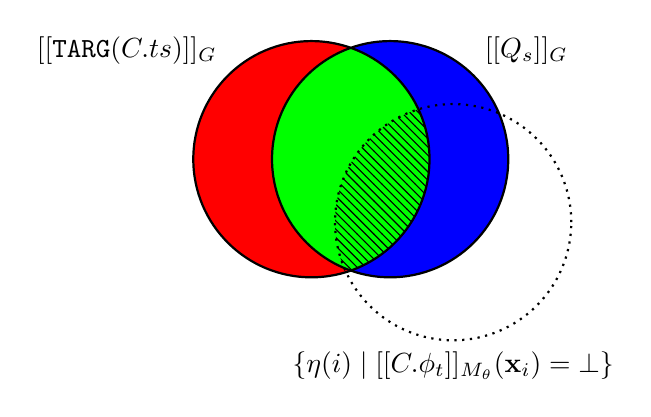
\begin{tikzpicture}[thick,
            set/.style = {circle,
                minimum size = 3cm}]
         
        % Set A
        \node[set,label={135:$[[\uri{TARG}(C.ts)]]_G$}] (A) at (0,0) {};
         
        % Set B
        \node[set,label={45:$[[Q_s]]_G$}] (B) at (1.0,0) {};
        
        % Set C
        \node[set, label={270:$\{\eta(i) \mid [[C.\phi_t]]_{M_\theta}(\mathbf{x}_i) = \bot\}$}] (C) at (1.8,-0.8) {};
        
        \fill[fill=red](0,0) circle(1.5cm);
        
        \fill[fill=blue](1.0,0) circle(1.5cm);
         
        % Intersection
        \begin{scope}
            \clip (0,0) circle(1.5cm);
            \clip (1.0,0) circle(1.5cm);
            \fill[fill=green](0,0) circle(1.5cm);
        \end{scope}
        
        \begin{scope}
            \clip (0,0) circle(1.5cm);
            \clip (1.0,0) circle(1.5cm);
            \clip (1.8,-0.8) circle(1.5cm);
            \fill[pattern=north west lines](0,0) circle(1.5cm);
        \end{scope}
         
        % Circles outline
        \draw (0,0) circle(1.5cm);
        \draw (1.0,0) circle(1.5cm);
        \draw[dotted] (1.8,-0.8) circle(1.5cm);
         
        % Set intersection label
        % \node at (0.5,0) {$B$};
        % \node at (-1.0,0) {$A$};
        % \node at (2.0,0) {$C$};
         
        \end{tikzpicture}
        \caption{Venn-Diagram visualizing the Different Kinds of Nodes Occurring during the Validation}   \label{fig:venn_diagram_showing_instances_to_reduce_during_shacl_validation}
\end{figure}



The entity validation function is called for every combination of a constraint $C$ and a node $\eta(i)$ related to a sample in the dataset. That is, the evaluation only requires the validation results for the nodes retrieved, when executing the seed query $Q_s$, used during creation of the dataset, over $G$ (in Figure \ref{fig:venn_diagram_showing_instances_to_reduce_during_shacl_validation} the right circle). Additionally, the algorithm only makes use of the entity validation function if the entity validation function contains the needed validation result. For a given constraint $C$ with a target shape, $C.ts$ this is only the case if the node is included in the target definition of the shape (left circle in Figure \ref{fig:venn_diagram_showing_instances_to_reduce_during_shacl_validation}). Finally, one can exploit the form of the constraint $C$ in the case of the 2-valued logic. Taking definition \ref{Def:constraint} and lemma \ref{S:3valueto2valuelogic} brings $C$ in the form \[\mathcal{S}\big|_{ts} \rightarrow \phi_{T}\] 
Because of the Boolean implication now used in $C$, if $[[C.\phi_t]]_{M_\theta}(\mathbf{x}_i)$ evaluates to true the whole constraint will also evaluate to true independent of the SHACL schema validation result generated for the evaluation of the left-hand side of the constraint (dotted circle in Figure \ref{fig:venn_diagram_showing_instances_to_reduce_during_shacl_validation}). 

As the entity validation function is created from a valid assignment, at most the validation results for the target nodes of the shapes in the shape schema are included, which are too many. This can be seen in Figure \ref{fig:venn_diagram_showing_instances_to_reduce_during_shacl_validation}. The area in blue represents the set of nodes originally not included in the target definition of the target shape. The red area, as well as the not dotted green area (in the case of the 2-valued logic), represent the nodes validated by the SHACL engine, although, the results are not needed by the validation engine to validate the constraints.

\begin{Satz}{Only Perform the SHACL Validation for Target Nodes Needed by the Validation Engine}{removeTargets}
    Given a constraint $C \in \mathbf{C}$ (as in definition \ref{Def:constraint}), a shape schema $\mathcal{S} = (S,\uri{TARG},\uri{DEF})$, a seed query $Q_s \in \mathbf{Q_T}$ used to retrieve the dataset $D$ and the sample-to-node mapping $\eta$ with problem instances $\mathbf{x}_i$ from a knowledge graph $G \in \mathbf{G}$,  the nodes needed to be validated by a SHACL engine to perform the constraint validation of $C$ can be limited to
    \begin{gather}
        H_2 = [[\uri{TARG}(C.ts)]]_G \cap [[Q_s]]_G \cap \{\eta(i) \mid [[C.\phi_t]]_{M_\theta(\mathbf{x}_i)} = \bot\} \label{2valuedlogicintersection}
    \end{gather}
    in case of the 2-valued logic (the dotted area marked in green in Figure \ref{fig:venn_diagram_showing_instances_to_reduce_during_shacl_validation}) or 
    \begin{gather}
    H_3 = [[\uri{TARG}(C.ts)]]_G \cap [[Q_s]]_G \label{3valuedlogicintersection}
    \end{gather} 
    in case of the 3-valued logic (the area marked in green in Figure \ref{fig:venn_diagram_showing_instances_to_reduce_during_shacl_validation}).     
\end{Satz}

Therefore, the goal is now to reduce the SHACL schema $C.\mathcal{S} = (S,\uri{TARG}, \uri{DEF})$ to a SHACL schema $\mathcal{S}' = (S',\uri{TARG'}, \uri{DEF})$, in such a way, that the validation results for the instances in $H_3$ resp. $H_2$ does not change. This can be formally expressed with
\begin{gather}
\forall G \in \mathbf{G} ~ \forall v \in H ~ \textit{validate}_\mathcal{S}(v,C.ts,G) = \textit{validate}_{\mathcal{S}'}(v,C.ts,G) \label{consistency_shape_shema}
\end{gather}
where $\textit{validate}_\mathcal{S}$ is the entity validation function for $\mathcal{S}$ and $H$ is $H_2$ or, $H_3$ depending on the logic used.

To remove the kind of instances validated unnecessarily by the SHACL engine, the target definition of the target shape $C.ts$ can be limited to the intersection $H$. Therefore, the seed query $Q_s$ is extracted from the dataset generating query $Q_D$ by only projecting $?x$:
\begin{gather}
    Q_s = \uri{SELECT}(?x,id, Q_D) \label{seed_query_from_dataset_generating_query}
\end{gather}
Next, in case of the 2-valued logic the nodes in the set $\{\eta(i) \mid [[C.\phi_t]]_{M_\theta}(\mathbf{x}_i) = \bot\}$ can be estimated by early evaluating the right-hand side of the constraint and making use of the sample-to-node mapping $\eta$. Given the IRIs of the nodes, a filter condition $R$ can be built to restrict the validation to these nodes. In the case of the 3-valued logic, it holds $R = \top$.

Both $Q_s$ and $R$ can now be used in the target definition of the target shape $C.ts$ of the reduced shape schema:
\[
    \uri{TARG'}(s) =    \begin{cases} 
                            \uri{TARG}(s) & s \neq C.ts\\
    \uri{SELECT}(?x,id,((Q_s \uri{ AND } \uri{TARG}(C.ts)) \uri{ FILTER } R)) & \text{else}
                        \end{cases}
\]
Clearly, the change of \uri{TARG}(C.ts) does not affect formula \ref{consistency_shape_shema}.

The execution of the SHACL engine over a shape schema, as performed in line \ref{algo:validation_engine:shaclEngine}, produces \emph{at most} the validation results for the target nodes of the shapes in the shape schema. However, the evaluation of a constraint only needs the SHACL validation results for the shape $C.ts$ and further results should only be produced because of inter-shape constraints.

This is the second kind of instances validated unnecessarily by the SHACL engine. These shapes can be identified by taking the shape schema $\mathcal{S}$ as a directed graph, as defined below:

\begin{Def}{Dependency Graph of a Shape Schema \cite{figuera2021trav}}{}
    Given a shape schema, $\mathcal{S} = (S,\uri{TARG},\uri{DEF})$ the directed dependency graph $\Phi_\mathcal{S}$ is a tuple $(V_{\Phi_\mathcal{S}}, E_{\Phi_\mathcal{S}})$ with \[V_{\Phi_\mathcal{S}} = S\] and \[E_{\Phi_\mathcal{S}} = \{(s_i, s_j) \mid s_j \textrm{ appears in } \uri{DEF}(s_i)\}\]
\end{Def}

Given, $\Phi_\mathcal{S}$ one can identify the needed shapes $S'$ to be the ones reachable from $C.ts$. This is valid as the criterion $\uri{DEF}(C.ts)$ can still be evaluated as before because formula \ref{consistency_shape_shema} stays unaffected.

\begin{Satz}{Remove unneeded Shapes from the Shape Schema}{removeShapes}
    Given a constraint $C \in \mathbf{C}$ (as in definition \ref{Def:constraint}) and a shape schema, $\mathcal{S} = (S,\uri{TARG},\uri{DEF})$ the shapes to evaluate $C$ can be limited to the shapes, which are reachable from $C.ts$ in the directed dependency graph $\Phi_\mathcal{S}$.
\end{Satz}

Algorithm \ref{algo:reduced_shacl_validation} makes use of the two lemmas and is a replacement for $\mathbf{performShaclValidation}$ (line \ref{algo:validation_engine:performShaclValidation} in algorithm \ref{algo:validation_engine}). Additionally, the algorithm takes care of shape schemas used by multiple constraints. Taking multiple constraints into consideration is important as each shape schema should only be validated once over the knowledge graph, to avoid the redundant generation of SHACL schema validation results for shapes occurring in multiple reduced shape schemas. 
\begin{Satz}{Simultaneous Generation of SHACL Schema Validation Results for Constraints using the Same Shape Schema}{simulataneous_constraint_validation}
Given a set of constraints $\mathcal{C} \subset \mathbf{C}$ the SHACL schema validation results for all $\mathcal{C}_\mathcal{S} \in \mathcal{P}(\mathcal{C})$ for which all $C_i, C_j \in \mathcal{C}_\mathcal{S}$ imply $C_i.\mathcal{S} = C_j.\mathcal{S}$ should be generated simultaneously. 
\end{Satz}

However, lemmas \ref{S:removeTargets} and \ref{S:removeShapes} can both be extended easily to multiple constraints.
A group of constraints using the same shape schema $\mathcal{S}$, but different target shapes $ts_i$ ($i \in [1,2,...]$), needs for evaluation all shapes reachable from the $ts_i$ (lines \ref{algo:reduced_shacl_validation:reachableShapesStart} - \ref{algo:reduced_shacl_validation:reachableShapesEnd}). These are stored in \textit{relevantShapes}. In the next steps, for each shape schema occurring in the constraints (line \ref{algo:reduced_shacl_validation:EachShapeSchema}), a subset of the target shapes must be selected for which the target definition can be reduced (lines \ref{algo:reduced_shacl_validation:subset_selection_start} - \ref{algo:reduced_shacl_validation:subset_selection_end}). That is the target definition of a target shape $ts$, involved in the evaluation of another target shape $ts'$ may not be reduced, because the nodes $[[\uri{TARG}(C.ts)]]_G \setminus [[Q_s]]_G$ may be needed to evaluate $ts'$. In case the target definition of a target shape can be reduced, the filter condition used to further reduce the nodes in the target definition is computed per target shape. To avoid the evaluation of the right-hand side of the constraints, the SHACL validation needs to be performed interleaved with the constraint evaluation. Here for reasons of simplicity, line  \ref{algo:reduced_shacl_validation:filter_condition} can be thought of an oracle giving the correct filter condition.
Finally, the SHACL engine can be run on the reduced shape schema $\mathcal{S}'$ consisting of the updated target definitions $\uri{TARG}$ and the shapes $S'$ relevant for evaluation of the target shapes $ts_i$ (line \ref{algo:reduced_shacl_validation:runShaclEngine}).
\begin{algorithm}[H]
    \caption{Pseudocode of the Reduced SHACL Validation}\label{algo:reduced_shacl_validation}
    \begin{algorithmic}[1]
         \Function{reducedSHACLValidation}{Constraints $\mathcal{C}$, Query $Q_D$, Knowledge Graph $G$}
            \State $\textit{schemasForConstraints} \gets \emptyset$ \Comment{the list of constraints using the same shape schema}            
            \State $\textit{relevantShapes} \gets \emptyset$ \Comment{the needed shapes per shape schema} \label{algo:reduced_shacl_validation:reachableShapesStart}
            \State $\textit{involvedShapes} \gets \emptyset$ \Comment{the shapes involved when evaluating a constraint}
            \State $Q_s = \uri{SELECT}(?x,id, Q_D)$ \Comment{id is the identity function}
            \ForEach{$C \in \mathcal{C}$} 
                \State $\Phi_{C.\mathcal{S}} \gets \textbf{createDependencyGraph}(C.\mathcal{S})$
                \State $\textit{involvedShapes}[C] \gets \textbf{DFS}(\Phi_{C.\mathcal{S}}, C.ts)$
                \State $\textit{relevantShapes}[C.\mathcal{S}] \gets \textit{relevantShapes}[C.\mathcal{S}] \cup \textit{involvedShapes}[C]$
                \State $\textit{schemasForConstraints}[C.\mathcal{S}] = \textit{schemasForConstraints}[C.\mathcal{S}].\mathbf{append}(C)$
            \EndFor \label{algo:reduced_shacl_validation:reachableShapesEnd}
            \State $\textit{validate} \gets \emptyset$
            \ForEach{$\mathcal{S} \in \textit{schemasForConstraints}$} \label{algo:reduced_shacl_validation:EachShapeSchema}
                \State $\uri{TARG} \gets \mathcal{S}.\uri{TARG}$
                \ForEach{$C \in \textit{schemasForConstraints}[\mathcal{S}]$} \label{algo:reduced_shacl_validation:subset_selection_start}
                    \If{$C.ts \not\in \bigcup_{c \in \textit{schemasForConstraints}[\mathcal{S}] \setminus \{C\}} \textit{involvedShapes}[c]$} 
                        \State $R \gets \textbf{getFilterConditionForConstraint}(C)$ \label{algo:reduced_shacl_validation:filter_condition}
                        \State $\uri{TARG}(C.ts) \gets \uri{SELECT}(?x,id,((Q_s \uri{ AND } \uri{TARG}(C.ts)) \uri{ FILTER } R))$
                    \EndIf
                \EndFor \label{algo:reduced_shacl_validation:subset_selection_end}
                \State $\textit{validate}[\mathcal{S}] \gets \mathbf{runShaclEngine}((\textit{relevantShapes}[\mathcal{S}],\uri{TARG}, \mathcal{S}.\uri{DEF}), G)$ \label{algo:reduced_shacl_validation:runShaclEngine}
            \EndFor
            \State \Return{$\textit{validate}$}
        \EndFunction
    \end{algorithmic}
\end{algorithm}
        
        \subsection{How to Join the SHACL Validation Results with the Dataset}
            \label{section_executing_the_join}
            In the complexity analysis of the \textbf{evaluateConstraints} function in algorithm \ref{algo:validation_engine}, it is assumed that all the validation results fit into the main memory and, therefore, a hash table can be used to access the SHACL validation results in one step. However, this might not be the case, when a large dataset with many seed nodes combined with various constraints should be handled. 

This problem can be tackled by taking the different components involved as relations in a relational schema, which in turn allows using appropriate physical operators known from relational databases. First, there is the sample-to-node mapping $\eta$ and the dataset $D$ retrieved from a knowledge graph $G$. These two can be handled as one relation $T$(\underline{idx}, node\_id, x, y). Each entity of $T$ represents a sample $(\mathbf{x_i},y_i)$ in $D$ with the corresponding node\_id $\eta(i)$, identified by an index $i$ ($i \in [1,...,N]$ and $N$ the number of samples in $D$). Next, each SHACL validation corresponding to a constraint $C_j \in \mathcal{C}$ of a schema $\mathcal{S}_j$ with target shape $ts_{j,k}$ yields a relation $S_{j,k}$(\underline{node\_id}, $\textrm{result}_{j,k}$), where $j \in [1,...,m]$; $k \in [1,...,|\mathcal{S}_j.S|]$) and $m = |\mathcal{C}|$ the number of constraints. The entities of $S_{j,k}$ represent the SHACL validation results \textit{validate}(node\_id, $ts_{j,k}$, $G$) for each seed node identified by a $\textrm{node\_id} \in [[\mathcal{S}_j.\uri{TARG}(ts_{j,k})]]_G$.

During the evaluation of the constraints for each sample in the dataset, the SHACL validation results are needed, which expresses the need for the relations joined with respect to the seed nodes respectively the node identifiers. While performing the join, special attention to the $S_{j,k}$ relations is required as there will be node identifiers without a SHACL validation result for some $j,k$ as only nodes in the corresponding target definition of the target shape are handled. Therefore, outer-joins must be used to retain all dataset indices and validation results. Restricting the selection of query execution trees to left-deep trees yields two different join strategies, which are depicted in Figure \ref{fig:join_strategies_left_deep}.

\begin{figure*}
    \centering
    \begin{subfigure}[b]{0.4\textwidth}
            \centering
            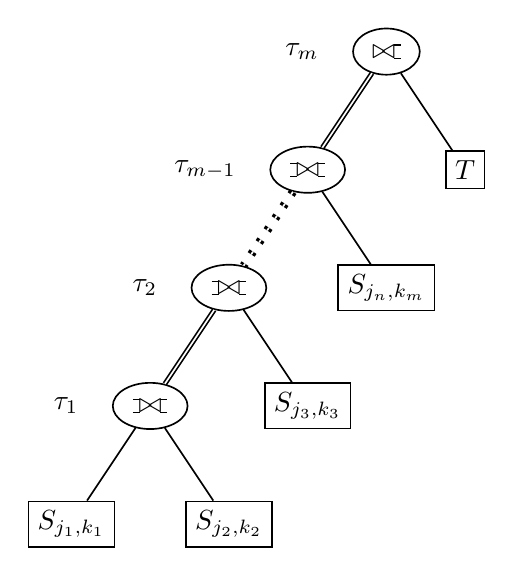
\begin{tikzpicture}[
            style = {sibling distance = 2cm, semithick}]
            \node (t1) [draw,ellipse]{$\rightouterjoin$}
                child {node (t2) [draw, ellipse, solid, semithick] {$\fullouterjoin$} edge from parent [solid, semithick, double]
                    child {node (t3) [draw, ellipse, solid, semithick] {$\fullouterjoin$} edge from parent [loosely dotted, very thick, double]
                        child {node (t4) [draw, ellipse, solid, semithick] {$\fullouterjoin$} edge from parent [solid, semithick, double]
                            child {node [draw,solid,semithick] {$S_{j_1,k_1}$} edge from parent [solid,semithick]}
                            child {node [draw,solid,semithick] {$S_{j_2,k_2}$} edge from parent [solid,semithick]}
                        }
                        child {node [draw, solid, semithick] {$S_{j_{3},k_{3}}$} edge from parent [solid, semithick]} 
                    }
                    child {node [draw, solid, semithick] {$S_{j_{n},k_{m}}$} edge from parent [solid, semithick]} 
                }
            child {node [draw, solid, semithick] {$T$} edge from parent [solid, semithick]};
            \node[left=0.3cm of t1] {$\tau_m$};
            \node[left=0.3cm of t2] {$\tau_{m-1}$};
            \node[left=0.3cm of t3] {$\tau_2$};
            \node[left=0.3cm of t4] {$\tau_1$};
            \end{tikzpicture}    
            \caption{Join T at the end}
            \label{fig:join_strategies_left_deep1}
    \end{subfigure}
    \begin{subfigure}[b]{0.4\textwidth}
            \centering
            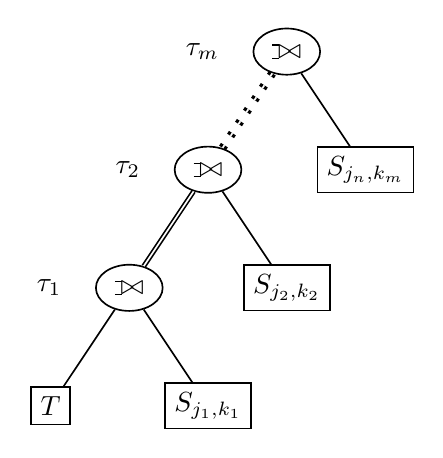
\begin{tikzpicture}[
            style = {sibling distance = 2cm, semithick}]
            \node (t1)[draw,ellipse]{$\leftouterjoin$}
                child {node (t2) [draw, ellipse] {$\leftouterjoin$} edge from parent [loosely dotted, very thick, double]
                    child {node (t3) [draw, ellipse, solid, semithick] {$\leftouterjoin$} edge from parent [solid, semithick, double]
                        child {node [draw, solid, semithick] {$T$} edge from parent [solid, semithick]}
                        child {node [draw, solid, semithick] {$S_{j_1,k_1}$} edge from parent [solid, semithick]}
                    }
                    child {node [draw, solid, semithick] {$S_{j_2,k_2}$} edge from parent [solid, semithick]} 
                }
                child {node [draw, solid, semithick] {$S_{j_{n},k_{m}}$} edge from parent [solid, semithick]
            };
            \node[left=0.3cm of t1] {$\tau_m$};
            \node[left=0.3cm of t2] {$\tau_2$};
            \node[left=0.3cm of t3] {$\tau_1$};
            \end{tikzpicture}
            \caption{Join T at the beginning}
            \label{fig:join_strategies_left_deep2}
    \end{subfigure}
    \caption{Execution Trees with Intermediate Results $\tau$ and Double Lines Denoting Pipelining}
    \label{fig:join_strategies_left_deep}
\end{figure*}

In the present context, applying the reductions from section \ref{section_shaclapi} when possible, it can be seen that the following equations hold:
\begin{gather}
    |T| = |[[Q_D]]_G| = |D| \label{eq:size_t}\\
    |S_{j,k}| = |[[\mathcal{S}_j.\uri{TARG}(ts_{j,k})]]_G| \label{eq:size_s}\\
    |\tau \fullouterjoin S_{j,k}| = |\pi_{\textrm{node\_id}}(\tau) \cup \pi_{\textrm{node\_id}}(S_{j,k})| \geq |S_{j,k}|, |\tau| \label{eq:join_s}\\
    |T \leftouterjoin \tau| = |\tau \rightouterjoin T| = |T| \geq |\tau| \label{eq:join_t}
\end{gather}
where $\tau$ denotes an arbitrary intermediate result occurring in the execution trees. 

Formula \ref{eq:join_t} is conceptually more involved, that is why it is proved below:
\begin{proof}
Each part of the equation can be proved on its own:

\textbf{1.)} $|T \leftouterjoin \tau| = |\tau \rightouterjoin T|$ is true for all possible relations $T$ and $\tau$ because of symmetry.

\textbf{2.)} $|\tau \rightouterjoin T| = |T|$ is proved by reasoning over $\tau_j$ ($l \in [1,...,m]$) given the execution trees in Figure \ref{fig:join_strategies_left_deep}. 

In case of Figure \ref{fig:join_strategies_left_deep1}, it is $\tau_1 = (S_{j_1,k_1} \fullouterjoin S_{j_2,k_2})$ and $\tau_l = (\tau_{l-1} \fullouterjoin S_{j_{(l+1)},k_{(l+1)}})$. We note that for each $S_{j,k}$ the \textrm{node\_id} is unique. Therefore the \textrm{node\_id} will be unique for all $l$ in $\tau_l$. $T$ contains all $node\_id$'s which can occure at least once (see lemma \ref{S:removeTargets}); implying $\forall l ~ \pi_{\textrm{node\_id}}(\tau_l) \subseteq \pi_{\textrm{node\_id}}(T)$. This is sufficient for $\forall l ~ |\tau_l \rightouterjoin T| = |T|$ to be true in case of Figure \ref{fig:join_strategies_left_deep1}.

In case of Figure \ref{fig:join_strategies_left_deep2}, it is $\tau_1 = (T \leftouterjoin \mathcal{S}_{j_1,k_1})$ and $\tau_l = (\tau_{l-1} \leftouterjoin S_{j_l,k_l})$. With the argumentation as above we can see that $\forall l ~ \pi_{\textrm{node\_id}}(\mathcal{S}_{j_l,k_l}) \subseteq \pi_{\textrm{node\_id}}(T)$. Clearly $\pi_{\textrm{node\_id}}(\tau_1) = \pi_{\textrm{node\_id}}(T)$ applies and $\forall l ~ \pi_{\textrm{node\_id}}(\tau_l) = \pi_{\textrm{node\_id}}(T)$ follows by induction over $l$. Again, this is sufficient for $\forall l ~ |\tau_l \rightouterjoin T| = |T|$ to be true in case of Figure \ref{fig:join_strategies_left_deep2}.

\textbf{3.)} $|T| \geq |\tau|$ can be proved with the same arguments as $\textbf{2.)}$.
\end{proof}

Equations \ref{eq:size_t} and \ref{eq:size_s} put the cardinality of the relations in the context of the validation engine. That is, the cardinality of $T$ is equal to the cardinality of the dataset retrieved from the given knowledge graph and the cardinality of $S_{j,k}$ is equal to the number of nodes included in the target definition of $ts_{j,k}$.

Next, both execution plans in Figure \ref{fig:join_strategies_left_deep} are analyzed separately using the cost model in Table \ref{fig:physical_operators_join} with respect to the order in which the $S_{j,k}$ relations are best joined and which execution plan should be chosen.

\begin{table}
    \centering
    \begin{tabular}{p{3cm}|p{5cm}|p{5cm}}
        \toprule
        physical operator for $R \substack{\bowtie\\A=B} S$ & requirements & read cost\\
        \midrule
        \midrule
        Index join & Index on $B$ in $S$ and $B$ is unique in $S$ & $|R| + |R| (k + log(\#(B,S)))$ where $k$ denotes the average number of $B$ matches in $S$ given the $A$ values from $R$.\tablefootnote{$\#(B,S)$ denotes the number of different $B$ values in $S$}\\
        Sort join & $R$ and $S$ are sorted w.r.t A resp. B & $|R| + |S|$\\
        Hash join & Requires $S$ to match into memory, in one or vertical partitioned & $|R| + |S|$\\
        \bottomrule
    \end{tabular}
    \caption{Simplified Cost Model for Different Physical Join Operators}
    \label{fig:physical_operators_join}
\end{table}

\paragraph{a) Join T at the end} With the equations \ref{eq:join_s} and \ref{eq:join_t} it follows that during the execution of the operation tree the intermediate results are increasing monotonously up to $|T|$. 

In case of the index join, the cost can be approximated to be:
\begin{align*}
    & \underbrace{|\tau_{m-1}| + |\tau_{m-1}| * \left(\frac{|T|}{\#(\textrm{node\_id}, T)} + log(\#(\textrm{node\_id}, T))\right)}_{\textrm{read cost $\rightouterjoin$}}\\  
    & + \underbrace{\sum_{i=0}^{m-2} \left[ |\tau_i| * (2 + log(\#(\textrm{node\_id}, S_{j_{i+2},k_{i+2}}))\right]}_{\textrm{read cost $\fullouterjoin$}} + \underbrace{|\tau_m| - \sum_{i=1}^{m-1} \left[|\tau_i|\right]}_\textrm{write cost - pipelining}\\
    &= |\tau_{m-1}| * \left(\frac{|T|}{|[[Q_s]]_G|} + log(|[[Q_s]]_G|)\right) + \sum_{i=0}^{m-2} \left[ |\tau_i| * (1 + log(|S_{j_{i+2},k_{i+2}}|))\right] + |T| + |\tau_0|
\end{align*}
where $\tau_0 = S_{j_{1},k_{1}}$, $|\tau_m| = |T|$, and the node\_ids are unique for all $S_{j,k}$ and in each $\tau_i$. Therefore, to simplify the calculation, the $k$ in the formula for the read cost of the index join is set to $1$, when joining with a $S$. In the join with, $T$ it is used that the node\_ids in $T$ correspond to the seed nodes in the sample-to-node mapping, which can be retrieved with the $Q_s$ generated with equation \ref{seed_query_from_dataset_generating_query}.

In case of the sort or the hash join, the cost can be approximated to be:
\begin{align*}
    & \underbrace{(|\tau_m-1| + |T|) + \sum_{i=0}^{m-2} \left[|\tau_i| + |S_{j_{i+2},k_{i+2}}|\right]}_{\textrm{read cost}} + \underbrace{\sum_{i=1}^{m} \left[|\tau_i|\right]}_\textrm{write cost}
\end{align*}
where $\tau_0 = S_{j_{1},k_{1}}$ and $|\tau_m| = |T|$.
However, these types of joins do not support pipelining as the final result is written multiple times until the final result is ready. The sort join comes with the additional requirement of sorted input relations, adding a cost in the order of $O(m * |T|*log(|T|))$.

Therefore, considering the cost complexity of the physical join operators, the following heuristic to minimize the cost arises:

\begin{Satz}{Join-Heuristic 1}{join_heuristic1}
When joining $T$ at the end, the $j_1,...,j_m$ and $k_1,...,k_m$ in Figure \ref{fig:join_strategies_left_deep1} should be chosen such that the cardinality of the intermediate results $\tau_1,...,\tau_{m-1}$ are as small as possible.
\end{Satz}

One might think about converting the left-deep execution tree into a right-deep execution tree to reduce the cost\footnote{Assuming $|\tau_i| > |S_{j_{i+2},k_{i+2}}|$ for enough $i$'s} to:
\begin{multline*}
    \underbrace{|T| * (2 + log(\#(\textrm{node\_id}, \tau_{m-1}))) + \sum_{i=0}^{m-2} \left[ |S_{j_{i+2},k_{i+2}}| * (2 + log(\#(\textrm{node\_id}, \tau_i))\right]}_{\textrm{read cost}} \\
    + \underbrace{|\tau_m| - \sum_{i=1}^{m-1} \left[|\tau_i|\right]}_\textrm{write cost - pipelining}
\end{multline*}
where the $k$ in the index join is again set to $1$, assuming the maximal number of matches, when joining with an intermediate result $\tau_i$.
However, this involves maintaining the index structure of the intermediate results. Assuming a b-tree is used for indexing, this would yield an additional cost in the size of $O(|T| * log(|T|))$, which might lead to a worse execution time.

\paragraph{b) Join T at the beginning} The execution plan leads to a constant cardinality of the intermediate results of $|T|$ right from the beginning (see \ref{eq:join_t}).
Therefore, the cost calculation will be analog to the last paragraph but with the difference that all $|\tau_i|$ are as worse as possible, i.e., $|T|$. Further, an index structure over the node\_ids in $T$ will be useful as it can be used in every step of the execution plan. 
On the good side, it allows joining the SHACL validation results incrementally with $T$ and, therefore, interleaving the join and the SHACL validation will yield usable results right after the first SHACL schema is validated, and the results are joined.

\begin{Satz}{Join-Heuristic 2}{join_heuristic2}
$T$ should be joined in the end or as early as intermediate SHACL validation results in combination with the dataset indices are needed.
\end{Satz}
        
        \subsection{Performing SHACL Constraint Validation during SPARQL Query Execution}
            \label{section_valSPARQL}
            
    Although validation of a knowledge graph builds on querying, when performed over a SPARQL endpoint, the sections \ref{background_sparql} and \ref{background_shacl} introduced querying and validating a knowledge graph as two different concepts. This section presents the concept of validating SHACL constraints during SPARQL query execution as proposed by Rohde et al. \cite{valSPARQL} as a possibility to improve the validation engine in algorithm \ref{algo:validation_engine}.
    Originally, SHACL constraint validation is done during SPARQL query execution to ``... [increase] the explainability of SPARQL query results by annotating them with information from the SHACL shape schema validation.`` \cite{valSPARQL}.
    Here the inspection of algorithm \ref{algo:validation_engine} shows that the SHACL schema is evaluated over the knowledge graph (line \ref{algo:validation_engine:shaclEngine}) and afterwards combined (lines \ref{algo:validation_engine:start_eval} - \ref{algo:validation_engine:end_eval}) with the query results retrieved before (line \ref{algo:validation_engine:dataset}).
    As shown by Rohde et al., performing both task simultaneously allows to repeatedly exploit the knowledge encoded in the SPARQL query like shown in section \ref{section_shaclapi}.
    
    Next, the notation from section \ref{background_sparql} is extended to perform the SHACL validation from section \ref{background_shacl} during query execution. Afterward, the pseudocode used to repeatedly exploit the knowledge encoded in the seed query $Q_s$ is presented.
    
    In comparison to the notation introduced in \cite{valSPARQL}, the concept of the explanation and the solution mapping is decoupled in a first step and instead there is an explanation function, which is able to map the needed validated RDF terms to a set of validation results. 
    
    \begin{Def}{Explanation Mapping}{valSPARQL_explanation} 
        An explanation mapping $E$ is a partial function, which maps an RDF term $t \in (\mathbf{B} \cup \mathbf{L} \cup \mathbf{I})$ to a set of validation results for that term. A validation result consist of the shape $s \in \mathbf{S}$ against which the node is validated and the validation result, which can be valid ($\top$) or invalid ($\bot$). Therefore it's
        \begin{gather*}
            E: \mathbf{B} \cup \mathbf{L} \cup \mathbf{I} \to \mathcal{P}(\mathbf{S} \times \{\top, \bot\})
        \end{gather*}
        Two explanation mappings $E_1$ and $E_2$ can be united via $E_1 \cup E_2$ by merging the partial functions as follows:
        \begin{gather*}
            E_1 \cup E_2 = \{(t \mapsto E_1(t) \cup E_2(t)) \mid t \in (\mathbf{B} \cup \mathbf{L} \cup \mathbf{I})\}
        \end{gather*}
        where all unspecified values $t$ are assumed to have as default value the empty set.
        The infinite set of explanation mappings is denoted with $\mathbf{E}$.
    \end{Def}
    
    To annotate the query results, it is necessary to extend the notion of a set of solution mappings as introduced in section \ref{background_sparql} with the explanation defined above. 
    
    \begin{Def}{A modified valSPARQL Mapping Set}{valSPARQL_mapping_sets}
    A modified valSPARQL mapping set is a triple $(\Omega, E, sn)$ where $\Omega \subset \mathbf{M}$, $E \in \mathbf{E}$ and $sn \in \mathbf{SN}$.
    \end{Def}    
    
    As in section \ref{background_sparql} several algebraic operations over the solution sets need to be defined. The solution sets are now modified valSPARQL mapping sets instead of sets of SPARQL solution mappings.
     
    \begin{Def}{Algebraic Operations over Modified valSPARQL Mapping Sets}{valSPARQL_algebra}
        Given two modified valSPARQL mapping sets $F_1 = (\Omega_1, E_1, sn_1)$ and $F_2 = (\Omega_2, E_2, sn_2)$, a set of variables $v \subset \mathbf{V}$, a filter condition $R$ and a function used for renaming of variables $\mathcal{r}:\mathbf{V} \to \mathbf{V}$ the following operations are defined:
        \begin{center}
            \begin{tabular}{l|l|l|l}
                \toprule
                operation & $\Omega$ & $\mathcal{G}_E$ & $sn$\\
                \midrule
                \midrule
                $\pi_v(F_1)$ & $\pi_v(\Omega_1)$ & $\{(\mu(x) \mapsto E_1(\mu(x))) \mid x \in v \land \mu \in \Omega\}$ & $sn_1$\\
                $\sigma_R(F_1)$ & $\sigma_R(\Omega_1)$ & $\{(s \mapsto E_1(s)) \mid s \in \text{dom}(\mu) \land \mu \in \Omega \}$ & $sn_1$\\
                $F_1 \cup F_2$ & $\Omega_1 \cup \Omega_2$ & $E_1 \cup E_2$ & $sn_1 \cup sn_2$\\
                $F_1 \bowtie F_2$ & $\Omega_1 \bowtie \Omega_2$ & $E_1 \cup E_2$ & $sn_1 \cup sn_2$\\
                $F_1 \setminus F_2$ & $\Omega_1 \setminus \Omega_2$ & $\{(s \mapsto E_1(s)) \mid s \in \text{dom}(\mu) \land \mu \in \Omega \}$ & $sn_1$\\
                $\rho(\mathcal{r},F_1)$ & $\rho(\mathcal{r}, \Omega_1)$ & $E_1$ & $sn_1$ \\
                \bottomrule
            \end{tabular}
        \end{center} % TODO: Fix the table use \mathcal{G}_{EXP}
        Given the operation in the left most column, the result is a new valSPARQL mapping set $(\Omega, E, sn)$.
    \end{Def}
    
    The next step is to build the explanation mapping during SPARQL query evaluation. 
    
    This is done inductively over the graph pattern expressions and analog to definition \ref{Def:sparql_graph_pattern}. 
    Therefore, the induction starts with the evaluation of a triple pattern, which utilizes a modified version of the entity explanation function defined in \cite{valSPARQL}.
    \begin{Def}{Entity Explanation Function}{valSPARQL_explaination}
    The entity explanation function $\text{exp} : \mathbf{M} \times \mathbf{T} \times  \mathbf{SN} \times \mathbf{G} \to \mathbf{E}$ maps the substituted subject $s$ of a triple pattern $t$, given a mapping $\mu$ to an explanation mapping with respect to the matching shapes $sh \in S$ from a shape schema $sn = (S, \uri{TARG}, \uri{DEF})$ over a knowledge graph $G$. 
    \begin{align*}
        \text{exp}(\mu(t),t,sn,G) =  \{(s \mapsto & \{ (sh, \text{validate}(s,sh,G)) \mid\\ & sh \in S \land s \in [[\uri{TARG}(sh)]]_G\})\}
    \end{align*}
    where $s = \mu(t)[0]$
    \end{Def}
    
    Now the evaluation of a triple pattern with respect to a shape schema and a knowledge graph can be defined as
    
    \begin{gather*}
        [[t]]_G^{sn} = ([[t]]_G, \bigcup_{\mu \in [[t]]_G} \text{exp}(\mu(t), t, sn, G), sn)
    \end{gather*}
    
    The further steps of the induction stay the same as in definition \ref{Def:sparql_graph_pattern} but now use the algebraic operations over the modified valSPARQL mapping sets. Therefore, all occurrences of $[[P]]_G$ in definition \ref{Def:sparql_graph_pattern} need to be replaced with $[[P]]_G^{sn}$ where $sn \in \mathbf{SN}$, $P \in \mathbf{P}$ and $G \in \mathbf{G}$.
        This concludes the notation needed to perform SPARQL query execution during SHACL constraint validation.
    
    \begin{Def}{Execution of $Q$ over $G$ while validating w.r.t. $sn$}{valSPARQL_execution}
        The execution of the SPARQL \uri{SELECT} query $Q$ over the knowledge graph $G$ while validating w.r.t. a shape schema $sn$ is written as a function $[[Q]]_G^{sn}: \mathbf{Q} \times \mathbf{G} \times \mathbf{SN} \to \mathcal{P}(\mathbf{M}) \times \mathbf{E} \times \mathbf{SN}$ and gives a modified valSPARQL mapping set.
    \end{Def}
    
    Finally, to make up the decoupling in the beginning, the query results $\Omega$ can be joined with the modified valSPARQL explanation $E$ to get the annotated query results as in \cite{valSPARQL}:
    \begin{gather}
    \Omega \bowtie E = \{(\{(t, \mu(t)) \mid t \in \text{dom}(\mu)\}, \{(t,sh,val) \mid (sh, val) \in \text{E}(t) \land t \in \text{dom}(\mu)\} ) \mid \mu \in \Omega\} \label{join_mapping_set_validation_results}
    \end{gather}
    Clearly, this step might also be pushed down into the evaluation of the query, which would result in a slight change of definition \ref{Def:valSPARQL_algebra} to handle SPARQL mapping sets joined with the explanation mapping \cite{valSPARQL}. 
        
    The following describes the pseudocode of the valSPARQL approach (algorithm \ref{algo:valSPARQL}).
    The approach decomposes the given query $Q$ into so-called subject star-shaped queries (line \ref{algo:valSPARQL:decomp}), whose results are joined afterwards according to the algebraic operations (see definition 9 in \cite{valSPARQL}) (line \ref{algo:valSPARQL:overall_join}). A subject star-shaped query is a non-nested query consisting of the conjunction of triple patterns with the same subject \cite{vidal2010efficiently}. The pseudocode uses such a decomposition and additionally performs the join (equation \ref{join_mapping_set_validation_results}) per star-shaped query result mapping set (line \ref{algo:valSPARQL:join}). During the decomposition, for each star-shaped query, a shape $s$ is determined. This is done by associating each star-shaped query with a class of entities in the knowledge graph and inferring the shape in the shape schema associated with that class. 
    Besides performing SHACL validation during query processing, also the SHACL schema is reduced as described in section \ref{section_shaclapi} (lines \ref{algo:valSPARQL:reduction_start} - \ref{algo:valSPARQL:reduction_end}). 
    
    \begin{algorithm}[H]
    \caption{Pseudocode of the valSPARQL Approach}\label{algo:valSPARQL}
    \begin{algorithmic}[1]
    \Function{valSPARQL}{Query $Q$, Shape Schema $\mathcal{S}$, Knowledge Graph $G$} 
    	\State $\textit{plan} \gets \textbf{generateBushyExecutionPlan}(Q,\mathcal{S})$ \label{algo:valSPARQL:decomp} \Comment{$ssq$ is a star-shaped query}
    	\ForEach{$(ssq,s) \in \textit{plan}$} \Comment{$s$ is the shape chosen for $ssq$}
    	    \State $sn_i \gets \mathcal{S}$ \label{algo:valSPARQL:reduction_start}
    	    \State $\Phi_{sn_i} \gets \textbf{createDependencyGraph}(sn_i)$
            \State $sn_i.S \gets \textbf{DFS}(\Phi_{sn_i}, s)$
    	    \State $sn_i.\uri{TARG}(s) \gets \uri{SELECT}(?x,id,(ssq \uri{ AND } sn_i.\uri{TARG}(s)))$\label{algo:valSPARQL:reduction_end}
    	    \State $(\Omega_i, E_i, sn_i) \gets [[ssq]]_G^{sn_i}$
    	    \State $M_i \gets \Omega_i \bowtie E_i$ \label{algo:valSPARQL:join}
    	\EndFor
    	\State \Return{$\textbf{applyOperators}(\textit{plan},M_1,...)$} \label{algo:valSPARQL:overall_join}
    \EndFunction
    \end{algorithmic}
    \end{algorithm}
    
    The approach described in this section combines the process of the execution of a SPARQL query with the evaluation of a SHACL schema over a knowledge graph. In the validation engine (algorithm \ref{algo:validation_engine}) the dataset constructing query $Q_D$ is executed without evaluating a SHACL schema. However, the constraints $\mathcal{C}$ are already known and, therefore, one may decide to early evaluate a SHACL schema $\mathcal{S}$ coming from a set of constraints $C \subset \mathcal{C}$ with the target shapes $ts_i$ ($i \in [1,2,...]$) matching the shapes $s$ assigned to the star-shaped queries.
    
    
    
    % Explain the architecture 
    
    % \begin{figure}
    %     \centering
    %     \includegraphics[width=\textwidth]{images/valSPARQL/valSPARQL.png}
    %     \caption{valSPARQL architecture}
    % \end{figure}

    %In general the motivation is twofold. First of all it's something, which is closely related to relational databases. Integrity constraints are defined and checked by the engine (for example a SQL engine) to keep the answers to queries and also the whole database consistent. When querying a possible automated generated knowledge graph, there also might be integrity constraints (then called a shape schema) which should be validated, when accessing the related data. This will then lead to increased explainability of SPARQL query results through annotations with SHACL shape schema validation reports.
    %In the second place with state-of-the art query engines to get validated query results, one would need to evaluate the complete SHACL schema over the graph and then combine the query results with the validation report. Performing both things in parallel leads to space during validation to exploiting the knowledge encoded in the SPARQL query. \cite{valSPARQL}


        \subsection{Different Types of Constraints}
            \label{section_further_types_of_constraints}
            In definition \ref{Def:constraint} a constraint is defined to be of a specific form, which makes use of a SHACL shape schema associated with a target shape as a condition and a logical expression about the predicted target as a restriction. This kind of constraint can be used during inference to explain and check the model's predictions. When the condition of the constraint applies to the problem instance and its semantic context in the knowledge graph, the validation result grades the prediction made by the model to be correct or incorrect according to the constraint. If the validation result confirms the model's prediction, the constraint gives an explanation for the prediction. If the prediction turns out to be incorrect, the result might be used to identify the reason for that. However, in both cases, the explanation or the reasoning is only necessarily true if the underlying knowledge graph is correct. Given the application, this kind of constraint is now referred to as \emph{prediction constraint}. 

\begin{Def}{Prediction Constraint}{prediction_constraint}
The type of constraint as defined in definition \ref{Def:constraint}, which, when evaluated over a machine learning model given the underlying knowledge graph and the sample-to-node mapping, makes a statement about the correctness of the predictions of the model, by assuming a correct data basis is called prediction constraint. 
\end{Def}

This is in contrast to a constraint, which does not take into consideration the predictions of the model. As no statement is made about the truth of the model's predictions, the constraint validation results are only about the integrity of the semantic data in the knowledge graph. It is the samples in the dataset, which are now validated or invalidated with respect to the semantic context given in the knowledge graph. Therefore, each constraint validation result measures the trustworthiness of the sample in the dataset.

Clearly, there are different possibilities to represent such a constraint. In some cases, it might be enough to mark the $i$th sample as valid/invalid if the associated node $\eta(i)$ is retrieved by a SPARQL query and else as invalid/valid. However, using a SHACL shape schema $\mathcal{S} = (S,\uri{TARG}, \uri{DEF})$ to represent constraints over a knowledge graph is the W3C recommended approach and is at least as expressive as a SPARQL query (see below). The definition is done analog to a prediction constraint, but only uses the condition part of the implication.

\begin{Def}{Data Constraint}{data_constraint}
A constraint $C \in \mathbf{C}$ is called a data constraint if the constraint only measures the trustworthiness of the samples in the dataset, by looking at their feature values and their semantic context given in the knowledge graph.

Here every data constraint $C$ is composed of a shape schema $\mathcal{S} = (S, \uri{TARG}, \uri{DEF})$ ($\mathcal{S} \in \mathbf{SN}$) and a target shape $ts \in S$. The constraint is serialized as follows:
\[\mathcal{S}\big|_{ts}\] 
The components of $C$ can be accessed with $C.\mathcal{S}$ and $C.ts$.
\end{Def}

To stay with the 3-valued logic and the notation known from the prediction constraints, a data constraint $C$ is evaluated with respect to a knowledge graph $G$ and the node $\eta(i)$, that uses the sample-to-node mapping $\eta$ applied to the $i$'th sample in a dataset, using the Scott-brackets:

\begin{gather}
    [[C_d]]_{G,\eta(i)} = \begin{cases} \text{validate}(\eta(i),ts,G) & \eta(i) \in [[\uri{TARG}(ts)]]_G\\ -1 & \text{else}
    \label{F:constraint_data} \end{cases}
\end{gather}

Using the 3-values logic comes with the benefits of more detailed validation results. Precisely, a data constraint only applies to a seed node and the associated sample, when the seed node is included in the target definition of the specified target shape of the constraint. If a data constraint labels a sample as valid or invalid, that is because the shape applies or does not apply to the related seed node.

For example, a data constraint $C_{Q}$ can be used to mark the instances retrieved by a query $Q$ as 'valid' ($1$) and the rest as 'not applicable' $-1$, by setting $C_{Q}.\mathcal{S} = (\{s_1\}, \{s_1 \mapsto Q\},\{\})$.
The example shows that using SHACL for data constraints is at most as expressive as a constraint, which would only be based on a SPARQL query.

Again, the 3-valued logic can be transformed into the 2-valued logic by taking the absolute value. However, the transformation may lead to misleading results as it might be the case that every sample seems to be valid, although, in fact, not a single sample was validated.

Further, the transformation shows the similarity of the left-hand side $\mathcal{S}\big|_{ts}$ of a prediction constraint defined in definition \ref{Def:constraint} with a \emph{data constraint} C: 
\begin{gather}
    \left|[[C]]_{G,\eta(i)}\right| = [[\mathcal{S}\big|_{ts}]]_{G,\eta(i)} \label{data_prediction_shape_evaluation_comp}
\end{gather}

Although the validation results of a data constraint only make a statement about the validity of the samples in the dataset and not the predictions of the model, for notation convenience both will be saved by the validation engine in the model-validation-result function $\Theta$ as defined in definition \ref{Def:model_validation_result_function}.

Adopting the $\textbf{evaluateConstraints}$ function in algorithm \ref{algo:validation_engine} to different types of constraints is a matter of differentiating between the types. When evaluating a data constraint line \ref{algo:validation_engine:constraintLeftValidateDefault} needs to assign $-1$ and lines \ref{algo:validation_engine:constraintRight} - \ref{algo:validation_engine:end_combine} can be replaced with \[\mathcal{G}_\Theta \gets \mathcal{G}_\Theta \cup \{(C,i) \mapsto \textit{left}\}\] This change does not change the complexity of the validation engine as evaluating the right-hand side of the prediction constraint in combining the results was assumed to take constant time.

% TODO: Converting a prediction constraint into a data constraint by using the ground truth values.

% TODO: Example: e.g. only females can be pregnant -> male persons can not be pregnant
    
    \section{Constraint-based Explanations and Interpretations}
        \label{section_constraint_based_explanations}
        In this section, the focus is on using the validation results available as model-validation-result function $\Theta$ to get insights into the model behavior (see lemma \ref{S:problem_explaining_ai_model_with_constraints}) and explain predictions made by the model, when possible. $\Theta$ was generated by validating the model $M_\theta$ and the samples extracted from a knowledge graph $G$ with user-defined prediction and data constraints. Because of the different semantics as explained in section \ref{section_further_types_of_constraints} different usage scenarios arise:

\begin{enumerate}
    \item Training a model, which conforms to specific requirements
        \begin{enumerate}
            \item Understand the influence of bad data (w.r.t. data constraints) used to train the model 
            \item Analyze why the model may have made bad decisions w.r.t. prediction constraints
        \end{enumerate}
    \item During the model inference explain a model prediction made based on a problem instance w.r.t. prediction constraints
\end{enumerate}

These scenarios are relevant for different kind of users. The machine learning engineer is interested in creating models, which conform to requirements of the client and have as less errors as possible. In that case, the explanations can be used to gain insights into the model behavior (scenario 1), which then might be used to improve the model. For example, through changing the hyperparameters of the model, being able to perform further data cleansing or further feature engineering. The next group of people are the ones offering the model to the world. For them it is important to have a model, which makes predictions conforming to governmental regulations, or scientific facts (e.g., medical or physical) and social principles. As they are not interested in improving the model directly, but instead want to see that the model they are selling is correct (scenarios 1b and 2). Finally, there are the users of the model. As a user, one wants to be able to justify the decision made by the model and one might have certain constraints on the model, which should be respected and can be used to explain the predictions made by the model (scenario 2). In this thesis, a graphical approach is used for explanations, as this is meant to facilitate the understanding of the model by the different kinds of user groups and can be interpreted properly according to the given scenario.

The following sections build a framework for visualizing constraint validation results, while also applying the framework to confusion matrices and to decision trees.
        % --> short the problem to be approached: And why it needs to be approached ✅ 
        % --> What is the meaning of an explanation?
        % --> Give three valued logic a meaning --> Table ✅ 
        \subsection{Frequency Distribution Tables to Summarize and as a Basis for Visualizations}
            Frequencies or counts of specific observations build the foundation of the visualizations used. More specific frequency distributions are used, as they allow to organize the available model validation results in a meaningful way, which connects the knowledge gained through validation with the structure of the model to be explained. Basically, a frequency distribution table is used to show the different measurement categories and the number of observations per category.

\begin{Def}{Frequency Distribution Table \cite{manikandan2011frequency}}{frequency_distribution_tables}
A frequency distribution table $F_{C_1,C_2,...,C_n} \in \mathbb{N}^{|C_1| \times |C_2| \times ... \times |C_n|}$ is an n-dimensional matrix of natural numbers, where $C_1, C_2, ... , C_n$ are sets of measurement categories. 
\end{Def}

Therefore, independent of the model, the easiest frequency distribution table would have the validation results as the single group of measurement categories and, hence, can be visualized by a pie chart. This kind of visualization can be used as a very raw summary of the validation results.

\begin{Bsp}{A First Visualization for the Example Constraint}{samples_for_indices_plot}
    First, it should be noted that the example constraint is a prediction constraint and, therefore, it is assumed that the underlying semantic context of the samples in the knowledge graph is correct. 
    The validation results are already given in example \ref{Bsp:evaluating_example_constraint}, from which a frequency distribution table is build, having the validation results as categories for both kinds of semantics (see Figure \ref{fig:samples_for_indices_table_2valued} and \ref{fig:samples_for_indices_table_3valued}). This kind of one dimensional data is easily visualized by a pie chart as shown in Figure \ref{fig:samples_for_indices_plot_2valued} and \ref{fig:samples_for_indices_plot_3valued}. As a pie chart converts frequencies into fractions, the number $n$ of samples in the dataset are given below the chart. Comparing the two visualizations, the 3-valued one gives more information, as it becomes clear, that there are not many pregnant persons in Germany, which have more than 20 contacts to not vaccinated persons in the dataset. Further, the pie chart shows that the few to which the constraint applies, the model recommends not getting vaccinated, which invalidates the predictions. 
    
    \captionsetup{type=htypei}
    \begin{minipage}[t]{\linewidth}
        \vspace{1ex}
        \centering
        \begin{tabular}{l|cc}
            \toprule
             Groups & invalid & valid\\
             \midrule
             Complete Dataset & 833 & 9166\\
             \bottomrule
        \end{tabular}    
        \captionof{figure}{Frequency distribution table $F_{\{0,1\}}$ using the 2-valued logic for the motivating example constraint}
        \label{fig:samples_for_indices_table_2valued}
    \end{minipage}
    
    \captionsetup{type=htypei}
    \begin{minipage}[t]{\linewidth}
        \vspace{1ex}
        \centering
        \begin{tabular}{l|ccc}
            \toprule
             Groups & not applicable & invalid & valid \\
             \midrule
             Complete Dataset & 9166 & 833 & 0 \\
             \bottomrule
        \end{tabular}  
        \captionof{figure}{Frequency distribution table $F_{\{-1,0,1\}}$ using the 3-valued logic for the motivating example constraint}
        \label{fig:samples_for_indices_table_3valued}
    \end{minipage}.

    \begin{minipage}[t]{\linewidth}
    \vspace{1ex}
    \centering
        \captionsetup{type=htypei}
        \begin{minipage}[t]{0.4\linewidth}
            \includegraphics[scale=.25]{images/visualizations/sample_for_all_indices_2valuedlogic.png}    
            \captionof{figure}{Pie Chart of the frequency distribution table in Figure \ref{fig:samples_for_indices_table_2valued}}
            \label{fig:samples_for_indices_plot_2valued}
        \end{minipage}
        \hspace{1ex}
        \captionsetup{type=htypei}
        \begin{minipage}[t]{0.4\linewidth}
            \includegraphics[scale=.25]{images/visualizations/sample_for_all_indices_3valuedlogic.png}        
            \captionof{figure}{Pie Chart of the frequency distribution table in Figure \ref{fig:samples_for_indices_table_3valued}}
            \label{fig:samples_for_indices_plot_3valued}
        \end{minipage}
    \end{minipage}
\end{Bsp}

In a next step, this kind of frequency distributions are extended by splitting the dataset into different groups. Depending on the machine learning task, one might create a group for each class (classification) or have a range of target values for each group (regression). In both cases the grouping can be made depending on the prediction of the model or based on the ground truth target value in the dataset. As the data is now two-dimensional, a histogram can be used for visualization.

\begin{Bsp}{Group by Target for more Meaningful Visualisations}{class_per_constraint_samples_plot}
    Here the 3-valued logic is used and the frequency distribution from example \ref{Bsp:samples_for_indices_plot} is extended, such that each ground truth class builds a separate group. As the validation results from \ref{Bsp:evaluating_example_constraint} are used, the model, which is validated, is the decision tree in Figure \ref{motivating_example_decision_tree} and the predicted class equals the ground truth class in that case for all samples in the dataset. Besides this fact, the histogram shows that the invalidated predictions were made on the basis of falsely labeled data. The corresponding histogram is shown in Figure \ref{fig:class_per_constraint_samples_plot}.
    
    \captionsetup{type=htypei} 
    \begin{minipage}[t]{\linewidth}
        \vspace{1ex}
        \centering
        \begin{tabular}{l|ccc}
            \toprule
             Groups & valid & invalid & not applicable \\
             \midrule
             vaccinated & 0 & 0 & 5000 \\
             not vaccinated & 0 & 833 & 4166 \\
             \bottomrule
        \end{tabular}    
        \captionof{figure}{Frequency distribution table $F_{\{\textrm{vaccinated},\textrm{not vaccinated}\},\{-1,0,1\}}$ for the motivating example constraint using a grouping by the target class}
        \label{fig:class_per_constraint_samples_table}
    \end{minipage}
        \captionsetup{type=htypei}
        \begin{minipage}[t]{\linewidth}
            \vspace{1ex}
            \centering
            \includegraphics[scale=.25]{images/visualizations/example_constraint_per_gt_class.png}    
            \captionof{figure}{Histogram of the frequency distribution table in Figure \ref{fig:class_per_constraint_samples_table}}
            \label{fig:class_per_constraint_samples_plot}
        \end{minipage}
\end{Bsp}

In the last two examples, the complete dataset is used to build the frequency distribution table. But clearly this does not need to be the case. It might be useful to summarize only a fraction of the constraint validation results belonging to specific samples in the dataset. As the table is created dependent on a constraint, which completes the components needed to define the frequency distribution tables used to summarize the validation results.

\begin{Def}{A Function to Create Frequency Distribution Tables to Summarize Model Validation Results given one Constraint}{frequency_distribution_creation_function}
Let $D$ be a dataset, $G$ a set of arbitrary group identifiers, $C$ a constraint, $N$ the number of samples in $D$ and $\mathbf{\Gamma}$ the endless space of grouping function $\Gamma: G \to \mathcal{P}([1,...,N])$, then the function \[\mathcal{F}_{G,C}: \mathcal{P}([1,...,N]) \times \mathbf{\Theta} \times \mathbf{\Gamma} \to \mathbb{N}^{|G| \times |\{-1,0,1\}|}\] maps a subset of the indices $D_{idx}$ of $D$, a model validation result function $\Theta$ and a grouping function $\Gamma$ to a frequency distribution table:
 \[\mathcal{F}_{G,C}(D_{idx},\Theta, \Gamma) \mapsto F_{G,\{-1,0,1\}}^{C,D_{idx}}\]
 where
 \[F_{G,\{-1,0,1\}}^{C,D_{idx}} = \left(\left|f_{g,v}^{C,D_{idx}}\right|\right)_{\substack{g \in G\\ v \in \{-1,0,1\}}}\]
 \[f_{g,v}^{C,D_{idx}} = \{ i | i \in (D_{idx} \cap \Gamma(g)) \land \Theta(C,i) = v\}\]
Clearly $\Theta$, $\Gamma$ and $D_{idx}$ have to refer to the same dataset $D$.
\end{Def}

The definition concludes the creation of frequency distribution tables for one constraint given a dataset (a tuple of samples), the model validation result function and a function used for grouping. The following example shows the application of definition \ref{Def:frequency_distribution_creation_function} using the previous examples.

\begin{Bsp}{Creating Frequency Distribution Tables Formally}{creating_frequency_distribution_tables}
Example \ref{Bsp:samples_for_indices_plot} and example \ref{Bsp:class_per_constraint_samples_plot} both created frequency distribution tables. Both of them use the whole dataset ($D_{full} = [1,...,N])$ as shown in example \ref{Bsp:sample-to-node_mapping_motivating_example}, the model-validation-result $\Theta$ function as shown in example \ref{Bsp:evaluating_example_constraint} and the constraint $C$ defined in example \ref{Bsp:motivating_example_constraint_definition}. 

In example \ref{Bsp:samples_for_indices_plot}, there is only a single group. Therefore, $\Gamma_\textrm{all}$, would be the function mapping all indices of instances in $D$ to the same group called \emph{Complete Dataset}. Therefore, to create the frequency distribution table in Figure \ref{fig:samples_for_indices_table_3valued} the following formula is evaluated.
\[
    \mathcal{F}_{\{\textrm{Complete Dataset}\},C}(D_{full},\Theta, \Gamma_{\textrm{all}})
\]
In the second example, two grouping functions are used such that instances with the same predicted target class or ground truth target class are grouped together. In the first case, it holds

\[\Gamma_{\textrm{predicted class}}(g) \mapsto \{i \mid M_\theta(i) = g\}\]
and in the second case
\[\Gamma_{\textrm{ground truth class}}(g) \mapsto \{i \mid t_i = g\}\]
Therefore, creating the frequency distribution table corresponding to Figure \ref{fig:class_per_constraint_samples_table} is a matter of executing
\[
    \mathcal{F}_{\{\textrm{vaccinated}, \textrm{not vaccinated}\},C}(D_{full},\Theta, \Gamma_{\textrm{predicted class}})
\]
or 
\[
    \mathcal{F}_{\{\textrm{vaccinated}, \textrm{not vaccinated}\},C}(D_{full},\Theta, \Gamma_{\textrm{ground truth class}})
\]
\end{Bsp}

In definition \ref{Def:frequency_distribution_creation_function} the domain of the grouping function $\textrm{dom}(\Gamma)$ is one dimensional, but clearly multiple grouping functions $\Gamma_1,\Gamma_2,...,\Gamma_M$ with domains $G_1,G_2,...,G_M$ can be combined to give a function $\Gamma_{[1,...,M]}: G_1 \times G_2 \times... \times G_M \to \mathcal{P}([1,...,N])$ with

\begin{gather}
    \Gamma_{[1,2,...,M]}(g_1,g_2,...,g_M) \mapsto \bigcap_{i \in [1,...,M]} \Gamma_i(g_i) \label{multiple_grouping_functions_to_one}
\end{gather}

where $(g_1,g_2,...,g_M) \in G_1 \times G_2 \times ... \times G_M$. Setting $G = G_1 \times G_2 \times ... \times G_M$ allows to generalize the definition to multidimensional grouping functions.


            \label{section_frequency_distribution_tables}
            % --> Motivation to count --> From Counts to frequency distributions ✅ 
            % --> Frequency distribution and Pie Charts ✅ 
            % ...

        \subsection{Decomposing the Confusion Matrix}    
            In the last section, frequency distribution tables were used to summarize the model validation results of a single constraint and it is shown how multiple grouping functions can be merged together. Here these concepts are used to decompose the confusion matrix w.r.t to the constraint validation results. 

The confusion matrix is a tool often used when evaluating a machine learning model $M_\theta$ trained on a classification task and is basically a frequency distribution table \cite{fawcett2006introduction}. Given a classification task, the confusion matrix counts the number of samples $(\mathbf{x}_i, t_i) \in D$ with $M_\theta(\mathbf{x}_i) = t_i$ (true positives), $M_\theta(\mathbf{x}_i) \neq t_i$ (false positives), $M_\theta(\mathbf{x}_i) = t_i$ (true negatives), and $M_\theta(\mathbf{x}_i) \neq t_i$ (false negatives).

Given the decision tree in Figure \ref{motivating_example_decision_tree} and the dataset given in example \ref{Bsp:sample-to-node_mapping_motivating_example}, the confusion matrix can be inferred to be the one shown on the left in Figure \ref{fig:confusion_matrix_decomposition_valid_invalid}. On the right side of the figure, the confusion matrix is decomposed, such that the upper matrix $M_\text{valid}$ counts the instances, which are valid according to the example constraint and the lower matrix only the invalid instances $M_\text{invalid}$.
The visualization is a result of the frequency distribution table created via
\begin{gather*}
    \mathcal{F}_{G_{gt} \times G_{pred},C}(D_{full},|\Theta|, \Gamma_{[\text{predicted class}, \text{ground truth class}]})
\end{gather*}
where $G_{gt} = G_{pred} = \{\text{vaccinated}, \text{not vaccinated}\}$ are the group names. Extending the confusion matrix decomposition to the 3-valued logic is just a matter of adding an additional matrix $M_\text{non applicable}$ to the right-hand side, which counts the samples marked as non applicable.

At this point, it is of interest to investigate the meaning of the different counts. Starting with the type of the example constraint (e.g., a prediction constraint). A sample occurring in $M_\text{valid}$ in the upper left or lower right corner (marked with a yellow border) indicates that the constraint confirms the prediction made by the model and argues why the prediction is correct. Therefore, in the example, it can be explained why the predictions are correct: The persons are either not pregnant, live not in Germany, do not have more than 20 contacts with non-vaccinated persons, or are vaccinated themselves. 

If a sample is counted in $M_\text{valid}$ in the lower left or upper right corner (marked with a blue border), the constraint confirms the prediction, but now also the generalization made by the model, and explains why the prediction is correct. This case does not occur in the example as the model does make predictions deviating from the ground truth (because of the small number of different instances in the dataset). 

The samples counted in $M_\text{invalid}$ are invalidated by the constraint, which disproves the prediction made by the model. High numbers in the upper left and the lower right corner (marked with a green border) can indicate that the model failed to generalize well (e.g., overfitting). In the example, this is indeed the case: The model failed to generalize, and does not deviate from the ground truth values.

In contrast, high numbers in the lower left or upper right corner (marked with a purple border) can indicate underfitting, i.e., is a model which has not yet captured the structure of the data, will probably violate the constraint in a way in which predictions deviate from the ground truth values.

In the case of data constraints, these interpretations do not apply. But decomposition may be used to discover patterns in the semantic context of the data in the knowledge graph, which makes the model make valid or invalid predictions. Therefore, these constraints can give rise to improved interpretability of the model.

\begin{figure}[htb]
    \centering
    \includegraphics[scale=.08]{images/visualizations/confusion_matrix_decomposition_valid_invalid_marked.png}     
    \caption{Decomposing the Confusion Matrix into Its Valid and Invalid Components}
    \label{fig:confusion_matrix_decomposition_valid_invalid}
\end{figure}

Besides the decomposition of the confusion matrix, this approach could also be used for other kind of frequency distribution tables using a two-dimensional grouping function $\Gamma_{[1,2]}: G_1 \times G_2 \mapsto \mathcal{P}([1,...,N])$. In this case, the matrix on the left needs to use the entries of the frequency distribution that result when the validation results are summed per group $(g_1,g_2) \in G_1 \times G_2$.
            \label{section_confusion_matrix_decomposition}

        \subsection{Visualizing the Model Validation Results Given Multiple Constraints}
            In section \ref{section_frequency_distribution_tables}, frequency distribution tables were introduced to summarize the model validation results given a single constraint. However, the model-validation-result function might contain the validation result of multiple constraints. Hence, a way is needed to visualize the results in that case.

A natural extension of the last section is to create a frequency distribution table for each constraint using the same subset of indices $D_{idx}$, the same set of groups $G$, and the same set of possible validation results $V$. Given the constraints $c_j$ ($j \in [1,...,M]; M \in \mathbb{N}$), the frequency distribution tables $F_{G,V}^{c_j,D_{idx}}$ have the same dimensions and all sum up to $|D_{idx}|$. In most cases, the grouping will be defined without making use of the constraint validation results and, therefore, summing the validation results per group will be the same for all constraints. This motivates summarizing the model validation results in a histogram, having $M$ bars per group and each bar visualizes the distribution of the validation result for the given group.

\begin{Bsp}{Visualizing the Validation Results of Multiple Constraints Using a Histogram}{grouped_stacked_histogram}
This example extends example \ref{Bsp:class_per_constraint_samples_plot} by adding the constraint $C2$ expressing that males should not be vaccinated and the constraint $C3$ that females should be vaccinated in general. 
The following table gives the model-validation-result function $\Theta$ (short version of the table in example \ref{Bsp:evaluating_example_constraint} showing the validation results but for multiple constraints).

\captionsetup{type=htypei}
\begin{minipage}[t]{\linewidth}
    \vspace{1ex}
    \centering
    \begin{tabular}{cl|ccc}
        \toprule
        dataset indices $i$ & Person & $\Theta(C,i)$ & $\Theta(C2,i)$ & $\Theta(C3,i)$\\
        \midrule
        \midrule
        $1...3333$     & \uri{:Max} & -1 & 1 & -1\\
        $3334...4166$  & \uri{:Maria} & 0 & -1 & 0\\
        $4167...9166$  & \uri{:Eva} & -1 & -1 & 1\\\
        $9167...9999$  & \uri{:Laura} & -1 & -1 & 0\\
        \bottomrule
    \end{tabular}
    \captionof{table}{The model-validation-result function for the motivating example given the constraints $C$,$C2$ and $C3$}
    \label{fig:validation_results_summary_theta}
    \vspace{1ex}
\end{minipage}

As the frequency distribution tables are needed, $\mathcal{F}$ is executed as in in example \ref{Bsp:creating_frequency_distribution_tables} but for the constraint $C2$ and $C3$. The results of the executions are shown in the frequency distribution tables shown in Figure \ref{fig:frequency_distribution_table_second_motivating_constraint} and \ref{fig:frequency_distribution_table_third_motivating_constraint}.

Afterwards, all three frequency distribution tables (Figure \ref{fig:class_per_constraint_samples_table}, \ref{fig:frequency_distribution_table_second_motivating_constraint} and \ref{fig:frequency_distribution_table_third_motivating_constraint}) are visualized in Figure \ref{fig:class_per_constraints_samples_plot} using a histogram with a group of bars for each group (the predicted class) and each bar in the group for one of the constraints. Therefore, the validation results can be compared visually.

It turns out that all persons predicted to be vaccinated are females (valid according to $C3$). Further, approximately $\frac{2}{3}$ of the non-vaccinated persons are males (valid according to $C2$) and the rest of them are females (invalid according to $C$ and $C3$). 

As the motivating example, the constraint was a prediction constraint; the predictions, confirmed by the model validation results, can now be explained. In the example, there are 5,000 predictions valid according to $C3$ and 3,333 predictions valid according to $C2$. These predictions can now be explained with the conditions defined for $C2$ and $C3$, respectively. These predictions are correct because males should not be vaccinated, resp., females should be vaccinated.

   \captionsetup{type=htypei}
   \begin{minipage}[t]{\linewidth}
        \vspace{1ex}
        \centering
        \begin{tabular}{l|ccc}
            \toprule
             Groups & valid & invalid & not applicable \\
             \midrule
             vaccinated & 0 & 0 & 5000 \\
             not vaccinated & 3333 & 0 & 1666 \\
             \bottomrule
        \end{tabular}
        \captionof{figure}{Frequency distribution table $F_{\{\textrm{vaccinated},\textrm{not vaccinated}\},\{-1,0,1\}}$ for the constraint $C2$ using a grouping by the target class}
        \label{fig:frequency_distribution_table_second_motivating_constraint}
    \end{minipage}
   
   \captionsetup{type=htypei}  
   \begin{minipage}[t]{\linewidth}
        \vspace{1ex}
        \centering
        \begin{tabular}{l|ccc}
            \toprule
             Groups & valid & invalid & not applicable \\
             \midrule
             vaccinated & 5,000 & 0 & 0 \\
             not vaccinated & 0 & 1,666 & 3,333\\
             \bottomrule
        \end{tabular}
        \captionof{figure}{Frequency distribution table $F_{\{\textrm{vaccinated},\textrm{not vaccinated}\},\{-1,0,1\}}$ for the constraint $C3$ using a grouping by the target class}
        \label{fig:frequency_distribution_table_third_motivating_constraint}
    \end{minipage}
        \captionsetup{type=htypei}
        \begin{minipage}[t]{\linewidth}
            \vspace{1ex}
            \centering
            \includegraphics[scale=.25]{images/visualizations/example_constraints_per_predicted_class.png}    
            \captionof{figure}{Histogram of the frequency distribution tables in Figure \ref{fig:class_per_constraint_samples_table}, \ref{fig:frequency_distribution_table_second_motivating_constraint} and \ref{fig:frequency_distribution_table_third_motivating_constraint}}
            \label{fig:class_per_constraints_samples_plot}
        \end{minipage}
\end{Bsp}

This kind of visualization is great to compare the validation results per constraint. However, it stays unclear how the validation results of the different constraints are correlated, i.e., in general knowing how the validation results of the different constraints overlap. For example, one cannot say in general whether the instances invalidated by constraint $C$ are included in the ones invalidated by constraint $C3$ or whether there are predictions validated by $C2$ but invalidated by $C$ or $C3$. Another interesting question, in the case of the 3-valued logic, is whether all the predictions made by the model on the basis of the samples belonging to the subset of indices given are covered by at least one constraint. That is, there is a constraint $C$ for each index $i \in D_{idx}$ such that $\Theta(C,i) \neq -1$. To answer these kinds of questions, another function $COV$ is defined to create frequency distribution tables, which summarize the validation results of multiple constraints in a single 2-dimensional frequency distribution table.

\begin{Def}{A Function to Create Frequency Distribution Tables to Summarize the Model Validation Results of Multiple Constraints}{coverage}
Let $D$ be a dataset, $G$ a set of arbitrary group identifiers, $\mathcal{C}$ a tuple $(c_1, c_2, ...,c_M)$ of constraints with falling priority, $N$ the number of samples in $D$ and $\mathbf{\Gamma}$ the endless space of grouping function $\Gamma: G \to \mathcal{P}([1,...,N])$, then the function \[COV_{G,\mathcal{C}}: \mathcal{P}([1,...,N]) \times \mathbf{\Theta} \times \mathbf{\Gamma} \to \mathbb{N}^{|G| \times |\mathcal{C}| * |\{-1,0,1\}| }\]
 maps a subset of the indices $D_{idx}$ of $D$, a model validation result function $\Theta$ and a grouping function $\Gamma$ to a frequency distribution table:
 \[COV_{G,C}(D_{idx},\Theta, \Gamma) \mapsto \left(\left|c_{g,v}^{c_i,D_{idx}}\right|\right)_{\substack{g \in G\\ (v,c_i) \in (\{-1,0,1\} \times \mathcal{C}) }}\]
 where 
 \begin{align*}
     c_{g,0}^{c_i,D_{idx}} & = f_{g,0}^{c_i,D_{idx}} \setminus \left(\bigcup_{j < i} f_{g,0}^{c_j,D_{idx}}\right)\\
     c_{g,1}^{c_i,D_{idx}} & = f_{g,1}^{c_i,D_{idx}} \setminus \left(\bigcup_{j < i} f_{g,1}^{c_j,D_{idx}} \cup \bigcup_{i} f_{g,0}^{c_j,D_{idx}}\right)\\
     c_{g,-1}^{c_i,D_{idx}} & = f_{g,-1}^{c_i,D_{idx}} \setminus \left(\bigcup_{j < i} f_{g,-1}^{c_j,D_{idx}} \cup \bigcup_{i} f_{g,0}^{c_j,D_{idx}} \cup \bigcup_{i} f_{g,1}^{c_j,D_{idx}}\right)\\
 \end{align*}
 and $f_{g,v}^{c_i,D_{idx}}$ is defined as in definition \ref{Def:frequency_distribution_creation_function}.
\end{Def}

As in definition \ref{Def:frequency_distribution_creation_function}, the sum of the entries is $|D_{idx}|$ per table. However, definition \ref{Def:coverage} summarizes the validation results of $|\mathcal{C}| * |D_{idx}|$ validation results by only counting the ones with the highest priority. Therefore, a tuple of constraints $\mathcal{C}$ with falling priority is needed and, furthermore, it is assumed that an invalided prediction has a higher importance than a valid prediction, which in turn is more important than a non-applicable one. Given these priorities, it is possible to count exactly one validation result per sample. 

When using the 3-valued logic, the resulting frequency distribution table shows the coverage of the validation results over the subset of samples (i.e., the number of validation results are not \emph{not applicable}). Due to this, the summarization method from definition \ref{Def:coverage} will be referred to by \emph{coverage}.

\begin{Bsp}{Applying Definition \ref{Def:coverage} to Example \ref{Bsp:grouped_stacked_histogram}}{coverage_example}
In this example, the constraint validation results from \ref{Bsp:grouped_stacked_histogram} are reused and definition \ref{Def:coverage} is applied as follows.
First, the inputs are determined:
\begin{align*}
    G = & \{\text{vaccinated}, \text{not vaccinated}\} \\
    \mathcal{C} = & \text{tuple}(\{C,C1,C2\}) =: (c_1,c_2,c_3) \\
    N = 9999 = & |D| \\
    D_{full} = & [1,...,N] \\
\end{align*}
where $D$ is the usual motivating example dataset and $\Gamma_{\textrm{ground truth class}}$ the grouping function from example \ref{Bsp:creating_frequency_distribution_tables}.
To execute \[COV_{G,\mathcal{C}}(D_{full},\Theta,\Gamma_{\textrm{ground truth class}})\] first, the sets $f_{g,v}^{c_i,D_{full}}$ need to be estimated for all $g \in G$, $v \in \{-1,0,1\}$ and $i \in \{1,2,3\}$. This is done in Figure \ref{fig:frequency_distribution_entries_all_constraints} using the ground truth values from Figure \ref{fig:motivating_dataset}.

\captionsetup{type=htypei}
\begin{minipage}[t]{\linewidth}
    \vspace{1ex}
    \centering
    \begin{tabular}{l|ll}
        \toprule
        $(v,c_i)$ & $f_{\text{vaccinated},v}^{c_i,D_{full}}$ & $f_{\text{not vaccinated},v}^{c_i,D_{full}}$\\
        \midrule
        \midrule
        $(0,c_1)$ & $\emptyset$ & $[3334,...,4166]$ \\
        $(0,c_2)$ & $\emptyset$ & $\emptyset$\\
        $(0,c_3)$ & $\emptyset$ & $[3334,...,4166] \cup [9167,...,9999]$\\
        $(1,c_1)$ & $\emptyset$ & $\emptyset$\\
        $(1,c_2)$ & $\emptyset$ & $[1,...,3333]$\\
        $(1,c_3)$ & $[4167,...,9166]$ & $\emptyset$\\
        $(-1,c_1)$ & $[4167,...,9166]$ & $[1,...,3333] \cup [9167,...,9999]$ \\
        $(-1,c_2)$ & $[4167,...,9166]$ & $[3334,...,4166] \cup [9167,...,9999]$ \\
        $(-1,c_3)$ & $\emptyset$ & $[1,...,3333]$ \\
        \bottomrule
    \end{tabular}
    \captionof{figure}{Table showing the $f_{g,v}^{c_i,D_{full}}$}
    \label{fig:frequency_distribution_entries_all_constraints}
    \vspace{1ex}
\end{minipage}
Building on the sets $f_{g,v}^{c_i,D_{full}}$, the sets $c_{g,v}^{c_i,D_{idx}}$ can be estimated as in Figure \ref{fig:coverage_frequency_distribution_entries_all_constraints}.

\captionsetup{type=htypei}
\begin{minipage}[t]{\linewidth}
    \vspace{1ex}
    \centering
    \begin{tabular}{l|ll}
        \toprule
        $(v,c_i)$ & $c_{\text{vaccinated},v}^{c_i,D_{full}}$ & $c_{\text{not vaccinated},v}^{c_i,D_{full}}$\\
        \midrule
        \midrule
        $(0,c_1)$ & $\emptyset$ & $[3334,...,4166]$ \\
        $(0,c_2)$ & $\emptyset$ & $\emptyset$\\
        $(0,c_3)$ & $\emptyset$ & $[9167,...,9999]$\\
        $(1,c_1)$ & $\emptyset$ & $\emptyset$\\
        $(1,c_2)$ & $\emptyset$ & $[1,...,3333]$\\
        $(1,c_3)$ & $[4167,...,9166]$ & $\emptyset$\\
        $(-1,c_1)$ & $\emptyset$ & $\emptyset$ \\
        $(-1,c_2)$ & $\emptyset$ & $\emptyset$ \\
        $(-1,c_3)$ & $\emptyset$ & $\emptyset$ \\
        \bottomrule
    \end{tabular}
    \captionof{figure}{Table showing the $c_{g,v}^{c_i,D_{full}}$}
    \label{fig:coverage_frequency_distribution_entries_all_constraints}
    \vspace{1ex}
\end{minipage}

Finally, taking the cardinality of the sets give the frequency distribution table.
   \captionsetup{type=htypei}
   \begin{minipage}[t]{\linewidth}
        \vspace{1ex}
        \centering
        \begin{tabular}{l|cccc}
            \toprule
             Groups & $(c_1,0)$ & $(c_2,0)$ & $(c_2,1)$ & $(c_3,1)$ \\
             \midrule
             vaccinated & 0 & 0 & 5000 & 0 \\
             not vaccinated & 833 & 833 & 0 & 3333\\
             \bottomrule
        \end{tabular}
        \captionof{figure}{Frequency distribution table showing the coverage results for the constraints $c_1,c_2,c_3$ using a grouping by the ground truth class}
        \label{fig:frequency_distribution_table_coverage}
        \vspace{1ex}
    \end{minipage}

    The frequency distribution table can now be visualized as usual. This is done in Figure \ref{coverage_dataset} using the grouping by the ground truth class on the left side and without a grouping on the right side. In comparison to Figure \ref{fig:class_per_constraints_samples_plot}, it becomes clear that all the predictions made by the model are covered by at least one constraint. In the case of predictions not covered by any constraint, these will always fall in the $(-1,c_1)$ category, which will be called \emph{not covered} in future visualizations.
    
    Further, the plot allows making statements about the overlapping of validation results. A prediction marked as valid is not invalidated by any other constraint. A lesser important constraint validation result can only be overlapped by a more important one, given that the validation result is the same. Therefore, in the example approximately $83\%$ of the samples in the dataset are predicted according to the constraints and approximately $8\%$ is invalidated by the example constraint and another $8\%$ is invalidated by the second constraint, but not by the example constraint.
   
   \captionsetup{type=htypei}
   \begin{minipage}[t]{\linewidth}
    \vspace{1ex}
    \centering
        \begin{minipage}[t]{0.25\linewidth}
            \includegraphics[scale=.25]{images/visualizations/coverage_constraints_gt_class.png}
        \end{minipage}
        \hspace{1ex}
        \begin{minipage}[t]{0.7\linewidth}
            \includegraphics[scale=.25]{images/visualizations/coverage_constraints_pie.png}
        \end{minipage}
    \captionof{figure}{Validation Results of multiple constraints summarized by coverage. Left side shows the results grouped by the ground truth class and the right side shows the results without a grouping}
    \label{coverage_dataset}
    \vspace{1ex}
    \end{minipage}
\end{Bsp}
            \label{section_visualizing_multiple_constraint_validation_results}
            % -> Neue Constraints: Males should not be vaccinated and Females should be vaccinated in general. ✅ 
            % -> Multiple Constraints and Grouped Stacked Histograms (Alle Daten, Alle Constraints, Gruppierung aber keine Korrelation in den Gruppen) ✅ 
            % -> Coverage mit PieCharts (Alle Daten, Alle Constraints, keine Gruppierung, aber Korrelation in der Gruppe)
            % -> Coverage mit Histogram (Alle Daten, Alle Constraints, Gruppierung, Korrelation)
            
        \subsection{Supporting the Explainability of Decision Trees}
            In section \ref{section_tree_based_models}, it is explained how the learning algorithm of a decision tree works. Therefore, Figure \ref{fig:sigmoid_dtree} was used to visually interpret the predictions made by the model based on the dataset used to train the model and the internal structure of the model. At this point, it is a matter of keeping the gist of the visualization and additionally make use of the constraint validation results to create a visualization, which allows to further interpret the decision tree with respect to the user-defined constraints and explains predictions of the decision tree in suitable cases as demonstrated in section \ref{section_confusion_matrix_decomposition} and example \ref{Bsp:grouped_stacked_histogram}.

\paragraph{Frequency Distribution Tables to Summarize the Constraint Validation Results w.r.t. the Leaves of the Decision Tree} 

The frequency distribution tables introduced before lay the foundation to visualize the validation results. But they do not make use of the internal structure of the decision tree. To reflect the internal structure of the decision tree, each frequency distribution table will correspond to a node $n_{d,u}$ and the set of samples used to create the frequency distribution table is limited to $R_{d,u}$. As defined in section \ref{section_tree_based_models}, $R_{d,u}$ is the set of samples, which were used to decide, whether the node $n_{d,u}$ is going to be a split or a leaf node. Therefore, the resulting node visualization in Figure \ref{fig:sigmoid_dtree} (in the case of a regression task) and Figure \ref{motivating_example_decision_tree} (in the case of a classification task) made use of this limitation to show the effect these samples had on the decisions made for that node (e.g., the node type and parameters). This is what the visualization of a frequency distribution table using the constraint validation results of the samples $R_{d,u}$ should also achieve: \emph{Show the node relevant constraint validation results, to allow for interpretations of patterns in the data and predictions of the decision tree, leading to the internal structure of the decision tree}.

Formally, a grouping function is defined, which captures the mapping of indices of samples in the dataset to nodes in the decision tree according to the $R_{d,u}$ sets:

\begin{gather}
    \Gamma_\text{nodes}(n_{d,u}) = \{i \mid (x_i,t_i) \in R_{d,u}\}
\end{gather}

Using the new defined grouping function, the frequency distribution table to be used for the visualization of the leaf nodes, to summarize the constraint validation results, can be defined:
\begin{gather}
    \mathcal{F}_{G,C}(\Gamma_\text{nodes}(n_{d,u}),\Theta, \Gamma_\text{all}) \label{formula_single_constraint_leaf}\\
    COV_{G,\mathcal{C}}(\Gamma_\text{nodes}(n_{d,u}),\Theta,\Gamma_\text{all}) \label{formula_multiple_constraints_leaf}
\end{gather}
where $\Gamma_\text{all}$ corresponds to the function, which maps all samples to a single group.
As discussed in section \ref{section_visualizing_multiple_constraint_validation_results} for the visualization of the constraint validation results in case of multiple constraints, formula \ref{formula_single_constraint_leaf} has to be executed once per constraint or use the frequency distribution table showing the \glqq coverage\grqq{} of the constraint validation results by prioritizing them.

The procedure leads to a pie chart as shown in Figure \ref{fig:samples_for_indices_plot_3valued} (in the case of a single constraint) or Figure \ref{coverage_dataset} (in the case of multiple constraints and using coverage), or to a histogram as shown in Figure \ref{fig:class_per_constraints_samples_plot}. The latter one additionally uses $\Gamma_\text{predicted class}$, which does not makes sense for a leaf node, as the prediction will be constant for all samples visualized. However, $\Gamma_\text{ground truth class}$ can be used in case of classification. This way the plots in the leafs will show the distribution of the ground truth class as the leaves of Figure \ref{motivating_example_decision_tree} did. This modification additionally allows for interpretations analogue to section \ref{section_confusion_matrix_decomposition} (see Figure \ref{fig:decision_tree_node_gt_viz}). 

\begin{figure}
    \centering
    \includegraphics[width=0.2\textwidth]{images/visualizations/leaf_gt_viz.png}
    \caption{Decision Tree Node Visualization of the frequency distribution table using $\Gamma_\text{ground truth class}$. The border colors are chosen according to the interpretation from section \ref{section_confusion_matrix_decomposition}. The visualized leaf predicts the persons to be \emph{vaccinated}.}
    \label{fig:decision_tree_node_gt_viz}
\end{figure}


\paragraph{Frequency Distribution Tables to Summarize the Constraint Validation Results w.r.t. the Split Nodes of the Decision Tree} 

In a next step, frequency distribution tables should be created for the split-nodes, by extending the work done for the leaf nodes. As discussed in section \ref{section_tree_based_models}, figures \ref{motivating_example_decision_tree} and \ref{fig:sigmoid_dtree} use the split nodes, to show the marginal effect of the split feature on the ground truth. With respect to the constraint validation results, the goal is to \emph{show the marginal effect the split feature has on the constraint validation results, to be able to identify patterns in the data and predictions made by the decision tree}. To achieve the goal, a grouping function $\Gamma_\text{bins}^{f_k}$ is defined, which groups the samples to be visualized, according to their split feature value (e.g., the value of $f_k$):

\begin{gather}
    \Gamma_\text{bins}^{f_k}(b) = \left\{i \mid \exists (\mathbf{x}_i,t_i) \in D \land (b-1) * s \leq (\mathbf{x}_{i,k} - \textrm{min}) < b * s  \right\}
\end{gather}
where
\begin{align*}
    b & \in [1,...,B], \\
    \textrm{max} & = max(\{ \mathbf{x}_{i,k} \mid \exists t_i ~ (\mathbf{x}_i,t_i) \in D\}),\\
    \textrm{min} & = min(\{ \mathbf{x}_{i,k} \mid \exists t_i ~ (\mathbf{x}_i,t_i) \in D\}),\\
    s & = \frac{\textrm{max} - \textrm{min}}{B}
\end{align*}
and $B$ is the number of groups. 

Finally, the formulas needed to create the frequency distribution table per split node $n_{d,u}$ can be given, 
\begin{gather}
    \mathcal{F}_{G,C}(\Gamma_\text{nodes}(n_{d,u}),\Theta, \Gamma_\text{bins}^{f_k}) \label{formula_single_constraint_split}\\
    COV_{G,\mathcal{C}}(\Gamma_\text{nodes}(n_{d,u}),\Theta,\Gamma_\text{bins}^{f_k}) \label{formula_multiple_constraint_splits}
\end{gather}
where formula \ref{formula_single_constraint_split} is used in case of a single constraint $C$ and formula \ref{formula_multiple_constraint_splits} in case of a set of constraints $\mathcal{C}$. 

Figures \ref{motivating_example_decision_tree} and \ref{fig:sigmoid_dtree} both visualize the cuboid borders added by the corresponding split nodes to explain the set of samples used in the child nodes. The procedure leads to split nodes as used in Figure \ref{motivating_example_annotated_decision_tree} (in the case of a single constraint) and \ref{fig:decision_tree_split_node_marginal_effect_viz} (in the case of multiple constraint using coverage). The latter should emphasize the significance of summarizing the constraint validation results using coverage as the given procedure does not allow visualizing the constraint validation results of multiple constraints in a useful way, when showing the marginal effect of the split feature.

\begin{figure}
    \centering
    \includegraphics[trim=400 600 0 0, width=\textwidth]{images/visualizations/marginal_effect_split_node.png}  
    \caption{Summarizing validation results in bins given the allergic\_to split feature and marking the cuboid border added by the split node. The numerical values on the x-axis have been replaced with their corresponding categorical label, the cuboid border, however, can only be given numerical.}
    \label{fig:decision_tree_split_node_marginal_effect_viz}
\end{figure}



\paragraph{Composing the Visualizations}
Finally, all the visualizations of the different nodes can be composed analogue to figures \ref{motivating_example_decision_tree} and \ref{fig:sigmoid_dtree}. This now allows tracking the flow of the constraint validation results through the decision tree. To highlight the number of samples summarized in each visualization, the size of the visualizations per node are chosen proportional to the number of samples summarized.

\begin{Bsp}{Visualizing the Validation Results $\Theta$ given a Decision Tree $M_\theta$}{composing_the_annotated_decision_tree}
    Using the validation results of the example constraint given in Figure \ref{fig:validation_results_summary_theta}, the application of the formulas \ref{formula_single_constraint_split} and \ref{formula_single_constraint_leaf} can be seen in Figure \ref{motivating_example_annotated_decision_tree}. Borrowing the node enumeration from Figure \ref{motivating_example_decision_tree}, node $0$ and node $1$ are split nodes. Hence, formula \ref{formula_single_constraint_split} was applied, which allows to annotate the corresponding visualization with the cuboid borders associated with the \glqq allergic\_to\grqq{} and the \glqq pregnant\grqq{} feature. As a consequence of setting $D_{\text{idx}}$ to $\Gamma_\text{nodes}(n_{d,u})$ for all nodes $n_{d,u}$ and marking the cuboid borders, the flow of the validated and invalidated samples can be tracked from the root node into the leaves. For example, the invalidated samples can be tracked to occur only in the case of persons pregnant but not allergic to PEG. The leave nodes are based on the frequency distribution tables created with formula \ref{formula_single_constraint_leaf} and, therefore, do not show the distribution of the ground truth class.
    
    Using $\Gamma_\text{ground truth class}$ instead and making use of formulas \ref{formula_multiple_constraint_splits} and \ref{formula_multiple_constraints_leaf}, enables to visualize multiple constraints and additionally shows the distribution of the ground truth class in the leaves. The result of this procedure is depicted in Figure \ref{fig:multiple_constraints_gt_annotated_motivating_example_decision_tree}. The interpretations given in section \ref{section_confusion_matrix_decomposition} allow making statements about the leaves of the decision tree:
    \begin{enumerate}
        \item Not allergic persons which are not pregnant are classified correctly according to the constraint and to the ground truth data.
        \item Not allergic persons which are pregnant are classified correctly to the ground truth data. However, the classification violates the example constraint, which might imply overfitting, as will be seen later.
        \item Men allergic to PEG are classified correctly according to the constraints and to the ground truth data.
        \item Women allergic to PEG are classified incorrectly according to a constraint stating that females should be vaccinated. The decision was made on the basis of ground truth data.
    \end{enumerate}

    \captionsetup{type=htypei}
    \begin{minipage}[]{\linewidth}
            \vspace{1ex}
            \centering
            \includegraphics[scale=.07]{images/visualizations/Annotated Decision Tree Multiple Constraints gt grouping.png}    
            \captionof{figure}{Decision Tree of Figure \ref{motivating_example_decision_tree} annotated with the validation results from Figure \ref{fig:validation_results_summary_theta} and showing the ground truth class distributions in the leaves.}
            \label{fig:multiple_constraints_gt_annotated_motivating_example_decision_tree}
    \end{minipage}
\end{Bsp}



\paragraph{Additionally, Visualizing the Ground Truth Values of the Samples in Case of a Decision Tree Used for Regression}

In the case of a regression task, the ground truth values will be continuous, which allows to explicitly show the marginal effect the split features have on the precise ground truth value and the constraint validation result of a constraint. Therefore, the split node visualizations from Figure \ref{fig:sigmoid_dtree} can be reused and extended by choosing the colors of the samples in the scatter plot according to their constraint validation result (see Figure \ref{fig:constraint_viz_regression_tree}). 

However, this procedure only works for a single constraint and can be quite messy for large datasets. This is why the procedure described before can also be applied to the regression case; except for the grouping by the ground truth value.

\begin{figure}
    \centering
    \includegraphics[width=0.6\textwidth]{images/visualizations/regression_tree_constraint.png}
    \caption{Showing the ground truth target values as in \ref{fig:sigmoid_dtree} while visualizing the constraint validation results. Red dots resp. green dots stand for invalidated resp. validated samples / predictions made on the basis of the samples}
    \label{fig:constraint_viz_regression_tree}
\end{figure}


\paragraph{Evaluating the Constraints per Decision Tree Node} Until this point, the model-validation-result function $\Theta$ was created by evaluating each constraint once for each sample $\mathbf{x}_i$, given the prediction $M_\theta(\mathbf{x}_i)$ of the decision tree. However, in the case of prediction constraints, it might be interesting to see the distribution of the validation results per node. For example, in section \ref{section_algorithms_performance_measures}, these distributions might have helped to choose the maximal depth of the decision tree, as over- and underfitting can be detected per node $n_{d,u}$ (i.e., using the interpretations from section \ref{section_confusion_matrix_decomposition}).



As each node in the decision tree is associated with a constant model $M_{c_{d,u}}$ (see section \ref{section_tree_based_models}), approaching the problem in lemma \ref{S:problem_explaining_ai_model_with_constraints} corresponds to solving multiple instances of the problem in lemma \ref{S:problem_validating_constraints_over_ai_model}. Each instance is associated with a node $n_{d,u}$ in the decision tree. Hence, the formulas \ref{formula_single_constraint_split} and \ref{formula_multiple_constraint_splits} need to use the model-validation-result function $\Theta_{M_{c_{d,u}},D,G,\eta}(C,i)$. This is in contrast to the formulas \ref{formula_single_constraint_leaf} and \ref{formula_multiple_constraints_leaf}, which can stay the same as the predictions made in the leaves of the decision tree correspond to the overall prediction the decision tree $M_\theta$ would make.
Luckily, the repeated evaluation of the same constraints over different models does not require the repeated evaluation of the SHACL shape schemas corresponding to the constraints, because the entity validation function \emph{validate} stays unchanged. Further, it turns out that it is enough to execute line \ref{algo:validation_engine:call_evaluateConstraints} (algorithm \ref{algo:validation_engine}) once for every occurring constant model prediction. This is for a group of constant models $M_{c_1}$,$M_{c_2}\hdots$ with $c_1 = c_2 = \hdots = c$ only $\Theta_{M_{c},D,G,\eta}$ is needed. In the case that these groups include all the constant models of the leave nodes, the evaluation of $\Theta_{M_{\theta},D,G,\eta}$ can be skipped. This limits the maximal amount of model-validation-result functions to the number of distinct predictions the model makes on the basis of the dataset used for the evaluation.

% \begin{Satz}{Minimizing the overhead of evaluating prediction constraints per decision tree node}{}
% The overhead of evaluating the prediction constraints $\mathcal{C} \subset \mathbf{C}$ per decision tree node is limited by the number of 
% \end{Satz}

\begin{Bsp}{Performing Node-based Constraint Validation}{node_based_constraint_validation}
    The motivating example is a binary classification problem. Therefore, only a maximum of two different model-validation-result functions should be needed. In the case of the motivating example decision tree, there are two different options. 
    First, one could use the model-validation-result function for the two possible classification results. The first group of constant models corresponding to the prediction \emph{vaccinated} would be, $\{M_{c_{1,1}}, M_{c_{2,1}}, M_{c_{3,1}}\}$ and the second group corresponding to \emph{not vaccinated} would be $\{M_{c_{2,2}}, M_{c_{3,2}}\}$. Clearly, the two groups cover each leaf and split node of the decision tree.
    The alternative used here is $\Theta_{M_{\theta},D,G,\eta}$ and $\Theta_{M_{\text{'vaccinated'}},D,G,\eta}$. The first function is used for all the leaf nodes and is already given in Figure \ref{fig:validation_results_summary_theta}. The second one is given below in Figure \ref{fig:validation_results_summary_theta_vaccinated} and is used for the split nodes.    
        
    % $\Theta_{M_{c_{1,1}},D,G,\eta}$ and $\Theta_{M_{c_{2,1}},D,G,\eta}$, which are based on the constant models $M_{c_{1,1}}$ and $M_{c_{2,1}}$ of the split nodes in figure \ref{motivating_example_decision_tree}. However $c_{1,1} = c_{2,1} = \text{'vaccinated'}$ and therefore $\Theta_{M_{c_{1,1}},D,G,\eta}(C,i) = \Theta_{M_{c_{2,1}},D,G,\eta}(C,i) = \Theta_{M_{\text{'vaccinated'}},D,G,\eta}(C,i)$ for all $i \in [1,...,N]$ and $C \in \mathbf{C}$.
    
    \captionsetup{type=htypei}
    \begin{minipage}[t]{\linewidth}
        \vspace{1ex}
        \centering
        \begin{tabular}{ll|ccc}
            \toprule
            dataset indices $i$ & Person & $\Theta(C,i)$ & $\Theta(C2,i)$ & $\Theta(C3,i)$\\
            \midrule
            \midrule
            $1...3333$     & \uri{:Max} & -1 & 0 & -1\\
            $3334...4166$  & \uri{:Maria} & 1 & -1 & 1\\
            $4167...9166$  & \uri{:Eva} & -1 & -1 & 1\\\
            $9167...9999$  & \uri{:Laura} & -1 & -1 & 1\\
            \bottomrule
        \end{tabular}
        \captionof{figure}{Table showing the model validation result function $\Theta_{M_{'vaccinated'},D,G,\eta}$ for the motivating example given the constraints $C$,$C2$ and $C3$}
        \label{fig:validation_results_summary_theta_vaccinated}
        \vspace{1ex}
    \end{minipage}
    
    % Secondly there is the  model-validation-result function $\Theta_{M_{\theta},G,\eta}$ needed for the leaves of the decision tree, which was already given in figure \ref{fig:validation_results_summary_theta}. 
    
    Using both model-validation-result functions (i.e., $\Theta_{M_{\theta},D,G,\eta}$ and $\Theta_{M_{\text{'vaccinated'}},D,G,\eta}$) the decision tree can be annotated with the constraint validation results per node (see Figure \ref{fig:multiple_constraints_per_node_annotated_motivating_example_decision_tree}) 
    
    The visualization is done based on the formulas \ref{formula_multiple_constraint_splits} (with $\Theta$ replaced with $\Theta_{M_{'vaccinated'},D,G,\eta}$) and \ref{formula_multiple_constraints_leaf}. Comparing the validation results of the newly created plot with Figure \ref{fig:multiple_constraints_gt_annotated_motivating_example_decision_tree} one can validate that only the validation results of the split nodes have changed. Further, the constant predictions (corresponding to the constant models used during the validation process), which would be made at a split nodes, if they were leaf nodes, are given above the plots. 
    
    In the case of the motivating example, it seems that the model could be improved by limiting the decision tree to a maximal depth of, $2$ as this is also according to the overfitting noted in example \ref{Bsp:composing_the_annotated_decision_tree}. Doing so would transform the node $n_{2,1}$ into a leave node and, therefore, all persons not allergic to \glqq PEG\grqq{} would get the recommendation to get vaccinated. This is in the sense of the example constraint, as it is evaluated to be valid for all samples in $R_{2,1}$ given.
    
        \captionsetup{type=htypei}
        \begin{minipage}[t]{\linewidth}
            \vspace{1ex}
            \centering
            \includegraphics[scale=.07]{images/visualizations/Annotated Decision Tree per node predictions.png}    
            \captionof{figure}{Decision Tree of Figure \ref{motivating_example_decision_tree} annotated with the validation results calculated per node}
            \label{fig:multiple_constraints_per_node_annotated_motivating_example_decision_tree}
    \end{minipage}
\end{Bsp}
            \label{section_constraint_decision_tree_visualization}
            % Decision Trees
            % - Zuordnung: Validation Results <-> Nodes
    \section{Summary}
        The chapter tackled two problems: Validating constraints over machine learning models and using constraint validation results to interpret and, when possible, explain machine learning model predictions. 

Therefore, a model-agnostic validation engine was proposed, which can validate prediction and data constraints. The evaluation of both types of constraints uses the SHACL constraint validation as a central component, which allows using the semantic context of the entities in the knowledge graph when defining the constraints. The sample-to-node mapping allows for an association of the seed nodes (i.e., the entities of interest) and their SHACL constraint validation results with the samples in the dataset. The mapping is retrieved simultaneously with the dataset from a knowledge graph using a dataset generating query. The dataset generating query can be used to create the seed query, which only retrieves the seed nodes. Further, both types of constraints are defined given a target shape, which is evaluated over the seed nodes associated with the samples in the dataset.

The data constraint does not require any further information for evaluation, but the prediction constraints additionally consider the model's predictions. This is also why data constraints can only help interpret, while prediction constraints can also be used to explain model predictions in some cases. The evaluation is done using a 3-valued logic, and unlike the 2-valued one, it allows the identification of samples that are only valid because the condition of the constraint does not apply.

Several heuristics are proposed to speed up the execution of the validation engine: Three heuristics are proposed to accelerate the SHACL constraint validation by minimizing the number of SHACL constraint validation results that need to be produced. The assignment of SHACL constraint validation results to samples in the dataset is analyzed in terms of the join strategy with physical join operators, resulting in two heuristics to speed up the assignment. Finally, the theory behind a SPARQL query engine is presented, which pushes down the SHACL constraint validation and the joining of the SHACL constraint validation results with the samples in the dataset into the SPARQL query execution.

Although the heuristics may help optimize the validation engine's execution time, time-complexity-wise, the theoretical approach is PSPACE-complete as querying the dataset is PSPACE-complete, and the SHACL constraint validation is NP-complete in general. However, reasonable decisions regarding the dataset generating query and the constraints make the problem solvable in polynomial time. 

The results of the validation engine are stored in a model-validation-result function. Frequency distribution tables are consulted for the summarization of a single constraint. The constraint validation results of multiple constraints are further cumulated by a concept called coverage. Coverage reduces the constraint validation results to the number of samples in the dataset through prioritizing constraints and validation results (i.e., invalid over valid over not applicable results). As an application, confusion matrices and decision trees are annotated with the constraint validation results, and general interpretations based on prediction constraints are proposed. The decision tree visualization is inspired by the dtreeviz visualization, but extended to visualize the constraint validation results. Classification, as well as regression tasks, are supported. As the decision tree is composed of constant models, constraints can also be evaluated per node. Both data and prediction constraints can be used to detect patterns learned by the model. 
    
    % \section{Constraint-based Model Selection}
        % -> How to measure accuracy? Weighted Mean between Validation Result and Performance Measure?
        % -> Based on that Hyperparameter Optimization (AutoML)
        %  -> Grid Search, Baysian Optimization etc.
        
        % -> Confusion matrix comparing the 
        % Or recommending decision tree depth based on Constant Model Validaion Results?
        

        
        % Performing SHACL Constraint Validating during model training?
        
        % What is with multiple samples merged together --> A sample would therefore correspond to multiple Nodes in the knowledge graph.
    
    % Using valSPARQL for Validation --> If validating more than one sample at a time the validation results e.g. [(x,validation_result), ... ] has to be joined with \eta(i)
        
    % In case of coverage specific constraints might only need to be checked over a small amount of nodes


\chapter{Implementation}
    \label{section_implemenation}
    Chapter \ref{section_approach}  explained the approach by showing its logical components. These components were put together in pseudocode to allow for a theoretical understanding. The steps were supplemented with the practical application in case of the motivating example. This chapter enriches the theoretical components with a practical implementation written in Python \cite{python}. The implementation is publicly available on GitHub\footnote{\href{https://github.com/JulianLoewe/Validating_Models}{https://github.com/JulianLoewe/Validating\_Models}}.

Python is chosen for its simple syntax, readability, and extensive support for machine learning, as the most popular machine learning frameworks, are written in Python \cite{state_of_data_science_2021}. However, Python comes with the overhead of interpreting and manipulating Python objects, which is why performance-optimized libraries for Python as NumPy \cite{numpy}, pandas \cite{pandas}, and scikit-learn \cite{sklearn_api,scikit-learn} are based on pre-compiled functions written in the C language. 
Similar to the examples, the implementation will also be centered on decision trees, specifically the decision trees generated by the scikit-learn library.
    \section{Design, Structure and Dependencies}
        \label{section_design_structure_dependencies}
        This section is meant to give an overview of the implementation. First, the most essential dependencies should be mentioned.

A combination of NumPy and pandas is used. These libraries provide the capabilities for vectorized code execution \cite{numpy} and allow performing high-level data analysis in Python \cite{pandas}. 
For the visualizations, matplotlib \cite{matplotlib} is used and, in the case of tree-like visualizations, the logic provided by dtreeviz \cite{dtreeviz} is reused. The dtreeviz library also provides an interface to access trained decision trees of various libraries uniformly. Similar to dtreeviz, Graphviz \cite{graphviz} is used to compose graph-structured visualizations of the nodes visualized before. SPARQL queries are parsed with RDFlib \cite{rdflib} and send to a SPARQL endpoint via the SPARQLWrapper package \cite{sparqlwrapper}.

\begin{figure}
    \centering
    \includegraphics[scale=.35]{images/implementation/class_diagram_collapsed.png}
    \caption{Overall Structure of the Implementation}
    \label{fig:structure_of_the_implementation}
\end{figure}

Next, to give a high-level overview over the different modules, Figure \ref{fig:structure_of_the_implementation} is explained. 

On the left-hand side of Figure \ref{fig:structure_of_the_implementation}, backed in grey, the modules used to implement the constraint validation engine are depicted. These modules are capable of performing the steps described in algorithm \ref{algo:validation_engine}. 

The \textsc{Dataset} is a central module as it is responsible for storing and managing all the information collected from the endpoint and the SHACL validations, i.e., the dataset itself, the sample-to-node mapping and the SHACL validation results. Given a set of constraints, the \textsc{Dataset} initiates the process of the SHACL constraint validation.

Next is the \textsc{Checker} module, which connects the information stored in the \textsc{Dataset} with the model predictions by initiating the evaluation of the constraints. Furthermore, it stores the constraint validation results afterward.

The \textsc{SHACL Engine Communicators} and the \textsc{Constraint} module remain. The first one receives SHACL validation requests from the \textsc{Dataset}, forwards them to the SHACL engine of the user's choice, and while receiving the results transforms them to a representation independent of the chosen SHACL engine. The latter one implements the logic to evaluate a constraint given the necessary information from the \textsc{Checker} module. 

On the right-hand side of the figure, backed in yellow, the components needed to summarize and visualize the constraint validation results are shown. The \textsc{Checker} and the model partially belong to this part. The model is needed to make predictions for evaluating the constraints, but also the internal structure of the model, represented model-implementation-agnostically by the \textsc{ShadowModels} module, is used to create model-coherent visualizations of the constraint validation results.

In addition to the previously mentioned functions of the \textsc{Checker} module, it is also able to summarize the validation results in frequency distribution tables, make use of coverage and, therefore, utilizes grouping functions. Applying these concepts to constraint validation results were introduced in definitions \ref{Def:frequency_distribution_creation_function} and \ref{Def:coverage}. 
The summarized or raw validation results and the information about the internal structure of the model are then combined to create the visualization. 

The modules will be investigated further with respect to ``Performance Efficiency'' and ``Portability and Maintainability''. Both are software quality goals defined in \cite{softwarequalitygoalsiso}.



% the following selection of equally weighted software quality goals (see \cite{softwarequalitygoalsiso}):

% \paragraph{Performance Efficiency}
% The constraint validation engine and the visualization / summary process should cause as little overhead as possible. (section \ref{section_performance_efficiency})

% % \paragraph{Reliability (Explainability)}
% % An engine that validates constraints with the goal of making machine learning models more explainable should be itself explainable and transparent to the user. %TODO

% \paragraph{Portability and Maintainability (Extensibility)}
% The different modules can be extended and implementations exchanged without the need of a complete refactoring. (section \ref{section_portability_maintainability})
% % - SHACL Engine is replacable
% % - Constraints can be extended or changed semantically by inheritance
% % - ShadowModels --> Dtreeviz --> the implementation is written in a way, which allows to extend it to other implementations and other types of models.
% % - Checker
% % - GroupFunctions can be added easily and used afterwards for Frequency Distribution tables.  --> **args for further arguments

% \paragraph{Usability}
% On the one hand the implementation is simple to use, but on the other hand provides options for customization for advanced users. (section \ref{section_usability})
% % - Describe flow of using, consist of very few simple steps. --> Maybe introduce the clarify example here?
% % - Comes as a ready to start package with all it's functions documented in a sphinx documentation






% - The checker instance is choosen to be independ of the structure of the model and only depends on the needed components. Might be used in other contexts ?









% \begin{figure}
%     \centering
%     \includegraphics[scale=.35]{images/implementation/class_diagram_dataset.png}
%     \caption{Overall structure of the implementation}
%     \label{fig:package_dataset}
% \end{figure}

% \begin{figure}
%     \centering
%     \includegraphics[scale=.35]{images/implementation/class_diagram_communicators.png}
%     \caption{Overall structure of the implementation}
%     \label{fig:package_communicators}
% \end{figure}

% \begin{figure}
%     \centering
%     \includegraphics[scale=.35]{images/implementation/class_diagram_constraint.png}
%     \caption{Overall structure of the implementation}
%     \label{fig:package_constraint}
% \end{figure}



    \section{Performance Efficiency}
        \label{section_performance_efficiency}
        This section is meant to describe the performance-relevant implementation details. First, the \textsc{Dataset} module is described as the join described in section \ref{section_executing_the_join} needs to be performed efficiently using the heuristics proposed. Next, the building process of the grouping function $\Gamma_\text{nodes}$ corresponding to the set $R_{d,u}$ from section \ref{section_tree_based_models} is found, while also describing the structure of the \textsc{ShadowModels} module. Subsequently, the role of caching and lazy calculation of results is outlined. Finally, approaches to parallel computing using the visualization algorithm are touched upon.

\subsection{The Dataset Module}
As shown in Figure \ref{fig:implementation_dataset}, the module contains three classes: the \emph{Dataset}, the \emph{BaseDataset}, and the \emph{ProcessedDataset} class. All of them make extensive use of the pandas data frame, which allows storing two-dimensional tabular data with the capability to index the rows by a column. In this work, the index column in a data frame will be unique and, therefore, the data frame index implies a functional dependency, analog to a key in a relation of a relational database.

\begin{figure}
    \centering
    \includegraphics[width=0.8\textwidth]{images/implementation/class_diagram_dataset.png}
    \caption{The \textsc{Dataset} Module}
    \label{fig:implementation_dataset}
\end{figure}

The \emph{Dataset} class is a generic class holding the whole dataset in a pandas data frame called ``df'' with an index column idx, a column for each feature, and a column for the target. In analogy to a relation in a relational database, the type of the data frame will be denoted by \emph{DataFrame}(\underline{idx}, *feature\_names, target\_name)\footnote{* here denotes the unpacking of the followed list}.
Therefore, the feature names and the target name need to be stored to identify the problem instances (the ``x\_data'') and the target (the ``y\_data''). A dictionary called ``categorical\_mapping'' is used to give the user the option to map each feature to a dictionary, which maps encoded feature values to meaningful terms. For example, in a classification task with a \emph{Dataset} containing encoded target classes ``categorical\_mapping[target\_name]'' is a dictionary mapping the encoded target classes to their decoded class names.

The \emph{BaseDataset} extends the \emph{Dataset}, with the notion of the samples-to-node mapping, which is realized by a \emph{DataFrame}(\underline{idx}, node\_identifier). Each entry in the data frame maps an index $i$ of a sample in the dataset to the node $\eta(i)$. At this point, it should be mentioned that \emph{DataFrame}(\underline{idx}, *feature\_names, target\_name) and \emph{DataFrame}(\underline{idx}, node\_identifier) can be concatenated to give the $T$ relation mentioned in section \ref{section_executing_the_join}. The concatenation does not require a join as both are only stored separate for implementation convenience.

The \emph{BaseDataset} is assumed to be retrieved from a knowledge graph with a user defined query from a given endpoint using the underlined static method of the same name. In contrast to definition \ref{Def:transforming_tuple_to_dataset}, the user is allowed to specify the seed variable and the target variable (target\_name) to be different from ?x and ?t. A SHACL validation engine communicator is needed, which provides a method to perform the SHACL validation given a set of constraints. The \emph{BaseDataset} starts the SHACL validation process and stores its results in a dictionary ``shacl\_validation\_results'' mapping (shape schema, target shape) tuples (here called ``shacl\_identifier'') to \emph{DataFrame}(\underline{node\_identifier}, shacl\_identifier). Each entry assigns a SHACL validation result to a node in the knowledge graph. The construct thereby represents the \textit{validate} function in algorithms \ref{algo:validation_engine} and \ref{algo:reduced_shacl_validation}. The SHACL validation is triggered by calling ``calculate\_shacl\_validation\_results''. Each data frame in ``shacl\_validation\_results'' corresponds to a relation $S_{j,k}$ in section \ref{section_executing_the_join}.

However, during the constraint evaluation, the SHACL validation results are needed per sample. Therefore, the method ``get\_shacl\_validation\_results'' produces SHACL validation results joined as described in section \ref{section_executing_the_join}. Implementation-wise, the procedure results in a \emph{DataFrame}(\underline{idx},"shacl\_identifier's") mapping each index of a sample to SHACL validation results. The implementation makes use of the join method provided by the pandas library and attempts to make use of the join heuristics from section \ref{section_executing_the_join}. First, the heuristic from lemma \ref{S:join_heuristic1} is implemented in a greedy manner: The SHACL validation results per constraint are grouped by their target definition and ordered according to their average size. Joining in the order estimated should keep the number of different entities with SHACL validation results in the intermediate results small, such that the size of intermediate results increases gradually.
Secondly, the heuristic from lemma \ref{S:join_heuristic2} is implemented by joining the SHACL validation results first by default, as there is no need for intermediate SHACL validation results in the current implementation.

\begin{figure}
    \centering
    \includegraphics[width=0.8\textwidth]{images/implementation/class_diagram_processed_dataset.png}
    \caption{The \emph{ProcessedDataset} Class}
    \label{fig:implementation_processed_dataset}
\end{figure}

\begin{figure}
    \centering
    \includegraphics[width=0.8\textwidth]{images/implementation/base_indicies.png}
    \caption{\textbf{Reconstructing the Sample-to-node Mapping of a Modified Dataset:} The left-hand side shows the \emph{BaseDataset} extracted from the knowledge graph with the seed nodes ?x and the SHACL validation results $S_{ts}$. The right-hand side shows a processed version of the dataset called \emph{ProcessedDataset} with reconstructed base indices such that the results associated with the original \emph{Dataset} can be used}
    \label{fig:base_indices_viz}
\end{figure}

The last class is the \emph{ProcessedDataset} (as depicted in Figure \ref{fig:implementation_processed_dataset}), which allows the user of a \emph{BaseDataset} to modify the data frame ``df'' (the original dataset) as needed. In contrast to the pseudocode provided in algorithm \ref{algo:validation_engine}, one cannot expect that the original dataset extracted from the knowledge graph is the final dataset, which can be used to train, validate or test the model (see example \ref{Bsp:applying_the_validation_engine}). However, the sample-to-node mapping that was originally extracted when the \emph{BaseDataset} was created must remain intact when the original dataset is modified. 

This is effectively tackled by a mapping called ``base\_indices'' from the new indices $i$ to the old ones $j$ in the \emph{BaseDataset} (see Figure \ref{fig:base_indices_viz}). The mapping is represented as a list in which the $i$-th element contains the corresponding index $j$. The static methods are provided for the user to create the \emph{ProcessedDataset} depending on the changes done to the original dataset, represented as \emph{BaseDataset}. In the best case, the index column of the original dataset was kept or copied to a new column before the modifications were done. As modifications like dropping or duplicating samples will now affect the original index column, the mapping can be read from the index or copied column respectively. If that is not the case, the final dataset has to be joined with the original dataset on a column with values unique to the original index values.
In both cases, the result is a \emph{ProcessedDataset}, representing the final dataset, in which every sample can be mapped to the original seed node and the SHACL validation results associated with them.

\subsection{Estimating the Decision-tree-node-to-samples Mapping}
\label{section_decision_tree_node_to_samples_mapping}
After the validation engine is done and the constraint validation results are available, the validation results are summarized with respect to the model provided. In the case of decision trees, a decision-tree-node-to-samples mapping is needed. That is, the assignment made in section \ref{section_tree_based_models} by the set $R_{d,u}$ for each node $n_{d,u}$ in the decision tree or the grouping function $\Gamma_\text{nodes}$ from section \ref{section_constraint_decision_tree_visualization}. This is very relevant to performance, since the number of nodes in the decision tree increases exponentially with the depth of the decision tree.

\begin{figure}
    \centering
    \includegraphics[width=0.6\textwidth]{images/implementation/ShadowModelAdapterPattern.png}
    \caption{Usage of the Adapter Pattern in the ShadowModels Module (see \cite{dtreeviz})}
    \label{fig:adapterPatternShadowModels}
\end{figure}

Implementation-wise, each node in the decision tree has a unique identifier and the goal is to retrieve a dictionary mapping each identifier to a list containing the indices in the dataset associated with the samples handled by that node. 

To further understand the implementation, Figure \ref{fig:adapterPatternShadowModels} shows the structure of the \textsc{ShadowModels} module. In general, the module is responsible for providing insights into the trained model needed for the visualizations. As this should be independent of the library used to train the model, the adapter pattern is used. The \emph{ShadowDecTree} class provides the interface for the library-agnostic adapter. Multiple adapters are already implemented in the dtreeviz library \cite{dtreeviz}. As an example, Figure \ref{fig:adapterPatternShadowModels} shows the adapter class \emph{SklearnShadowTree} which implements the \glqq get\_node\_samples\grqq{} method using the \glqq decision\_path\grqq{} method from a given an instance of a trained \emph{DecisionTreeClassifier} of the scikit-learn library. 

\begin{figure}
    \centering
    \includegraphics[width=0.6\textwidth]{images/implementation/row-to-column-major-matrix.png}
    \caption{Converting a Row-major Matrix into a Column-major Matrix}
    \label{fig:rowToColumnMajor}
\end{figure}

The ``decision\_path'' method gives a matrix $M \in \{0,1\}^{\textrm{\#samples} \times \textrm{\#decision\_tree\_nodes}}$ with a nonzero entry at position ($i$,$j$) indicating that the sample $i$ is handled by the node $j$. As it is typical for Python, the matrix is saved in row-major order. That means, the rows of the matrix are physically stored next to each other. Therefore, it is recommended for the inner loop to address the column $j$ when iterating over the entries of the matrix in a nested loop. The implementation of the ``get\_node\_samples'' method provided by the dtreeviz library does exactly that while adding $i$ to the list referred to by the decision-tree-node-to-samples mapping with entry $j$ if $M_{i,j}$ it is nonzero. Therefore, accessing the Python dictionary structure and adding an item to Python list $\textrm{\#samples} * \textrm{\#decision\_tree\_nodes}$ times. 

However, as vectorized code execution using NumPy turns out to be faster in many cases \cite{numpy}, the following heuristic is proposed:

\begin{Satz}{Efficiently Estimating the Decision-tree-node-to-samples mapping}{}
    The decision-tree-node-to-samples mapping should be estimated using vectorized code execution.
\end{Satz}

Implementation-wise, $M$ is converted into a column-major form (see Figure \ref{fig:rowToColumnMajor}) and the nonzero row indices of each column $j$ are written into the decision-tree-node-to-samples mapping with entry $j$. This results in accessing the Python dictionary only $\#samples$ times and avoids the usage of the Python lists.

\subsection{Caching and Calculating the Needed Intermediate Results}
During the constraint validation process and the following visualization process, specific intermediate results are needed multiple times. Therefore, the goal is to calculate them only once and cache them if needed.

\paragraph{SHACL Validation Results} When validating multiple constraints that refer to the same SHACL shape schema, sequential validation would lead to the duplicate evaluation of SHACL shapes. To avoid this, the SHACL validation of multiple constraints is performed according to the heuristics described in section \ref{section_shaclapi}. These heuristics further minimize the load on the SHACL engine by simultaneously reducing the SHACL schema to the needed shapes and targets. The heuristics were implemented in an API because they work independently of the SHACL engine implementation. The API is called shaclAPI and is publicly available in GitHub\footnote{\href{https://github.com/JulianLoewe/shaclAPI}{https://github.com/JulianLoewe/shaclAPI}}. 

\begin{figure}
    \centering
    \includegraphics[width=0.4\textwidth]{images/implementation/shacl_api.png}
    \caption{\textbf{shaclAPI:} Reducing Shape Schemas SHACL-engine-agnostically}
    \label{fig:shacl_api}
\end{figure}

Figure \ref{fig:shacl_api} illustrates the process. The \textsc{SHACL Engine Communicators} module contacts the shaclAPI per SHACL schema and set of constraints making use of the schema. Algorithm \ref{algo:reduced_shacl_validation} shows the steps needed. However, the shaclAPI is built purpose-independent and, therefore, needs the seed query $Q_s$ instead of the dataset generating query $Q_D$ (see section \ref{section_propositionalization} for definition and \ref{section_shaclapi} regarding the conversion) for the reduction of the target definitions of the target shapes mentioned in the constraints. In section \ref{section_shaclapi}, the form of prediction constraints is exploited to further reduce the target definitions of the target shapes by pushing filter terms into the target queries of the shapes. These can be provided optionally per target shape and will be squashed together with the original target definition and the given query $Q_S$ into new target definitions. After removing unnecessary shapes and restricting the target definition, when possible, as summarized above and shown in algorithm \ref{algo:reduced_shacl_validation}, the reduced shape schema is forwarded to the SHACL validation engine. The SHACL validation results are returned entity-wise\footnote{That is, separately for each node addressed by the target definitions of the shapes in the shape schema} and incrementally to the user of the shaclAPI. 

The SHACL validation process is originally triggered by the \textsc{Dataset} module, which stores and joins them according to the join strategy (see section \ref{section_executing_the_join}). The raw validation results are stored in the ``shacl\_validation\_results'' dictionary and when joined the ``sample\_to\_node\_mapping'' data frame is extended to additionally store the joined results. The \textsc{Dataset} module also takes care of identifying already validated SHACL schemas in new constraints by calculating MD5 checksums given the serialized representation of the SHACL schema. Therefore, identifying the subset of SHACL schemas given by the constraints.

Storing the results in the \textsc{Dataset} agnostic of the machine learning model allows using the SHACL validation results for multiple machine learning models and training iterations without the need for re-validating the SHACL schemas over the knowledge graph. Further, the given implementation of the \emph{PreprocessedDataset} does not push further \uri{FILTER} terms based on the samples used, but just forwards the need for SHACL validation results to the \emph{BaseDataset} instance. This enables the user of a \emph{BaseDataset} \texttt{base} to create multiple instances of the ProcessedDataset given \texttt{base} without triggering redundant SHACL validations.

\begin{figure}
    \centering
    \includegraphics[width=0.8\textwidth]{images/implementation/checker.png}
    \caption{\textbf{The Checker Class}: The \emph{Checker} stores prediction, constraint validation, coverage results and evaluated expression results, and is able to return summarized validation results.}
    \label{fig:checker_implementation}
\end{figure}

\paragraph{Constraint Validation Results and Model Predictions} The \textsc{Checker} module triggers the validation of the constraints over a given machine learning model. An implementation of a class contained in the \textsc{Checker} module is depicted in Figure \ref{fig:checker_implementation}. A checker instance is initialized given a dataset and a predict function representing the machine learning model. Both cannot be changed after initialization, as the checker heavily relies on caching to minimize computation time. Here we assume prediction constraints, as data constraints can be evaluated given only the dataset. A prediction constraint requires, for the evaluation, the predictions of the machine learning model over the problem instances in the dataset. As making predictions can be costly, they are cached (in the ``predictions'' field) to be reused, when evaluating multiple constraints. There are various methods provided by the checker instance, yielding constraint validation results in different formats (see Figure \ref{fig:checker_implementation}). All of them start with requesting the SHACL validation results from the \textsc{Dataset}, calculate the constraint validation results per sample in the dataset, and provide a ``non\_applicable\_counts'' parameter, which let the user choose to use the 3-valued logic or not. Further, the SHACL validation can be interleaved with the constraint validation by evaluating the right-hand side expression of the prediction constraint first, to determine nodes in the knowledge graph, that do not require SHACL validation results (see section \ref{section_shaclapi}). The evaluation results of the right-hand side of the constraints are then stored in the ``pre\_evaluated\_expressions'' field to avoid the recomputation during the final evaluation of the constraint when the needed SHACL validation results are available.

As the validation results are needed in every method and in the case of the decision tree visualization for every node, the results are cached in the ``constraint\_validation\_results'' field.
The model-coherent visualizations (see section \ref{section_constraint_based_explanations}) are based on frequency distribution tables. These can be calculated with the ``get\_fdt'' method. The method unifies the frequency distribution table creation from definitions \ref{Def:frequency_distribution_creation_function} and \ref{Def:coverage}. The latter one is applied if the ``coverage'' parameter is set to true. In that case, the ``get\_validation\_coverage'' method is used to assign each sample in the dataset the constraint validation result with the highest priority (see example \ref{Bsp:coverage_example}). The calculation involves combining multiple validation results, which is why the amount of data needed can make the operation costly, and the results are therefore cached in the \glqq coverage\_results\_cache\grqq{} field. The further parameters of the function correspond to the definitions provided and are generalized to multiple grouping function by formula \ref{multiple_grouping_functions_to_one}.
Finally, the \emph{Checker} class provides a method to explain the constraint validation results by providing the user for each sample in the dataset with the SHACL validation result, the prediction made by the model, and the resulting constraint validation result.

\subsection{Using Parallel Computation for the Visualization Process}
\label{section_parallel_computation}
This section is specific to the decision tree visualization (see section \ref{section_constraint_decision_tree_visualization}) and the algorithm used to compose the different node visualizations. The algorithm is based on the dtreeviz library \cite{dtreeviz} and is by default a sequential process (as shown in algorithm \ref{algo:tree_visualization_algorithm}) with similar options for customization as the dtreeviz library provides. 

\begin{algorithm}[H]
     \caption{Pseudocode of the Constraint Validation Results Annotated Decision Tree Visualization Algorithm}\label{algo:tree_visualization_algorithm}
     \begin{algorithmic}[1]
          \Function{dtreeviz}{Decision Tree $M_\theta$, Constraints $\mathcal{C}$, Checker $H$, boolean \textit{non\_applicable\_counts}, boolean \textit{coverage}, leaf grouping function $\Gamma$}
             \State $\textit{fdts} \gets \emptyset$
             \State $\textit{visualizations} \gets \emptyset$
             \State $\Gamma_\text{nodes} \gets \textbf{getDecisionTreeNodeToSamplesMapping}(M_\theta)$
             \ForEach{$\textit{node} \in \textbf{splitnodes}(M_\theta)$} \label{algo:tree_visualization_algorithm:summary_start}
                \State $f_k \gets \textbf{splitFeature}(node)$
                \State $\textit{fdts} \gets \textit{fdts} ~+~  \{H.\textbf{get\_fdt}(\mathcal{C}, \Gamma_\text{nodes}(\textit{node}), \Gamma_\text{bins}^{f_k}, \textit{coverage}, \textit{non\_applicable\_counts})\}$
             \EndFor
             \ForEach{$\textit{leaf} \in \textbf{leafnodes}(M_\theta)$}
                \State $\textit{fdts} \gets \textit{fdts} ~+~  \{H.\textbf{get\_fdt}(\mathcal{C}, \Gamma_\text{nodes}(\textit{leaf}), \Gamma, \textit{coverage}, \textit{non\_applicable\_counts})\}$
             \EndFor \label{algo:tree_visualization_algorithm:summary_end}
             \ForEach{$\textit{fdt} \in \textit{fdts}$}
                 \State $\textit{visualizations} \gets \textit{visualizations} ~+~  \{\textbf{visualize}(\textit{fdt})\}$ \label{algo:tree_visualization_algorithm:visualize}
             \EndFor
             \State \Return{$\textbf{compose}(\textit{visualizations}, M_\theta)$} \label{algo:tree_visualization_algorithm:compose}
         \EndFunction
     \end{algorithmic}
\end{algorithm}

The algorithm takes as input the constraints $\mathcal{C}$; to be validated over the decision tree $M_\theta$, a checker instance as described in the previous section, two boolean parameters; specifying whether the 3- or 2-valued logic and the coverage from section \ref{section_visualizing_multiple_constraint_validation_results} should be used, and the grouping function, which should be used for the leaves (see section \ref{section_constraint_decision_tree_visualization}). Given the information, the decision-tree-node-to-samples mapping, as discussed in section \ref{section_decision_tree_node_to_samples_mapping}, is calculated and used afterwards to calculate the frequency distribution table of the constraint validation results for each split- and leaf-node according to section \ref{section_constraint_decision_tree_visualization}. 
The frequency distribution tables can then be visualized, as shown in the examples in section \ref{section_constraint_based_explanations}, and need to be composed into the final visualization afterward.

Clearly, the algorithm provides several possibilities for parallel computation:
\begin{enumerate}
    \item[(1)] Validating SHACL schemas over the knowledge graph \label{parallelOption1}
    \item[(2)] Computing the constraint validation results \label{parallelOption2}
    \item[(3)] Summarizing the validation results into frequency distribution tables \label{parallelOption3}
    \item[(4)] Visualizing the frequency distribution tables \label{parallelOption4}
\end{enumerate}

Option (1) would heavily rely on the multiprocessing performance of the SPARQL endpoint or would require multiple instances of the SPARQL endpoint, which is usually not the case. As will become apparent, much of the computational time of the evaluation process (2) is spent on generating the SHACL results (2), and the parallelization of the join would require a library like dask \cite{dask} if one wants to stay with pandas data frame for data management. The implementation of (3) would come either with large main memory requirements or with the need for the validation results to be stored on process-shared read-only memory. 
Currently, the Python implementation supports (4) as this only requires passing the frequency distribution table to the process and allows outsourcing the time needed to create and write the visualizations onto the disk.





%As will be seen in the evaluation chapter, the summary steps (3) and the visualization step (4) of deep decision trees, take long because the number of nodes rise 

%to visualize, which might . %However even (4) comes with a large overhead as process forking is used and therefore all the data cached and stored is copied to each process.
    \section{Portability and Maintainability}
        \label{section_portability_maintainability}
        Various parts of the implementation were created with extensibility in mind and are structured in such a way that the constraint validation engine is decoupled from the visualization part (see Figure \ref{fig:structure_of_the_implementation}). This makes the individual components easily maintainable and extensions to the implementation can be made with ease. Further, it turns out that the constraint validation engine is agnostic to the SHACL engine and the machine learning model used.  

\paragraph{Constraints} 
\begin{figure}
    \centering
    \includegraphics[width=\textwidth]{images/implementation/Constraint.png}
    \caption{The \textsc{Constraint} Module}
    \label{fig:the_constraint_module}
\end{figure}
The \textsc{Constraint} module (see Figure \ref{fig:the_constraint_module}) provides implementations of the constraint types described in section \ref{section_further_types_of_constraints}. A central concept is the usage of SHACL constraints to make use of the semantic context of the entities in the knowledge graph which are connected to the samples in the dataset. Therefore, the abstract base class \emph{Constraint} provides the capabilities to integrate SHACL validation results into the constraint evaluation. All constraint types have to inherit from \emph{Constraint} and implement the ``eval'' method, to be usable with the constraint validation engine. As an example, the \emph{PredictionConstraint} class implements the type of constraint defined in definition \ref{Def:constraint} by extending \emph{Constraint} with an expression representing the right-hand side of the prediction constraint. A user may change the semantics of the prediction or data constraint by inheriting from them. As an example, the implementation provides inverted constraints, which invert the constraint validation result.



\paragraph{SHACL Engines} 
\begin{figure}
    \centering
    \includegraphics[width=0.8\textwidth]{images/implementation/shacl_engines_communicator.png}
    \caption{The SHACL Engines Communicator Module}
    \label{fig:shacl_engines_module}
\end{figure}
The \textsc{SHACL Engines Communicator} module (see Figure \ref{fig:shacl_engines_module}) makes the constraint validation engine agnostic to the SHACL engine used. A communicator to be used by the \textsc{Dataset} module has to inherit from the abstract base class \emph{SHACLEngineCommunicator} and has two endpoints assigned. The first one corresponds to an internal endpoint like the shaclAPI (Figure \ref{fig:shacl_api}) and the second one is an external link to the SPARQL endpoint used as the data source and for SHACL validation. Three different communicators are already implemented: The \emph{ReducedTravshaclCommunicator} directly integrates the shaclAPI to reduce the SHACL shape schema for Trav-SHACL \cite{figuera2021trav}. The second and the third ones implement the concept of performing the SHACL constraint validation during SPARQL query execution as described in section \ref{section_valSPARQL}. The \emph{SHACLAPICommunicator} makes use of extended capabilities of the shaclAPI to join SPARQL query results with SHACL validation results, while the \emph{ValSPARQLCommunicator} uses the valSPARQL engine to push down the join into the SPARQL query evaluation.

\paragraph{Checker} The \textsc{Checker} module includes the \emph{Checker} class as depicted in Figure \ref{fig:checker_implementation} and is model-implementation-agnostic as only one function is required to get predictions from the model. For instance, the implementation of example \ref{Bsp:node_based_constraint_validation} does not require to make any changes to the \emph{Checker} class. Although, the predictions are now based on the decision tree node and not the whole decision tree. Instead, a prediction method can be defined to return the constant predictions, which would be made by the node (see section \ref{section_tree_based_models}). 

\paragraph{Group Functions} 
\begin{figure}
    \centering
    \includegraphics[width=0.8\textwidth]{images/implementation/group_functions.png}
    \caption{The \textsc{Group Functions} Module}
    \label{fig:the_group_functions_module}
\end{figure}
Group functions are a concept introduced in definition \ref{Def:frequency_distribution_creation_function}. Formally, they take a group name and return a set of indices of samples from the dataset belonging to that group. In the implementation, a group function in the \textsc{Group Functions} module (see Figure \ref{fig:the_group_functions_module}) takes an instance of the \emph{Checker} class and the indices of the dataset to be grouped and returns a dictionary mapping each of the group names to the subset of indices belonging to that group and a description string saying how the grouping is named. The checker instance provides all the components (e.g., the problem instances, the targets, the predictions, and the sample-to-node mapping) which might be needed to group the indices. However, further arguments might be provided to the group functions if needed. For example, the ``group\_by\_feature'' function; generating the theoretical $\Gamma_\text{bins}^{f_k}$ function, additional takes the feature, the number of bins, and the range for the binning as inputs. Therefore, new grouping functions can be added easily and used in existing visualizations. For instance, the visualization of the leaves in the decision tree makes use of a grouping function to determine the frequency distribution to show (e.g., Figure \ref{fig:multiple_constraints_gt_annotated_motivating_example_decision_tree} makes use of group\_by\_gt ($\Gamma_\text{gt}$) and Figure \ref{fig:multiple_constraints_per_node_annotated_motivating_example_decision_tree} makes use of group\_by\_complete\_dataset ($\Gamma_\text{all}$)).

\paragraph{Visualizations}
\begin{figure}
    \centering
    \includegraphics[width=\textwidth]{images/implementation/Visualization.png}
    \caption{The \textsc{Visualization} Module}
    \label{fig:the_visualization_module}
\end{figure}
In general, the visualizations generated are specific to the model. However, frequency distributions and the according visualizations can be used independently of the model. That is the concepts shown in sections \ref{section_frequency_distribution_tables} and \ref{section_visualizing_multiple_constraint_validation_results} can be applied independent of the chosen model. The information content and the connection to the internal structure of the model then depend only on the grouping function and the fraction of the samples in the dataset selected to be visualized at once. Therefore, the work done in sections \ref{section_constraint_decision_tree_visualization} and \ref{section_confusion_matrix_decomposition} is an example of a suitable composition of frequency distributions which can be created for other models as well. Figure \ref{fig:the_visualization_module} shows roughly the content of the \textsc{Visualization} module. 


\paragraph{Shadow Model}
The visualization of the model w.r.t. the constraints is based on the internals of the model. However, the library can be chosen according to the user's preference as the visualization algorithm is independent of the concrete implementation of the model, but instead makes use of the adapter pattern (reused from the dtreeviz library \cite{dtreeviz}; see Figure \ref{fig:adapterPatternShadowModels}).



%The python implementation comes with a documentation\footnote{\href{https://julianloewe.github.io/Validating_Models/}{https://julianloewe.github.io/Validating\_Models/}}



% --> SHACL Engine Communicators -> Abstract Base Class to extend. The implementation is not bound to a specifc engine --> Showing the Engine Package => Available backends

% --> New Types of Constraints can be added --> Showing the Constraint Package

% --> The Checker instances also allows to be extended --> Example Node Checker, New Group Functions

% --> The libraries used to get the internal information about the model can be swapped, as the implementation relies on the ShadowModel introduced by the dtreeviz library.









    \section{Summary}
        The approach proposed in chapter \ref{section_approach} is realized in a library implemented using Python. The implementation is split into two parts the constraint validation engine and the visualization of the validation results in a model-coherent way.

The validation engine makes heavy use of pandas data frames and NumPy vectorization while implementing the heuristics proposed in section \ref{section_shaclapi} (i.e., using the shaclAPI) and in section \ref{section_executing_the_join} (i.e., the implementation of the join strategies using the pandas join function). The \textsc{Dataset} module is split into the \emph{BaseDataset} and the \emph{ProcessDataset} to allow for dataset preparation (e.g., data preprocessing, sampling, feature engineering) while keeping the sample-to-node mapping intact. 

The visualization part is implemented based on the logic provided by the dtreeviz library. Nevertheless, the logic is extended to support multiprocessing and annotation with multiple constraints. Frequency distribution tables are introduced to split the summarizing stage from the visualization stage and allow for the implemented parallelization of the plot generation. Finally, parts of the algorithm were improved through vectorization with NumPy (e.g., the decision-tree-node-to-sample mapping generation) and caching of intermediate results (i.e., SHACL validation results, constraint validation results, coverage results, and model predictions).

The whole implementation is built for extensibility with respect to new constraint types, the usage of other SHACL engines, the group functions used during summarization, visualizations for new model types, and the library used to train the machine learning model.

\chapter{Application: InterpretME}
    This section introduces a resource that utilizes specific aspects of this thesis and was produced as a collaborative project with four members of the Scientific Data Management Research Group. All authors contributed equally to the resulting resource paper. The resource is called InterpretME \cite{interpretME} and will show how parts of the concepts in this thesis can be applied.

\begin{figure}[ht]
    \centering
    \includegraphics[width=0.9\textwidth]{images/interpretME_architecture.png}
    \caption{The InterpretME Architecture \cite{interpretME}}
    \label{fig:interpretMEarchitecture}
\end{figure}

InterpretME aims at making supervised machine learning models (e.g., decision trees as in this thesis) better interpretable by tracking the different stages used to produce the trained model in an automated way. That is, the concept of a machine learning pipeline is extended to collect metadata about the characteristics of the model and the data used to train the model. Figure \ref{fig:interpretMEarchitecture} shows the architecture of InterpretME proposed in the resource paper. In a first step, the user provides the inputs to InterpretME in the form of knowledge graphs, a sampling strategy, a set of integrity constraints and features' definitions. The features' definitions are SPARQL sub-queries, which are combined similar to the property path in section \ref{section_propositionalization} to a dataset generating query. The query is then used to retrieve the dataset and the sample-to-node mapping; allowing to apply the SHACL validation to samples in the dataset.  

In comparison to the sequential process proposed in Figure \ref{fig:overall_approach} and the general idea of validating the trained machine learning model, InterpretME postpones the constraint validation step. The step is now called SHACL validation step as the integrity constraints mentioned are the data constraints from section \ref{section_further_types_of_constraints}. The training pipeline uses the constraint validation results as additional features. This allows the model to make use of the additional patterns encoded into the validation results and, therefore, in a way make use of the semantic context of the samples in the knowledge graph. Indeed, it turns out that the usage of the constraint validation results improves the performance of the model in terms of accuracy. 

In the final step of the model training pipeline, the model is evaluated w.r.t. performance metrics (see section \ref{section_algorithms_performance_measures}); interpretability methods (e.g., LIME \cite{ribeiro2016should} and dtreeviz \cite{dtreeviz}) are applied and the approach from section \ref{section_constraint_based_explanations} is used. The latter one allows to spot patterns in the usage of the samples, annotated with the constraint validation results, by the model.

The data collected (e.g., the inputs, the sample-to-node mapping, the model evaluation results, and the results of the interpretability methods) is composed into a new knowledge graph. In terms of this work, the new knowledge graph simplifies and facilitates the interpretation of the model predictions w.r.t. the original entity and the constraint validation results. This is achieved by exploiting the sample-to-node mapping to align the entities in the new knowledge graph to the entities in the input knowledge graphs through \uri{owl:sameAs} connections. For example, results of interpretability methods are usually only associated with the sample in the dataset, which makes it hard to understand the context of the sample under specific circumstances. However, the generated knowledge graph can be queried together with the input knowledge graphs in a federated manner to give the interpretability result for a specific sample together with its original semantic context and the matching constraint validation results. In this context, the constraint validation results can also be used as flags to mark certain entities of interest.

Evaluating InterpretME shows that the interpretability of machine learning models can be increased by, among other things, applying the methods proposed in this work.




    \label{section_interpretme}

\chapter{Experimental Evaluation}
    \label{section_evaluation}
    In this section, the approach is evaluated in combination with the proposed heuristics using the Python implementation and with respect to the following research questions:

\begin{enumerate}
    \item[\textbf{Q1}] What is the impact of the join heuristics proposed in section \ref{section_executing_the_join}? % (1)
    \item[\textbf{Q2}] What is the impact of reducing the SHACL shape schemas and the simultaneous generation of SHACL schema validation results, depending on the schema topology and the knowledge graph used? % (1)
    \item[\textbf{Q3}] What is the impact of the parallel node plot generation as mentioned in section \ref{section_parallel_computation}?  % (2)
    \item[\textbf{Q4}] How does the decision tree visualization implementation perform in comparison to dtreeviz? % (2)
    \item[\textbf{Q5}] How much is the overhead added by the validation engine and the visualization of the annotated decision tree compared to the time needed to train the model and other interpretability methods (e.g., LIME \cite{ribeiro2016should})? % (3)
\end{enumerate}

The experimental settings are as follows:
\paragraph{Benchmarks} There are four different benchmarks used during the experimental evaluation. The first two use synthetic data to allow for load tests and the construction of benchmarks suitable to show the effect of the heuristics proposed. The latter two are benchmarks as performed in \cite{interpretME} to show two more realistic applications.

\begin{figure}
    \centering
    \includegraphics[width=0.8\textwidth]{images/evaluation/shape_schemes_eval.png}
    \caption{\textbf{Shape Schema Topologies of \textit{Synthetic Data A}}: $K$ denotes the number of constraints, $H$ the height of the binary tree. The nodes represent the shapes, and a directed edge connecting shape $i$ with shape $j$ represents an inter-shape constraint $(\geq_1 \uri{:link\_ij}.j)$. There are no intra-shape constraints, except shape $0$ enforces the intra-shape constraints $(\geq_l \uri{:literal\_k}.\top) \land \neg(\geq_{(m + 1)} \uri{:literal\_k}.\top)$ for all $(k,l,m) \in \{(1,1,2),(2,2,4),(3,1,8),(4,2,16)\}$.
    The $K$ colored nodes will be used as target shapes for data constraints.}
    \label{fig:shape_schemes_eval}
\end{figure}

\begin{figure}
    \centering
    \includegraphics[width=0.8\textwidth]{images/evaluation/classes_eval.png}
    \caption{\textbf{Venn Diagrams of Classes in \textit{Synthetic Data A}}: $Qs$ is the set of entities, which will be retrieved by the seed query in the benchmarks building on \textit{Synthetic Data A}. $K$ denotes the number of constraints. Each set starting with A contains $4,000$ entities, and each set starting with B contains $4,000$ + (\#numberOfBSetsContained + 1) * $2,000$ entities. Each class not included in the figure contains $4,000$ entities. The diagram only shows the classes associated with a target definition of a target shape of a constraint.}
    \label{fig:class_venn_diagram_eval}
\end{figure}

\begin{description}
    \item[Synthetic Data A] consists of a knowledge graph $G$ with semantic data generated based on a distribution of entities to classes and a shape schema $\mathcal{S} = (\{0,1,2,..\}, \uri{TARG}, \uri{DEF})$ such that $[[\uri{TARG}(i)]]_G$ gives the entities of class $i$. Figure \ref{fig:shape_schemes_eval} depicts the two shape schema topologies which will be used: The first is a star-shaped one (short: star), and the second is a binary tree-shaped one (short: bt). For both shape schema topologies, three shape schemas of different sizes are generated, which are used in combination with the distribution of the entities to classes as schematically depicted in Figure \ref{fig:class_venn_diagram_eval}. The different test beds of \textit{Synthetic data A} can be identified with topology\_K\_distribution, where the topology is star or bt, distribution is in $\{o,d,n\}$, and $K$ denotes the number of constraints (each of the target shapes colored in Figure \ref{fig:shape_schemes_eval} belongs to a data constraint). 
    The knowledge graph is built such that for each $s \in S$, half of the entities in $[[\uri{TARG}(s)]]_G$ will be valid according to $s$. The generated knowledge graph $G$ only contains the entities and literals necessary to satisfy or violate the constraints, but does not include any further data which might be used to create the dataset and define a prediction task. Therefore, when running the validation engine over one of the test beds, the dataset generating query $Q_D$ only retrieves the seed nodes (e.g., the entities in $Qs$) to build the sample-to-node mapping $\eta$. However, this is enough to evaluate the validation engine with the heuristics proposed in section \ref{section_improving_approach} based on data constraints as they do not require a trained machine learning model to be evaluated.
    
    \item[Synthetic Data B] complements \textit{Synthetic Data A}, as the steps which could not be evaluated with \textit{Synthetic Data A} can be evaluated with \textit{Synthetic Data B}, i.e., the performance of the visualization algorithm. Therefore, the dataset $D$, the sample-to-node mapping $\eta$, as well as the entity validation function (see definition \ref{Def:shacl_entity_validation}) are generated synthetically on the basis of the number of samples $N$ (\#samples) of the dataset $D$, the number of seed nodes $M$ (\#nodes), and the number of constraints $|\mathcal{C}|$ (\#constraints). The algorithm used to generate $D$ is the one originally used to generate the \glqq Madelon\grqq{} dataset \cite{guyon2004result}, which is implemented in the scikit-learn library \cite{sklearn_api}. It basically creates clusters of samples with the same label. However, the clusters can overlap. The predictive task is a classification task; aiming to label each problem instance with its original cluster in the dataset. The default parameters used to generate $D$ can be found in table \ref{fig:parameters_used_to_generate_the_custom_dataset}. The samples-to-node mapping $\eta$ is generated by choosing randomly with uniform probability and replacement from a set of unique seed nodes with cardinality $M$. The validate function is populated as needed by the engine: Given a request $(v, s, G) \in (\mathbf{B} \cup \mathbf{I}) \times \mathbf{S} \times \mathbf{G}$ and a constraint $C \in \mathcal{C}$ the validation result is generated by a random process from $\{\top, \bot, \textit{None}\}$, where \textit{None} indicates that the entity validation function does not contain a validation result for the given request. The random process samples for each $C \in \mathcal{C}$ a triple $(p_1, p_2, p3)$ uniformly from $[0,1]^3$. The triple is normalized to $(\hat{p_1}, \hat{p_2}, \hat{p_3})$ such that $\sum_{i \in \{1,2,3\}} \hat{p_i} = 1$. Finally, for each request: $\top$ will be chosen with probability $\hat{p_1}$, $\bot$ with $\hat{p_2}$ and \textit{None} with $\hat{p_3}$.
    The data constraints can be generated by choosing a random shape schema directory and a target shape\footnote{Both do not have to exist as they will be only used to query the entity validation function for SHACL validation results}.
    The decision tree used in the benchmark is trained on $D$ with the default parameters provided by the scikit-learn library and with a maximal depth of $5$ unless specified otherwise. 
        
    \item[The French Royalty KG] is an extended version of the fully curated one proposed in \cite{Halliwell2021}. For each person in the knowledge graph, the class \uri{dbo:Person} is added. In addition, the different numbers of children, predecessors, and other counts are materialized. Furthermore, the KG is extended to include the rule-based derived \uri{dbo:hasSpouse} relationships from \cite{Halliwell2021}. Overall, this results in a knowledge graph with $3,430$ entities; having an average of 9.2 triples with the entity as the subject. The prediction task is to classify whether a person in the knowledge graph has a spouse and is tackled by the InterpretME pipeline (section \ref{section_interpretme}) to give a trained decision tree. 
    A data constraint is created for each logical rule proposed in \cite{Halliwell2021} to explain a \uri{dbo:hasSpouse} link. This procedure results in ten constraints used to validate the samples based on entities of type \uri{dbo:Person}. Each of the constraints is based on a separate shape schema with a single shape. Precisely, the constraints use different combinations of the \uri{dbo:hasChild}, \uri{dbo:hasParent}, and \uri{dbo:hasSpouse} links. For example, one constraint describes that two different people who have the same child should both have a spouse and another one stating, that if person A has person B as a spouse then person B also has a spouse.
    
    \item[The Lung Cancer KG] is a knowledge graph from the biomedical domain about lung cancer patients. For each lung cancer patient, the knowledge graph includes attributes of the individual such as gender, age, cancer stage, smoking habits, and biomarkers for lung cancer. There are a total of $21,340,353$ entities with each of them occurring in an average of $2.97$ triples as the subject. In this case, the prediction task is binary classification to predict whether the patient has ``ALK'' or ``other'' as biomarker.  Again, the task is tackled by the InterpretME pipeline to give a trained machine learning model. Data constraints are created on the basis of medical protocols. That is, special treatments should be prescribed in accordance with the patients' biomarker values. Precisely, four different data constraints are defined based on a medical protocol specifying that patients without the EGFR biomarker should not take the drugs Afatinib and Gefitinib. Each constraint is based on a target shape included in separate star-shaped SHACL schemas with three shapes (the topology is the star-shaped one in Figure \ref{fig:shape_schemes_eval} with $K=2$). 
\end{description}

\begin{table}
    \centering
    \begin{tabular}{p{7cm}|l}
        \toprule
        Parameter & Value\\
        \midrule
        \midrule
        number of clusters per class & $1$\\
        number of informative features & $2$ \\
        number of redundant/repeated features & $0$\\
        number of samples & $4^{10}$\\
        number of seed nodes & $4^{10}$\\
        number of constraints & 5 \\
        \bottomrule
    \end{tabular}    
    \caption{The default parameters used during the generation of test beds of \textit{Synthetic Data B}}
    \label{fig:parameters_used_to_generate_the_custom_dataset}
\end{table}

\paragraph{Engines} As mentioned in section \ref{section_portability_maintainability} the validation engine is agnostic to the SHACL engine; during the experimental evaluation Trav-SHACL \cite{figuera2021trav} is used. It is accessed through the \glqq ReducedTravshaclCommunicator\grqq{}, which makes use of the shaclAPI (Figure \ref{fig:shacl_api}); implementing the heuristics in \ref{section_shaclapi}.

\paragraph{Metrics}
The following metrics will be used during the evaluation of the experiments:
\begin{description}
\item[Number of SHACL validation results:] Given a set of constraints $\mathcal{C} \subset \mathbf{C}$ and a knowledge graph $G \in \mathbf{G}$, the number of SHACL validation results is $|\text{dom}(\text{validate})|$, where validate is the entity validation function generated by a SHACL engine during the evaluation of the constraints in $\mathcal{C}$.
\item[Execution time:] The elapsed time spent on executing an experiment or a part of it; measured using the Python library \emph{time}\footnote{\href{https://docs.python.org/3/library/time.html}{https://docs.python.org/3/library/time.html}}. Each experiment is executed five times and the average execution time, as well as the standard deviation of the execution times, are reported. 
All the experiments are executed on a machine equipped with an Intel$^\text{®}$ Core(TM) i5-6500 at 3.20 GHz and 8 GiB RAM.
\end{description}
    \section{Validation Engine}
        % (1) Validation Engine
% - Join (Size of the dataset (#samples), Number of different nodes (#nodes), Number of Constraints (#constraints))
% - Reducing the SHACL Shape Schema to (#Constraints, #Constraints/Shape, #Targets of Target Shape (+ Reduced #Targets), #Reduced Number of Shapes needed to validate (shapes may be evaluate more the once))
%    - Shrink the number of Targets Validated (star-shape)
%    - Shrink the number of Shapes Validated over the Knowledge Graph
%    - Avoid Reevaluation of SHACL shapes used by multiple constraints (star-shape)

This section aims to experimentally evaluate the validation engine by using the synthetically generated benchmark setups in \textit{Synthetic Data A} and \textit{Synthetic Data B}. \textit{Synthetic Data A} provides knowledge graphs and different shape schemas, which will allow answering the research question \textbf{Q2}. \textit{Synthetic Data B} provides a dataset, the sample-to-node mapping as well as the entity validation function, which will be used to evaluate the join strategy (see section \ref{section_executing_the_join}). Both benchmarks will lead to an answer to the research question \textbf{Q1}.
Evaluating the validation engine in two parts by answering \textbf{Q1} and \textbf{Q2} is natural, as can be seen in algorithm \ref{algo:validation_engine}; the SHACL constraint validation is performed first (line \ref{algo:validation_engine:performShaclValidation}) and the constraint evaluation (line \ref{algo:validation_engine:call_evaluateConstraints}), which in case of data constraints reduces to the execution of the join, follows.

\subsection{SHACL Constraint Validation}
\label{section_evaluation_validation_engine_shacl}
An ablation study based on nine different test beds of \textit{Synthetic Data A} is performed to show the effects of the heuristics proposed in section \ref{section_shaclapi}. Therefore, the execution time of the SHACL constraint validation (e.g., applying the heuristics, running the SHACL engine, collecting the SHACL validation results) and the number of SHACL validation results generated in the process are measured.

The study is split into two parts: In the first part, only a single constraint of each test bed is evaluated over the dataset extracted from the knowledge graph. In the second part, all constraints as shown in Figure \ref{fig:class_venn_diagram_eval} are evaluated. Figure \ref{fig:metrics_ablation_single} presents the results of the first part of the ablation study (with none as the baseline). The results of the second part of the ablation study are shown in Figure \ref{fig:metrics_ablation} with the baseline separately shown in table \ref{fig:baseline_multiple_constraints}. Based on the results, the impact of the heuristics is discussed.

\begin{figure}
        \centering
        \begin{subfigure}{\linewidth}
            \centering
            \includegraphics[width=\textwidth]{images/evaluation/ablation_study_targets_single.png}
            \caption{Number of SHACL validation results}
            \label{fig:number_of_shacl_validation_results_single}
        \end{subfigure}
        \vspace{0.3cm}
        \begin{subfigure}{\linewidth}
            \centering
             \includegraphics[width=\textwidth]{images/evaluation/ablation_study_shacl_time_single.png}
            \caption{Execution time [s]}
            \label{fig:average_execution_time_shacl_single}
        \end{subfigure} 
        \caption{Metrics observed during the execution of the validation engine on performing the SHACL validation of a single constraint in nine test beds of \textit{Synthetic Data A}. none - the baseline does not make use of any heuristics, shapes - the shape network is pruned, targets - the target reduction is applied, all - combination of shapes and targets}
        \label{fig:metrics_ablation_single}
\end{figure}

\begin{figure}
        \centering
        \begin{subfigure}{\linewidth}
            \centering
            \includegraphics[width=\textwidth]{images/evaluation/ablation_study_targets.png}
            \caption{Number of SHACL validation results}
            \label{fig:number_of_shacl_validation_results}
        \end{subfigure}
        \vspace{0.3cm}
        \begin{subfigure}{\linewidth}
            \centering
    \includegraphics[width=\textwidth]{images/evaluation/ablation_study_shacl_time.png}
            \caption{Execution time [s]}
            \label{fig:average_execution_time_shacl}
        \end{subfigure} 
        \caption{Metrics observed during the execution of the validation engine on performing the SHACL validation of all constraints in nine test beds of \textit{Synthetic Data A}. simult. - constraints are validated simultaneously, shapes - the shape network is pruned, targets - the target reduction is applied, all - combination of simult., shapes and targets}
        \label{fig:metrics_ablation}
\end{figure}

\begin{table}
    \centering
    \begin{tabular}{llll|lllll}
        \toprule
        \multicolumn{4}{c|}{bt} & \multicolumn{5}{c}{star}\\
        7\_o & 15\_o & 31\_o & 15\_d & 5\_o & 15\_o & 25\_o & 15\_d & 5\_n\\
        \midrule
        \midrule
         34.6 & 117.0 & 416.5 & 79.9 & 29.3 & 231.0 & 633.6 & 142.4 & 46.1\\
        \bottomrule
    \end{tabular}
    \caption{Execution time [s] observed during the execution of the validation engine on performing the SHACL validation of all constraints in 9 test beds of \textit{Synthetic Data A} without using any heuristic.}
    \label{fig:baseline_multiple_constraints}
\end{table}


\paragraph{Prune Shape Network} refers to the heuristic proposed in lemma \ref{S:removeShapes} and excels in reducing the number of SHACL validation results needed to be generated in the first part of the ablation study. That is because in both shape schema topologies used, the number of shapes can be reduced, when only validating a single constraint. In the star-shaped case, the reduction is theoretically able to remove $(K - 1)$ shapes leaving $2$ shapes in the network, and in the binary-tree-shaped case even $2 * (K - 1) - \log_2(K)$ shapes leaving $\log_2(K) + 1$ shapes in the network. In the \glqq overlap\grqq{}-case, the number of SHACL validation results can be estimated to be $(\text{\#shapes} * 4,000 + K * 4,000)$. Therefore, the total number of SHACL validation results in the \glqq overlap\grqq{} case is reduced from $(K + 1) * 4,000 + K * 4,000$ resp. $(2*K - 1) * 4,000 + K * 4,000$ in the baseline case (e.g., not using any heuristic) to $2 * 4,000 + 4,000$ resp. $(\log_2(K) + 1) * 4,000 + K * 4,000$ when only pruning the shape network. The proactive reader might calculate the theoretical reduction of the number of SHACL validation results with the formula for the \glqq distinct\grqq{}-case $\text{\#shapes} * 4,000$ and the \glqq nested\grqq{}-case $(\text{\#shapes} - K) * 4,000 + \sum_i^K (4,000 + (i - 1) * 2,000)$. 
As it turns out, the theoretical numbers exactly match the estimated numbers in Figure \ref{fig:number_of_shacl_validation_results_single}, which proves the functionality of the heuristic for the given test beds. Comparing the results in figures \ref{fig:metrics_ablation} and \ref{fig:metrics_ablation_single} shows a strong correlation between the number of SHACL validation results and the execution time; emphasizing the importance of the shape network pruning when possible. In the second part of the ablation study, the shape network pruning does not impact as none of the shape schemas can be reduced. 

\paragraph{Target Reduction} refers to the heuristic proposed in lemma \ref{S:removeTargets}. Both, in the first part and in the second part of the ablation study, the target reduction impacts and reduces the number of targets of the target shapes given by the constraints. Precisely, in the first part of the ablation study, in the \glqq overlap\grqq{}-case, the target reduction exactly removes the $4,000$ additional entities included in the target definition of the shape but not included in $Qs$. This scales in the second part of the ablation study to $K * 4,000$ as for each constraint $4,000$ entities were validated without being included in the seed nodes. In the \glqq distinct\grqq{}- and \glqq nested\grqq{}-case, the set of entities $Qs$ includes all the entities in the target definitions of the shapes, which is why the target reduction does not have a further impact and the number SHACL validation results stay the same in all cases. Even though the target reduction was not able to reduce the number of SHACL validation results as much as the shape network pruning, it still impacts the average execution time as can be seen in figures \ref{fig:average_execution_time_shacl_single} and \ref{fig:average_execution_time_shacl}.

\paragraph{Simultaneous Constraint Validation} refers to the heuristic proposed in lemma \ref{S:simulataneous_constraint_validation} and, therefore, only applies to cases in which multiple constraints are given, which is not the case in the first part of the ablation study. However, it excels in the second part by preventing the SHACL engine to produce redundant validation results. Even if the heuristics above are able to reduce the number of SHACL validation results needed, still shapes are processed multiple times when validating each constraint on its own. All setups in Figure \ref{fig:metrics_ablation} make use of the heuristics except for the \glqq shapes + targets\grqq{}-configuration. Therefore, Figure \ref{fig:number_of_shacl_validation_results} shows the impact of the simultaneous constraint validation on the number of SHACL validation results. In theory, the impact can be calculated as follows: In the case of the star-shaped shape schemas, shape $0$ is validated $K$ times over the knowledge graph, and in the case of the binary tree, a shape at depth $i$ is validated $2^{(h-i)}$ times. This is the reason for the additional SHACL validation results, which the \glqq shapes + targets\grqq{}-configuration generates in comparison to the \glqq all\grqq{}-configuration.
Although the two heuristics perform well compared to the baseline, still the shaclAPI needs to apply the heuristics above unnecessarily often, the SHACL validation is performed with smaller and more queries and the validation engine needs to manage unnecessary validation results. All these components contribute to a comparatively high execution time of the \glqq shapes + targets\grqq{}-configuration in Figure \ref{fig:average_execution_time_shacl}.


\paragraph{Conclusion} The preceding discussion leads to an answer to the research question \textbf{Q2}. Given the nine test beds, pruning the shape network alone reduced the execution time by 65\% on average, while reducing the target definition of the target shapes only reduced the execution time by 3\% on average. The simultaneous constraint validation was able to improve the average execution time by 90\%. Applying all heuristics reduced the execution time by 94\% on average. Further, the number of SHACL validation results strongly correlates with the execution time and whether the heuristic was able to reduce the number of actions (e.g., queries to the endpoint) of the SHACL engine. All heuristics proposed in section \ref{section_shaclapi} at least impact on the execution time of the SHACL validation in the same order of magnitude they were able to shrink the number of SHACL validation results. However, this depends on the knowledge graph and the SHACL shape schema. Additionally, figures \ref{fig:metrics_ablation} and \ref{fig:metrics_ablation_single} show that in cases the heuristics do not apply, it also does not impact negatively in the given test beds.

\subsection{The Join Strategy}
\label{section_evaluation_validation_engine_join}

In section \ref{section_executing_the_join} two different join strategies were presented: 

\begin{description}
\item[\textbf{A)} Join T at the end.] The SHACL validation results are first joined together before being linked to the dataset via the sample-to-node mapping. The two join heuristics (see lemma \ref{S:join_heuristic1} and \ref{S:join_heuristic2}) propose to use this approach to keep intermediate results as small as possible and, in turn, minimize the execution time of the join operations in Figure \ref{fig:join_strategies_left_deep1}. However, full-outer-joins are required to keep all SHACL validation results. The implementation of lemma \ref{S:join_heuristic1} was described in section \ref{section_performance_efficiency}.  
\item[\textbf{B)} Join T at the beginning.] The SHACL validation results are directly joined with the dataset via the sample-to-node mapping. The intermediate results are always as large as possible, but only left-outer joins are required to keep all samples in the dataset. Furthermore, this strategy can be used when joined SHACL results are needed early.
\end{description}

In the first step, the \textit{Synthetic Data B} benchmark is used for a load test of the implementation. Therefore, the number of samples, nodes, or constraints are varied, to see the effect of each of the parameters of the test bed on the execution time of the join strategy. Figure \ref{fig:load_test_join} presents the results in terms of execution time. 

\begin{figure}
    \centering
    \includegraphics[trim=70 10 70 20,clip, width=\textwidth]{images/evaluation/join_exp.png}
    \caption{Execution time [s] of the different join strategies observed during the execution of the validation engine on performing different join strategies for test beds of \textit{Synthetic Data B} with a varied number of samples (\#samples), number of seed nodes (\#nodes) or number of constraints (\#constraints). The vertical red line marks the default value of the varied parameter as shown in table \ref{fig:parameters_used_to_generate_the_custom_dataset}}
    \label{fig:load_test_join}
\end{figure}

Varying the number of samples increases the time spent on joining with strategy \textbf{A} and \textbf{B} in a roughly linear fashion. In the case of strategy \textbf{A} resp. \textbf{B} the execution time raises approximately by $1.38$ resp. $2.75$ seconds per million samples. However, a small number of samples results in a larger portion of unique nodes in the sample-to-node mapping in relation to the number of samples, and strategy \textbf{B} turns out to be faster. Similar behavior can be seen when varying the number of seed nodes: Raising the number of seed nodes and, therefore, increasing the portion of unique nodes in the sample-to-node mapping in relation to the number of samples, strategy \textbf{B} is faster. In the opposite case, strategy \textbf{A} is faster. Varying the number of constraints scales the execution time in a linear fashion. %, which is logical as effectively the number of operations in the execution tree of the join operation is varied. 
Finally, one can observe that the further optimizations to decrease the cardinality of the intermediate results do not impact in case of the given benchmark. 

Both observations may be due to the random nature of \textit{Synthetic Data B}: A large portion of unique nodes makes overlapping of entities of the SHACL validation results unlikely. On the other hand, a small to moderate portion of unique nodes makes overlapping more probable. However, the random nature of the experiment is not natural. In the real world, the entities often match or overlap (e.g., multiple constraints about different person types) or are nested into each other (e.g., constraints becoming more specific about a protocol).

This motivates the \textit{Synthetic Data A} benchmark, in which entities are distributed to classes and the SHACL validation results are not generated by a random process and assigned to a random subset of the seed nodes. This is the second step of the evaluation of the join strategy to validate the behavior observed in the preceding benchmark. The results are depicted in Figure \ref{fig:scenario_test_join}.

\begin{figure}
        \centering
        \begin{subfigure}{\linewidth}
            \centering
            \includegraphics[width=\textwidth]{images/evaluation/validation_engine_join_small.png}
            \caption{Cheap Joins}
            \label{fig:scenario_test_join_small}
        \end{subfigure}
        \vspace{0.3cm}
        \begin{subfigure}{\linewidth}
            \centering
    \includegraphics[width=0.5\textwidth]{images/evaluation/validation_engine_join_large.png}
        \caption{Expensive Joins}            \label{fig:scenario_test_join_large}
        \end{subfigure} 
    \caption{Execution time [s] observed during the execution of the validation engine on performing different join strategies for 19 different test beds of \textit{Synthetic Data A}. ms - marks a variation of the test bed, in which the target definition of five shapes each refer to the same class, Optimizations - The optimizations to reduce the number of intermediate results (see section \ref{section_performance_efficiency})}
    \label{fig:scenario_test_join}
\end{figure}


First of all, one can observe that strategy \textbf{B} performs worse or as good as strategy \textbf{A} without optimizations. A reason for that might be the nested or distinct class distributions of the entities to classes, which encourage constantly growing intermediate results. However, that is even true for the \glqq overlap\grqq{}-case in which the number of SHACL validation results is equal for all constraints. The latter can be due to the implementation of strategy \textbf{B} having a larger overhead in comparison to strategy \textbf{A}. That is because \textbf{B} has to use multiple pandas join calls where, on the other hand, \textbf{A} only requires a maximum of two calls. 

Next, one can observe that the optimizations impact differently depending on the distribution of entities to classes. However, the execution times generally seem to vary less in the optimized case. 


In the \glqq nested\grqq{}-case, it is necessary to order the SHACL validation results of the different target shapes according to their size to get constantly growing intermediate results during the execution of the join strategy. Therefore, the optimizations impact and the average execution time decreases by approximately $6\%$.

The test beds ending with ``\_ms'' are specially designed only to produce constantly growing intermediate results during the join when the SHACL validation results of the constraints with a target shape having the same class in their target definition are joined next to each other. However, the experiments do not show a difference in the execution time of strategy \textbf{A} when using the optimizations or not.

In the case of a distinct distribution, the intermediate results will constantly grow independent of the order in which the SHACL validation results are joined. Therefore, it is logical that the optimizations do not impact, and the average execution time of the join strategy is approximately the same in all of these test beds.

In the \glqq overlap\grqq{}-case, the order does not matter at all, and, as already noted, the intermediate results are of constant size independent of the join order. In this case, the optimization adds an unnecessary overhead (e.g., sorting by the number of SHACL validation results and grouping per target definition). Therefore, it can even lead to worse execution times, as observed in some cases. 

In summary, research question \textbf{Q1} can be answered: Join strategy \textbf{A} is indeed faster in cases where the distribution of entities to classes is chosen in a way that encourages the production of constantly growing intermediate results. The second part of the experiments even shows that in the case of a relatively small number of seed nodes, strategy \textbf{B} is slower in general. Further, optimizing the order of the join operations in an approach to keep the intermediate results small stabilizes the execution time of the join strategy. 
        \label{section_evaluation_validation_engine}
    \section{Visualization Algorithm}
        This section aims at answering the research question \textbf{Q3}, while also investigating the execution time of the different stages of the visualization algorithm. In addition, results will be collected on research question \textbf{Q4}. Again, benchmark \textit{Synthetic Data B} is used. However, the validation engine is run before the experiment such that the constraint validation results are already available and linked to the samples of the dataset. 

First, a load test is conducted over the visualization algorithm running in serial and in parallel mode. In parallel mode, the plots of the nodes of the decision tree are created in parallel. The experiment is executed analog to the load test of the join experiment: On top of the number of nodes (\#nodes), constraints (\#constraints) and samples (\#samples), the maximum depth of the decision tree is varied, to see the effect of the height of the decision tree on the execution time. The visualization algorithm can be divided into different stages, whose execution times are measured individually. 

\begin{description}
\item[summarizing.] The stage summarizing the constraint validation results into frequency distribution tables. Corresponds to lines \ref{algo:tree_visualization_algorithm:summary_start} - \ref{algo:tree_visualization_algorithm:summary_end} in algorithm \ref{algo:tree_visualization_algorithm}.
\item[histogram creation.] The stage visualizing the given frequency distribution tables corresponding to the split nodes of the decision tree with histograms. Corresponds to line \ref{algo:tree_visualization_algorithm:visualize} in algorithm \ref{algo:tree_visualization_algorithm}.
\item[pie chart creation.] The stage visualizing the given frequency distribution tables corresponding to the leaves of the decision tree with pie charts. Corresponds to line \ref{algo:tree_visualization_algorithm:visualize} in algorithm \ref{algo:tree_visualization_algorithm}.
\item[writing to disk.] The stage storing the created visualizations (e.g., the pie charts and the histograms) to disk.
\item[composition.] The stage composing the stored visualizations into decision trees. Corresponds to line \ref{algo:tree_visualization_algorithm:compose} in algorithm \ref{algo:tree_visualization_algorithm}.
\item[other.] Intermediate steps (e.g., intermediate result transformations, estimation of the decision-tree-node-to-samples mapping (see section \ref{section_decision_tree_node_to_samples_mapping}))
\end{description}
The visualization algorithm makes use of the coverage concept introduced in section \ref{section_visualizing_multiple_constraint_validation_results}. The results of the experiment are depicted in Figure \ref{fig:parallelvsserial_eval} and are the basis to answer the research question \textbf{Q3}.

\begin{figure}
    \centering
    \includegraphics[width=0.8\textwidth,trim=0 0 80 70,clip]{images/evaluation/parallelVsSerialTime.png}
    \caption{Execution time [s] observed during the execution of the visualization algorithm for test beds of \textit{Synthetic Data B} with a varied number of samples, nodes, constraints and maximal depth of the trained decision tree. The bars show the execution time of the different components of the visualization algorithm running in serial mode. The dots show the overall execution time of the visualization algorithm running in parallel mode (see section \ref{section_parallel_computation}). The vertical red line marks the default value of the varied parameter as shown in table \ref{fig:parameters_used_to_generate_the_custom_dataset}.}
    \label{fig:parallelvsserial_eval}
\end{figure}

Varying the maximal depth of the decision tree, to be visualized with the annotations, corresponding to the constraint validation results, raises the execution time exponentially due to the exponentially rising number of split and leaf nodes of the decision tree. Further, the parallel node plot generation is able to improve the execution time in cases of high decision trees. For decision stumps (e.g., decision trees of depth 1) and shallow decision trees, the parallel execution time is higher than the serial execution time due to the overhead coming with multiprocessing. The overhead of the multiprocessing even raises linear with the number of samples in the dataset, although process spawning is used, which should not copy the dataset, but only the validation results summarized into frequency distribution tables to the assigned processes. In the serial execution, the execution time for summarizing the validation results increases proportional to the number of samples, while keeping the execution times of the other stages approximately constant. Therefore, the overhead added by the multiprocessing should be constant as the summarizing step is not executed in parallel; pointing to an error in the implementation of the parallel node plot generation. Varying the number of seed nodes (\#nodes) to be considered during the generation of the test bed does not impact on the execution time of the visualization algorithm. Conversely, varying the number of constraints impacts the time spend on writing to disk and creating the histograms up to a specific point, in which the complexity of the histograms stops increasing as the concept of coverage suppresses the visualization of additional less important validation results. This answers the research question \textbf{Q3}: Parallel node plot generation can impact positively in the case of high decision trees. However, with the current implementation, multiprocessing comes with a large overhead; scaling is proportional to the number of samples in the dataset. This currently limits the application since the overhead will surpass the time savings in most cases. 

As mentioned in section \ref{section_implemenation}, the visualization algorithm uses the logic provided by the dtreeviz library. However, the implementation had to be extended to support the multiprocessing and the visualization of multiple constraints. Further, the concept of frequency distribution tables as the basis of each node visualization was added for implementation convenience. It basically allowed to split the summarizing stage from the visualization stage. Finally, parts of the algorithm were improved through vectorization with NumPy (e.g., the decision-tree-node-to-sample mapping generation (see section \ref{section_decision_tree_node_to_samples_mapping})). The next experiment investigates the performance of the visualization algorithm in comparison to its original implementation in the dtreeviz library and, therefore, aims at answering the research question \textbf{Q4}.

Again, the experiment is conducted using the test beds provided by \textit{Synthetic Data B}. For comparability reasons, the visualization algorithm only has to visualize the validation results of a single constraint since the original implementation only showed the distribution of the ground truth values of the samples per node of the decision tree. In Figure \ref{fig:parallelvsserial_eval} it can be seen that the visualization of the split nodes is more costly compared to the visualization of the leaves of the decision tree. To further investigate this behavior, all test beds are used to measure the execution time of the visualization algorithm and the dtreeviz implementation; once for the visualization of the leaves only (e.g., the fancy option of the dtreeviz library turned off) and once for the entire decision tree. This time only the maximal depth of the trained decision tree and the number of samples in the dataset are varied since the number of seed nodes has shown to not impact the performance of the visualization algorithm. The results of the experiment are depicted in Figure \ref{fig:dtreevizComparison}.

\begin{figure}
    \centering
    \includegraphics[width=\textwidth]{images/evaluation/dtreevizComparison.png}
    \caption{Execution time [s] observed during the execution of the visualization algorithm and it's corresponding implementation of the dtreeviz library for test beds of \textit{Synthetic Data B} with a varied number of samples in the dataset (right figure) and trained decision trees of a varied maximal depth (left figure). The vertical red line marks the default value of the varied parameter as shown in table \ref{fig:parameters_used_to_generate_the_custom_dataset}.}
    \label{fig:dtreevizComparison}
\end{figure}

At first glance, the visualization algorithm clearly outperforms the dtreeviz implementation: Varying the maximal depth or the number of samples in the dataset in all cases, the visualization algorithm is faster than the dtreeviz implementation.

For both implementations, keeping the maximal depth of the decision tree constant, the execution time scales proportionally to the number of samples. The execution time of the dtreeviz implementation and the visualization algorithm implementation increases by about $85$ and $0.9$ seconds per million samples respectively given a maximal depth of $5$ of the decision tree.

However, the visualization algorithm seems to scale slightly worse with a raising maximal depth of the decision tree. Limiting the visualization to the leaves of the decision tree reduces the execution time to the execution time needed to visualize an entire decision tree, but only of approximately half the depth. This is the expected behavior as a decision tree of height $h$ has $2^h - 1$ split nodes and $2^h$ leaf nodes. 

Nevertheless, depending on the number of samples, the visualization algorithm starts with a time advantage which can be partially derived from the improvement of the decision-tree-nodes-to-samples mapping creation. To experimentally verify this theory, a final experiment is conducted with the same setup as before, but now only measuring the execution time needed by the visualization algorithm and by the dtreeviz implementation for generating the decision-tree-node-to-samples mapping ($\Gamma_\text{nodes}$). Figure \ref{fig:load_test_join} presents the results in terms of execution time. 

\begin{figure}
    \centering
    \includegraphics[width=0.6\textwidth]{images/evaluation/node_samples_exp.png}
    \caption{Execution time [s] of the generation of the decision-tree-node-to-samples mapping, observed during the execution of the visualization algorithm and its corresponding implementation of the dtreeviz library for test beds of \textit{Synthetic Data B} with a varied number of samples in the dataset and trained decision trees of a varied maximal depth.}
    \label{fig:node_samples_eval}
\end{figure}

Indeed, the experiment shows that the improved decision-tree-nodes-to-samples mapping creation, which makes use of the vectorized code execution, is faster for the observed settings. However, the conversion shown in Figure \ref{fig:rowToColumnMajor} seems to make the creation dependent on the maximum depth of the decision tree (with the original version such a dependency was not recognized). The improvement is exponential for a relatively small number of samples but turns out to be linear for a larger number of samples. In the test beds using a million samples (e.g., the ones on the left of Figure \ref{fig:dtreevizComparison}) approximately $70$ seconds of the initial time advantage are because of the worse decision-tree-nodes-to-samples mapping creation implementation.

Therefore, the research question \textbf{Q4} can now be answered: The visualization algorithm scales considerably better w.r.t. the number of samples in the dataset. This gives the visualization algorithm an initial time advantage when testing the scalability of the visualization algorithm with respect to the maximum depth of the decision tree. However, the visualization algorithm seems to scale slightly worse with a growing height of the decision tree. 
        \label{section_evaluation_visualization_algorithm}
    \section{Summary: Real Data Application}
        % (3) 2 Different Benchmarks to Evaluate the approach as a whole and to demonstrate how the different options of the dtreeviz library impact the performance of the visualization approach:
% - French Royalty
% - Clarify
This section is meant to summarize the previous results by applying them to the non-synthetic benchmarks (\textit{The French Royalty KG} (FR-KG) and \textit{The Lung Cancer KG} (LC-KG)). Furthermore, research question \textbf{Q5} is answered based on these benchmarks. The InterpretME pipeline from section \ref{section_interpretme} is applied to the benchmarks while measuring the time spent on the different stages of the validation engine and the visualization algorithm as in the previous sections. After InterpretME extracts the dataset from the endpoint, the dataset is prepared for training of the model (e.g., removing duplicates, under-sampling, encoding categorical features, and feature selection). Table \ref{tab:samples_nodes} shows the number of samples and the number of unique seed nodes in the datasets before and after the preparation. In each run of the benchmark the decision tree, trained with the prepared dataset, is visualized; annotated once for each constraint with the constraint validation results of the constraint, and once annotated with all constraint validation results using the concept of coverage (see section \ref{section_visualizing_multiple_constraint_validation_results}). 

\begin{table}
    \centering
    \begin{tabular}{c|cccc}
        \toprule
        benchmark & \multicolumn{2}{c}{\#samples} & \multicolumn{2}{c}{\#nodes}\\
        & before prep. & after prep. & before prep. & after prep.\\
        \midrule
        \midrule
        \textit{LC-KG} & 2,102 & 428  &  1,083 & 295 \\
        \textit{FR-KG} & 2,212 & 1,988 & 2,212 & 1,988 \\
        \bottomrule
    \end{tabular}
    \caption{Number of samples and seed nodes of the extracted dataset for the non-synthetic benchmarks before preparation through the InterpretME pipeline and afterwards.}
    \label{tab:samples_nodes}
\end{table}

\paragraph{The Validation Engine} needs to be executed once for each benchmark. Figure \ref{fig:join_shacl_real_world_application} presents the execution times for the different heuristics and strategies evaluated in section \ref{section_evaluation_validation_engine} for the two non-synthetic benchmarks. The execution time spent on executing the join is lower when joining $T$ at the end. This is the expected outcome since the strategy has already shown to excel in cases the distribution of entities to classes is chosen in a way that encourages the production of constantly growing intermediate results or the number of samples is relatively low (the answer to \textbf{Q1}; see section \ref{section_evaluation_validation_engine_join}). The latter criterion applies to both benchmarks (see Figure \ref{tab:samples_nodes}) and in the case of \textit{The French Royalty KG} all target shapes of the constraints are targeting partially overlapping subsets of entities of the class \uri{dbo:Person}. Optimizing the order of the join operations does not impact positively but only adds a marginal overhead.

The heuristics to reduce the number of shapes can be applied to the SHACL shape schemas of the constraints in \textit{The Lung Cancer KG}. Each shape schema contains three shapes of which only two are required and indeed the execution time decreases when applying the heuristic. 
However, the other available heuristics cannot impact positively: In both cases, the target definitions of the target shapes of the constraints are already subsets of the set of seed nodes and simultaneous constraint validation is not applicable as none of the constraints share the SHACL shape schema. Instead, it can be seen that generating the seed query from the dataset generating query, as shown in section \ref{section_shaclapi}, adds an overhead to the SHACL validation. This is due to the execution of expensive queries generated by the SHACL engine while performing the SHACL validation. Specifying the seed query manually (e.g., using the $Q_s$ from section \ref{section_propositionalization}) leads to the results matching the answer to the research question \textbf{Q2}. 

Finally, the non-synthetic benchmarks show that optimizing the SHACL constraint validation impacts more than optimizing the join strategy. Further, it should be emphasized that the positive impact of the heuristic depends strongly on the shape schema and the KG (the answer to \textbf{Q2}; see section \ref{section_evaluation_validation_engine_shacl}).

\begin{figure}
    \centering
    \includegraphics[width = \textwidth, trim=0 0 90 35,clip]{images/evaluation/join_shacl.png}
    \caption{Execution time [s] observed during the execution of the validation engine on performing different join strategies (at the bottom) and the SHACL validation using the different heuristics (at the top) for the non-synthetic benchmarks (FR-KG on the right and LC-KG on the left).}
    \label{fig:join_shacl_real_world_application}
\end{figure}

\paragraph{The Visualization Algorithm} is applied multiple times during the execution of the InterpretME pipeline. Figure \ref{fig:fractions_visualization_algorithm} shows the fractions of the execution time of the visualization algorithm spent for the two non-synthetic benchmarks. These portions are nearly independent of the size of the decision tree which is why the figure does not differentiate between the two benchmarks. However, the number of constraints that are visualized impacts the time needed to summarize the constraint validation results (cf. Figure \ref{fig:parallelvsserial_eval}); which can also be observed in Figure \ref{fig:fractions_visualization_algorithm}. Visualizing the decision tree with a single constraint took 3.62 seconds on average for \textit{The Lung Cancer KG} and 2.51 seconds on average for \textit{The French Royalty KG} (with standard deviations of under 0.05 seconds). This is as fast as the dtreeviz implementation or slightly faster and matches the answer to the research question \textbf{Q4} from section \ref{section_evaluation_visualization_algorithm}: The visualization algorithm excels at a larger number of samples, but scales slightly worse than dtreeviz with the size of the decision tree. 
\begin{figure}
    \centering
    \includegraphics[width=0.7\textwidth,trim=0 50 40 100,clip]{images/evaluation/overall_viz_distribution_separate.png}
    \caption{Average portion of the execution time spent on different stages of the visualization algorithm observed for \textit{The Lung Cancer KG} and \textit{The French Royalty KG}}
    \label{fig:fractions_visualization_algorithm}
\end{figure}
When the decision tree should be annotated with the constraint validation results of multiple constraints using the coverage concept, it took 4.45 seconds on average for \textit{The Lung Cancer KG} and 3.80 seconds on average for \textit{The French Royalty KG} (with standard deviations of under 0.16 seconds). Again, it becomes obvious that the time needed to annotate the decision tree with the constraint validation results of multiple constraints grows slower than linearly with the number of constraints. 

Generating the decision tree node plot visualizations in parallel raises the execution time of the visualization algorithm when annotating the decision tree with the constraint validation results of a single constraint to 4.75 seconds on average for \textit{The Lung Cancer KG} and 4.15 seconds on average for \textit{The French Royalty KG} (with standard deviations of about 0.5 seconds). The decision tree has to be of a specific size, which grows linear with the number of samples in the dataset, to benefit from the multiprocessing implemented (the answer to \textbf{Q3}; see section \ref{section_evaluation_visualization_algorithm}).

\paragraph{Summary.} Finally, research question \textbf{Q5} asking about the overall overhead added by the validation engine and the visualization algorithm compared to the normal model training and other kinds of interpretability methods (e.g., dtreeviz and LIME) can be answered. As a reference, measurements of the execution times of the InterpretME pipeline are used; they are listed in table \ref{fig:benchmark_reference_times}. Here the overall execution time of the approach is made up of the dataset extraction, the model training, the constraint evaluation per sample in the dataset, and the visualization of the annotated decision tree. It is assumed that all constraints are used to annotate a single decision tree using the coverage concept. In the average worst-case scenario, the approach took up to 73.33 seconds (using the generated seed query; only applying the target reduction; joining $T$ at the beginning) in the case of \textit{The Lung Cancer KG} and up to 6.65 seconds in the case of \textit{The French Royalty KG} (with standard deviations of 10.86 and 1.76 seconds resp.). However, in the average best-case scenario, the approach took 30.39 and 5.8 seconds resp. (using the manually specified seed query; only pruning the shape network; joining $T$ at the end; with standard deviations of 1.18 and 0.28 seconds resp.). Regarding \textbf{Q5} that makes the execution time of using the approach up to 44 times resp. 6 times slower with respect to the model training but still up to 62 resp. 73 times faster than using LIME. Due to the large differences in execution time depending on the benchmark, no clear answer can be given. However, due to the complexity of the approach (see section \ref{section_validation_engine_complexity}) expensive scenarios will lead to a large overhead of the approach.

\begin{table}
    \centering
    \begin{tabular}{l|cccccccc}
        \toprule
        benchmark & \multicolumn{2}{c}{dataset extraction} & \multicolumn{2}{c}{model training} & \multicolumn{2}{c}{dtreeviz} & \multicolumn{2}{c}{LIME} \\
        & avg. & std. & avg. & std. & avg. & std. & avg. & std. \\
        \midrule
        \midrule
        \textit{LC-KG} & 0.77 & 0.45 & 1.68 & 0.07 & 4.05 & 0.70 & 1894.67 & 19.14 \\
        \textit{FR-KG} & 0.20 & 0.06 & 1.19 & 0.04 & 2.51 & 0.09 & 424.12 & 3.02\\
        \bottomrule
    \end{tabular}
    \caption{Reference execution times [s] measured for \textit{The French Royalty KG} (FR-KG) and \textit{The Lung Cancer KG} (LC-KG). dataset extraction -- time spent executing the dataset generating query; model training -- time spent on finding an appropriate model for the predictive task of the benchmark (includes preprocessing, sampling, feature selection, hyper parameter grid search and decision tree training); dtreeviz -- time spent to visualize the trained decision tree with dtreeviz; LIME -- time spent on calculating LIME interpretability results for a quarter of the samples in the dataset}
    \label{fig:benchmark_reference_times}
\end{table}

%0.77s + 1.68 + 66.42s + 0.01s + 4.45s = 73.33s
%0.2s + 1.19s + 1.43s + 0.02s + 3.8s = 6.65s

%0.77s + 1.68 + 23.49s + 0.004s + 4.45s = 30.39s
%0.2s + 1.19s + 0.58s + 0.007s + 3.8s = 5.8s
        \label{section_evaluation_summary}
\chapter{Conclusions and Future Work}
    \label{section_conclusions}
    \section{Lessons Learned}
This work makes use of semantic constraint validation to support explainable AI. Semantic constraint validation excels in checking structured data against constraints. Machine learning models in the context of explainable AI are often model-inherent explainable. Nevertheless, their predictions lack rationality for human constraints or scientific facts. Combining explainable AI with semantic constraint validation allows for interpretability and explainability combing with more trust in predictions.

Technically, the concepts were combined by aligning the entities in the knowledge graph (i.e., the set of seed nodes) with the samples in the dataset by the sample-to-node mapping. Two types of constraints are proposed: \emph{Prediction constraints} can be used to explain and check the model's predictions based on a correct data basis. The semantic context of the problem instance (represented through an entity in the knowledge graph) is used to grade the prediction to be correct or incorrect. If the prediction is correct, an explanation is found for the prediction. On the contrary, the constraints' statement reasons why the prediction is wrong and may be used to improve the model. \emph{Data constraints} measure the trustworthiness of the samples in the dataset. They are able to do so since they measure the integrity of the semantic context of the entities to be valid or invalid\footnote{or even not applicable in the case of the 3-valued logic}.

The first problem formulated is the efficient validation of the constraints over the machine learning model given the semantic context of the entities in the dataset. It is tackled by a validation engine integrating the dataset extraction, the model training, the SHACL validation, and the constraint validation. Heuristics are proposed to speed up the execution of the engine, exploiting the actual need for SHACL validation results, the join strategy, caching of intermediate results, and vectorization techniques. A Python implementation for the engine is provided. As well as the approach, the implemented engine is agnostic to the machine learning model and the SHACL engine. Based on the implementation, the approach is evaluated with respect to the engine's performance.
The evaluation is conducted using two synthetic and two non-synthetic benchmarks. Minimizing the number of SHACL validation results by generating only the required SHACL validation results for each constraint at a time and avoiding re-evaluation of shapes, the execution time of the SHACL validation could be reduced to 6\% of a naive approach not using the heuristics. Choosing a good join strategy does impact, but the total time savings are less than the total time savings from optimizing the SHACL validation, as joining is a less complex operation. 

The second problem formulated is the summarization of the knowledge gained through validating the constraints to make the behavior of the machine learning model clearer to the user. Frequency distribution tables are consulted for the summarization of a single constraint. A concept, referred to by coverage, allowed to reduce the constraint validation results of multiple constraints by prioritizing. Based on that, model-coherent summaries are created for decision trees in the form of annotated decision trees. The visualizations created this way are based on the dtreeviz library, but implemented to support the parallel node plot generation and the annotation with the validation results of multiple constraints. The experimental evaluation has shown that the parallelization approach is not yet mature, but the coverage allows visualizing multiple constraints with a less than linear increasing execution time. A comparison of the visualization algorithms' execution time with the execution time of the dtreeviz library showed that it scales considerably better w.r.t. the number of samples in the dataset, but slightly worse w.r.t. the depth of the decision tree visualized. % reason:  vectorization with NumPy and caching of intermediate results

The overall approach is integrated into the InterpretME pipeline, and an evaluation of the pipeline has shown that the methods in this work can provide improved interpretability. Visualization-specific interpretations w.r.t. over- and underfitting are given as a suggestion for further constraint-depending interpretations.

\section{Limitations}
The approach proposed in this work comes with some limitations. 
% The dataset has to be extractable from a knowledge graph --> to apply the heuristics efficiently the seed nodes need to identify in a simple way (maybe materialization is needed)
First, it is assumed that the dataset is extractable from a knowledge graph. Although the semantic web continuously grows, most of the time, the data will not be instantly available as a knowledge graph. In that case, the available (un)structured data needs to be transformed into RDF knowledge graphs (e.g., using mapping rules \cite{rdfizer}). However, the transformation alone will most likely not be enough when the entities in the data do not come with a sufficient semantic context, which goes beyond the features to be extracted for each entity. This implies that the knowledge graph may have to be extended or connected with further data. As turned out in section \ref{section_evaluation_summary}, the heuristics require a simple seed query to be used efficiently. Therefore the set of seed nodes may need to be marked with a class. So in this case it is also necessary to have the SPARQL endpoint either locally available or the permissions for modifications.

% Time complexity-based limitations of the validation engine
Next, extracting the dataset has to be possible in an efficient way (i.e., such that the time to execute the SPARQL query is reasonable), this may require further modifications to the knowledge graph. As the constraints are defined based on SHACL, the constraints can only be as expressive as the SHACL specification allows, given the knowledge graph. Specific constraints involving negations in recursive dependencies may not be evaluated in polynomial time by a SHACL engine (see section \ref{section_validation_engine_complexity}).

% Interpretability is based on domain knowledge
% Scalability of rule-based explanations
Further, as usual for approaches making use of rule-based explanations, domain knowledge is needed to define the constraints as well as to interpret the results. Most likely the constraints need to be user-specified to be well understood. User-defined constraints also come with the short-coming of only detecting patterns in the data, which are also suspected (e.g., one can only detect persons with an invalid birth date, if one creates a constraint that checks for it).

% Explanations can only be valid if the data basis for them is valid
% Statements about the model can only be made with a sufficiently large and diverse data basis --> sample-to-node mapping
Finally, \emph{Data Constraints} can be used to check for the integrity (i.e., trustworthiness) of the data. This is even necessary as explanations are only available for \emph{Prediction Constraints}, which do require a valid data basis to be applicable. Moreover, to check a model \emph{indirectly} against facts encoded as constraints, the data basis has to be large and diverse enough. This is especially an obstacle if a small subset of the available data should be used for validation (see section \ref{section_algorithms_performance_measures}), which will not contain a problem instance for every harmful case one might want to detect. The latter is usually referred to by the \emph{curse of dimensionality} \cite{bishop2006pattern}. 

\section{Future Work}
In future work, the visualization approach may be extended to further machine learning models (i.e., based on decision trees: Random Forests, AdaBoost Gradient Boosting). Figure \ref{fig:random_forest_draft} shows a draft for the visualization of the prediction a random forest makes based on a problem instance. The dtreeviz library is continuously extended, e.g., by adding a visualization of the classification boundaries or the feature-target space. Both kinds of visualizations could be used to further show the constraint validation results in different contexts. Section \ref{section_valSPARQL} presented the theory of performing SHACL constraint validation during the SPARQL query execution and promises further execution time improvements, when applied in a way that avoids the duplicate validation of shapes.

\begin{figure}
    \centering
    \includegraphics[width=\textwidth]{images/random_forest_exp.png}
    \caption{Draft for the visualization showing the representative leaves in a random forest corresponding to a specific prediction given a problem instance. The bootstrapping process is tracked, to identify the samples on which the prediction is based for each decision tree. Similar constraint validation result distributions are clustered using KMeans and only a representative per cluster is shown. The orange border indicates that the majority of decision trees in the cluster voted for the prediction. \textit{The Lung Cancer KG} provides the data on which the random forest is trained.}
    \label{fig:random_forest_draft}
\end{figure}

\listoffigures
\listoftables
\bibliography{refs}{}
%\bibliographystyle{plain}
\bibliographystyle{ACM-Reference-Format}
\end{document}